\documentclass[a4paper,11pt]{book}
%\documentclass[a4paper,twoside,11pt,titlepage]{book}
\usepackage{listings}
\usepackage[utf8]{inputenc}
\usepackage[spanish]{babel}
\usepackage[T1]{fontenc}

\usepackage[usenames, dvipsnames]{color}
\usepackage{titlesec}
\usepackage{titling}
\usepackage{indentfirst}
\usepackage{float}
\usepackage{setspace} 
\usepackage{tabularx}
\usepackage[labelfont=bf,textfont=bf]{caption}
\usepackage[toc,page]{appendix}
\usepackage{verbatim} % comentarios
\usepackage{multicol}
\usepackage{multirow}
\usepackage{subcaption}




% Definir los márgenes
%\usepackage[a4paper, left = 1.18in, right = 0.79in, top = 1.18in, bottom = 0.79in]{geometry}

% \usepackage[style=list, number=none]{glossary} %
%\usepackage{titlesec}
%\usepackage{pailatino}

\decimalpoint
\usepackage{dcolumn}
\newcolumntype{.}{D{.}{\esperiod}{-1}}
\makeatletter
\addto\shorthandsspanish{\let\esperiod\es@period@code}
\makeatother

%\usepackage[chapter]{algorithm}
\RequirePackage{verbatim}
%\RequirePackage[Glenn]{fncychap}
\usepackage{fancyhdr}
\usepackage{graphicx}
\usepackage{afterpage}

\usepackage{longtable}

\usepackage{colortbl, longtable}
\usepackage[table,xcdraw]{xcolor}

\usepackage[pdfborder={000}]{hyperref} %referencia

\usepackage{rotating}

\newcommand\tab[1][1cm]{\hspace*{#1}}

% ********************************************************************
% Re-usable information
% ********************************************************************
\newcommand{\myTitle}{Integración de Información Geográfica en la Web Semántica\xspace}
\newcommand{\myDegree}{Máster en Ingeniería Informática\xspace}
\newcommand{\myName}{Gema Correa Fernández\xspace}
\newcommand{\myOtherProf}{José Samos Jimenéz\xspace}
%\newcommand{\mySupervisor}{Put name here\xspace}
\newcommand{\myFaculty}{Escuela Técnica Superior de Ingenierías Informática y de
Telecomunicación\xspace}
\newcommand{\myFacultyShort}{E.T.S. de Ingenierías Informática y de
Telecomunicación\xspace}
\newcommand{\myDepartment}{Departamento de Lenguajes y Sistemas Informáticos\xspace}
\newcommand{\myUni}{\protect{Universidad de Granada}\xspace}
\newcommand{\myLocation}{Granada\xspace}
\newcommand{\myTime}{\today\xspace}
\newcommand{\myVersion}{Version 0.1\xspace}

\hypersetup{
pdfauthor = {\myName (gecorrea@correo.ugr.es)},
pdftitle = {\myTitle},
pdfsubject = {Sistemas de Información Geográfica},
pdfkeywords = {palabra_clave1, palabra_clave2, palabra_clave3, ...},
pdfcreator = {LaTeX con el paquete ....},
pdfproducer = {pdflatex}
}

%\hyphenation{}


%\usepackage{doxygen/doxygen}
%\usepackage{pdfpages}
\usepackage{url}
\usepackage{colortbl,longtable}
\usepackage[stable]{footmisc}
%\usepackage{index}

%\makeindex
%\usepackage[style=long, cols=2,border=plain,toc=true,number=none]{glossary}
% \makeglossary

% Definición de comandos que me son tiles:
%\renewcommand{\indexname}{Índice alfabético}
%\renewcommand{\glossaryname}{Glosario}

\pagestyle{fancy}
\fancyhf{}
\fancyhead[LO]{\leftmark}
\fancyhead[RE]{\rightmark}
\fancyhead[RO,LE]{\textbf{\thepage}}
\renewcommand{\chaptermark}[1]{\markboth{\textbf{#1}}{}}
\renewcommand{\sectionmark}[1]{\markright{\textbf{\thesection. #1}}}

\setlength{\headheight}{1.5\headheight}

\newcommand{\HRule}{\rule{\linewidth}{0.5mm}}
%Definimos los tipos teorema, ejemplo y definición podremos usar estos tipos
%simplemente poniendo \begin{teorema} \end{teorema} ...
\newtheorem{teorema}{Teorema}[chapter]
\newtheorem{ejemplo}{Ejemplo}[chapter]
\newtheorem{definicion}{Definición}[chapter]

\definecolor{gray97}{gray}{.97}
\definecolor{gray75}{gray}{.75}
\definecolor{gray45}{gray}{.45}
\definecolor{gray30}{gray}{.94}
\definecolor{airforceblue}{rgb}{0.36, 0.54, 0.66}
\definecolor{arsenic}{rgb}{0.23, 0.27, 0.29}
\definecolor{blue(munsell)}{rgb}{0.0, 0.5, 0.69}
\definecolor{bondiblue}{rgb}{0.0, 0.58, 0.71}
\definecolor{bluegray}{rgb}{0.4, 0.6, 0.8}
\definecolor{cadet}{rgb}{0.23, 0.41, 0.67}
\definecolor{britishracinggreen}{rgb}{0.0, 0.26, 0.15}
\definecolor{oldrose}{rgb}{0.75, 0.5, 0.51}
\definecolor{oldmauve}{rgb}{0.4, 0.19, 0.28}
\definecolor{pastelgray}{rgb}{0.81, 0.81, 0.77}
\definecolor{gray15}{gray}{.30}
\definecolor{gray(x11gray)}{rgb}{0.97, 0.97, 0.97}
\definecolor{mygray}{rgb}{0.5,0.5,0.5}
\definecolor{codegreen}{rgb}{0,0.6,0}
\definecolor{codegray}{rgb}{0.5,0.5,0.5}
\definecolor{codepurple}{rgb}{0.58,0,0.82}
\definecolor{backcolour}{rgb}{0.95,0.95,0.92}

\usepackage{natbib}


\usepackage{comment}

\begin{comment}
	\lstset{ frame=Ltb,
	framerule=0.5pt,
	aboveskip=0.5cm,
	framextopmargin=3pt,
	framexbottommargin=3pt,
	framexleftmargin=0.1cm,
	framesep=0pt,
	rulesep=.4pt,
	backgroundcolor=\color{gray97},
	rulesepcolor=\color{black},
	%
	stringstyle=\ttfamily,
	showstringspaces = false,
	basicstyle=\scriptsize\ttfamily,
	commentstyle=\color{gray45},
	keywordstyle=\bfseries,
	%
	numbers=left,
	numbersep=6pt,
	numberstyle=\tiny,
	numberfirstline = false,
	breaklines=true,
	}
\end{comment}

 \usepackage{hvfloat}
 
% minimizar fragmentado de listados
\lstnewenvironment{listing}[1][]
   {\lstset{#1}\pagebreak[0]}{\pagebreak[0]}

\lstdefinestyle{CodigoC}
   {
	basicstyle=\scriptsize,
	frame=single,
	language=C,
	numbers=left
   }
\lstdefinestyle{CodigoC++}
   {
	basicstyle=\small,
	frame=single,
	backgroundcolor=\color{gray30},
	language=C++,
	numbers=left
   }

 
\lstdefinestyle{Consola}
   {basicstyle=\scriptsize\bf\ttfamily,
    backgroundcolor=\color{gray30},
    frame=single,
    numbers=none
   }
  
\lstdefinestyle{mystyle}{
	backgroundcolor=\color{gray(x11gray)},   
	commentstyle=\color{codegreen},
	%keywordstyle=\color{magenta},
	numberstyle=\tiny\color{codegray},
	stringstyle=\color{codepurple},
	basicstyle=\small\sffamily,
	breakatwhitespace=false,         
	breaklines=true,                 
	captionpos=b,                    
	keepspaces=true,                 
	numbers=left,                    
	numbersep=5pt,                  
	showspaces=false,                
	showstringspaces=false,
	showtabs=false,                  
	tabsize=2,
	morekeywords={*,+,<-, =, function}  
}

%"mystyle" code listing set
\lstset{style=mystyle}

\lstset{%
	basicstyle=\small\ttfamily,
	frame=single,
	morecomment=[f][\color{green}][0]{*},
	morecomment=[f][\color{gray}][0]{\#},
}

\newcommand{\bigrule}{\titlerule[0.5mm]}


%Para conseguir que en las páginas en blanco no ponga cabecerass
\makeatletter
\def\clearpage{%
  \ifvmode
    \ifnum \@dbltopnum =\m@ne
      \ifdim \pagetotal <\topskip
        \hbox{}
      \fi
    \fi
  \fi
  \newpage
  \thispagestyle{empty}
  \write\m@ne{}
  \vbox{}
  \penalty -\@Mi
}
\makeatother

\usepackage{pdfpages}

\begin{document}

\begin{titlepage}
 
 
\newlength{\centeroffset}
\setlength{\centeroffset}{-0.5\oddsidemargin}
\addtolength{\centeroffset}{0.5\evensidemargin}
\thispagestyle{empty}

\noindent\hspace*{\centeroffset}\begin{minipage}{\textwidth}

\centering

\includegraphics[width=0.9\textwidth]{imagenes/logo_ugr.jpg}\\[1.4cm]

\textsc{ \Large TRABAJO FIN DE MÁSTER\\[0.2cm]}
\textsc{ MÁSTER UNIVERSITARIO EN INGENIERÍA INFORMÁTICA}\\[1cm]
% Upper part of the page
% 
% Title
{\huge\bfseries Integración de Información Geográfica en la Web Semántica\\
}
\noindent\rule[-1ex]{\textwidth}{3pt}\\[3.5ex]
{\Large\bfseries SUBTÍTULO}
\end{minipage}

\vspace{2cm}
\noindent\hspace*{\centeroffset}\begin{minipage}{\textwidth}
\centering

\textbf{Autora}\\ {Gema Correa Fernández}\\[2.5ex]
\textbf{Director}\\
{José Samos Jiménez}\\[2cm]

\includegraphics[width=0.3\textwidth]{imagenes/etsiit_logo.png}\\[0.1cm]
\textsc{Escuela Técnica Superior de Ingenierías Informática \\y de Telecomunicación}\\
\textsc{---}\\
Granada, \today
\end{minipage}
%\addtolength{\textwidth}{\centeroffset}
%\vspace{\stretch{2}}
\end{titlepage}



\chapter*{}
\thispagestyle{empty}
%\cleardoublepage

%\thispagestyle{empty}

\begin{titlepage}
 
 
\setlength{\centeroffset}{-0.5\oddsidemargin}
\addtolength{\centeroffset}{0.5\evensidemargin}
\thispagestyle{empty}

\noindent\hspace*{\centeroffset}\begin{minipage}{\textwidth}

\centering
%
\includegraphics[width=0.9\textwidth]{imagenes/logo_ugr.jpg}\\[1.4cm]

%\textsc{ \Large PROYECTO FIN DE CARRERA\\[0.2cm]}
%\textsc{ INGENIERÍA EN INFORMÁTICA}\\[1cm]
% Upper part of the page
% 

\vspace{0.15cm}

%si el proyecto tiene logo poner aquí

\includegraphics[scale=0.25]{imagenes/ugr_logo.jpg} 
 %\vspace{0.95cm}
 
\begin{center}
    Gema Correa Fernández
\end{center}

\vspace{0.5in}
 
% Title
{\LARGE\bfseries Integración de Información Geográfica en la Web Semántica\\
}
\noindent\rule[-1ex]{\textwidth}{0.5pt}\\[3.5ex]
{\Large\bfseries Ontología GEOARES\\[4cm]}
\end{minipage}

\vspace{4.75cm}
\noindent\hspace*{\centeroffset}\begin{minipage}{\textwidth}
\centering

%\textbf{Autor}\\ {Gema Correa Fernández}\\[2.5ex]
%\textbf{Directores}\\
%{José Samos Jiménez}\\[2cm]
%
\includegraphics[width=0.15\textwidth]{imagenes/tstc.png}\\[0.1cm]
%\textsc{Departamento de Teoría de la Señal, Telemática y Comunicaciones}\\
%\textsc{---}\\

\begin{flushright}
    Trabajo de Fin de Máster para la ``Integración de Información Geográfica \\ en la Web Semántica'' del Departamento de Lenguajes y Sistemas \\ Informáticos de la Escuela Técnica Superior de Ingenierías \\ Informáticas y de Telecomunicaciones de la UGR \\
    
    \vspace{0.2in}
    
    Director: José Samos Jiménez
\end{flushright}

\vspace{4cm}
Septiembre de 2019
\end{minipage}
%\addtolength{\textwidth}{\centeroffset}
\vspace{\stretch{2}}

 
\end{titlepage}






\cleardoublepage
\thispagestyle{empty}

\begin{center} 
	\large{\textbf{Integración de Información Geográfica en la Web Semántica:\\ Ontología GEOARES}}\\
	\vspace{0.25in}
	Gema Correa Fernández
\end{center}


\section*{Resumen}

% Este trabajo tiene como objetivo el análisis de Información Geográfica mediante el uso de las herramientas QGIS y R, herramientas de software libre de amplia difusión. En particular, está centrado en el estudio del Modelo Digital del Terreno. Para entender el ámbito, se contextualizan y desarrollan los conceptos necesarios del área de los Sistemas de Información Geográfica. El Modelo Digital del Terreno es un modelo de datos que permite la realización de análisis sofisticados; estos análisis se pueden realizar tanto en QGIS como en R. En el trabajo se profundizan y se estudian los análisis considerados más relevantes para este ámbito con ambas herramientas, realizando una comparación y evaluación de ambas. A modo de ejemplo se realiza el análisis para la parte occidental de la Vega de Granada. Los datos utilizados y las funciones desarrolladas mediante paquetes existentes de R, se han estructurado en forma de un nuevo paquete. Por el enfoque que se realiza, este trabajo puede resultar de utilidad para aquellas personas que se adentran en este tema.

Este trabajo tiene como objetivo estudiar las herramientas de la Web Semántica que se pueden utilizar para representar e integrar Información Geográfica. En particular, está centrado en valorar las posibles herramientas y tecnologías que ofrece la Web Semántica mediante el desarrollo de una prueba de concepto con Información Geográfica procedente de la provincia de Granada, a través de la creación de la ontología GEOARES. Para entender el ámbito de aplicación, se contextualizan y desarrollan los conceptos necesarios en el ámbito de los Sistemas de Información Geográfica y Web Semántica, esta última área ofrece mecanismos muy útiles para la representación de estándares e incorporación de información geoespacial. Gracias a la capa semántica que ofrecen los Sistemas de Información Geográfica es posible agregar conocimiento de dominio sobre la estructura de los datos de la Web Semántica y consultar dicha información haciendo uso de los estándares definidos. Por el enfoque que se realiza, este trabajo puede resultar de utilidad para aquellas personas que quieren seguir aprendiendo sobre los Sistemas de Información Geográfica en un ámbito distinto y quieren adentrarse en la Web Semántica.



\vspace{0.25in}

{\bf Palabras-clave:} Sistemas de Información Geográfica, SIG, Web actual, Web Semántica, OWL, RDF, SPARQL, GeoSPARQL, Shapefile, QGIS, R,  Protegé, GraphBD.

\cleardoublepage


\thispagestyle{empty}


\begin{center} 
	\large{\textbf{Integration of Geographic Information in the Semantic Web:\\ GEOARES Ontology}}\\
	\vspace{0.25in}
	Gema Correa Fernández
\end{center}

\section*{Abstract} 

The purpose of this project is study the tools of the Semantic Web that can be used to represent and integrate Geographic Information. In particular, it is focused on assessing the possible tools and technologies offered by the Semantic Web by developing a proof of concept with Geographic Information from the province of Granada, through the creation of the GEOARES ontology. To understand the scope, the necessary concepts are contextualized and developed in the field of Geographic Information Systems and Semantic Web, the latter area offers very useful mechanisms for the representation of standards and incorporation of geospatial information. Thanks to the semantic layer offered by the Geographic Information Systems it is possible to add domain knowledge about the structure of the data of the Semantic Web and consult this information using the defined standards. Due to the approach carried out, this work can be useful for those who want to continue learning about Geographic Information Systems in a different area and want to enter the Semantic Web.


\vspace{0.25in}

{\bf Key-words:} Geographic Information Systems, GIS, Current Web, Semantic Web, OWL, RDF, SPARQL, GeoSPARQL, Shapefile, QGIS, R, Protegé, GraphBD.

\chapter*{}
\thispagestyle{empty}

\noindent\rule[-1ex]{\textwidth}{2pt}\\[4.5ex]

Yo, \textbf{Gema Correa Fernández}, alumna del Máster Universitario de Ingeniería Informática de la \textbf{Escuela Técnica Superior de Ingenierías Informática y de Telecomunicación de la Universidad de Granada}, con DNI 75572158-T, autorizo la ubicación de la siguiente copia de mi Trabajo Fin de Máster en la biblioteca del centro para que pueda ser consultada por las personas que lo deseen.\newline

Asimismo, el código fuente del proyecto y esta documentación pueden consultarse en la dirección \url{https://github.com/Gecofer/TFM} una vez defendido el TFM, para que aquellos que lo deseen puedan conocer el proyecto.

\vspace{5cm}

\noindent Fdo: Gema Correa Fernández

\vspace{2cm}

\begin{flushright}
Granada a \today
\end{flushright}


\chapter*{}
\thispagestyle{empty}

\noindent\rule[-1ex]{\textwidth}{2pt}\\[4.5ex]

D. \textbf{José Samos Jiménez}, Profesor del Departamento de Lenguajes y Sistemas Informáticos de la Universidad de Granada.

\vspace{0.5cm}

\textbf{Informa:}

\vspace{0.5cm}

Que el presente trabajo, titulado \textit{\textbf{Integración de Información Geográfica en la Web Semántica, Ontología GEOARES}},
ha sido realizado bajo su supervisión por \textbf{Gema Correa Fernández}, y autorizamos la defensa de dicho trabajo ante el tribunal que corresponda.

\vspace{0.5cm}

Y para que conste, expiden y firman el presente informe en Granada a \today.

\vspace{1cm}

\textbf{El director:}

\vspace{5cm}

\noindent \textbf{José Samos Jiménez}

\chapter*{Agradecimientos}
\thispagestyle{empty}

       \vspace{1cm}
       
 A toda esa gente que ha estado acompañandome durante este etapa, familia, amigos y profesores. Gracias a vosotros he crecido tanto personal como profesionalmente. Pero sobretodo quiero agradecer a mi apoyo incondicional durante casi 17 años, quién me ha enseñado a luchar en los momentos más díficiles y a no rendirme bajo ningún concepto.\\

% A toda esa gente que ha estado acompañandome durante este tiempo, familia, amigos y profesores. Gracias a vosotros he crecido tanto personal como profesionalmente.






\frontmatter
\tableofcontents
\listoffigures
\listoftables

% Lista de abreviaturas
% ------------------------------------------------------------------------------------


%
%\mainmatter
%\setlength{\parskip}{5pt}


\mainmatter
% Introducción general del área del conocimiento a la que el tema elegido está vinculado.

% Esta parte es importante para contextualizar el contenido de la obra. Este punto debe de dar evidencias o justificar la esencia o el espíritu del trabajo realizado. Este apartado no es un resumen del trabajo. Es más filosófico y personal que técnico. De alguna manera habla del autor y de lo que pretendía cuando comenzó este trabajo. Esta parte no suele ser muy extensa. Hay que exponer el problema global de manera tan simple como se pueda. Presentar una visión más amplia, más holística del problema. No sobrestimar la familiaridad del lector con el tema del trabajo. No todos los lectores son especialistas en la materia ni la memoria debe de estar redactada para estos. Ayudaría imaginar a una persona, profesor, profesional... que se desenvuelve en un área diferente aunque tenga conocimientos generales técnicos propios de la titulación que se ha cursado. Esta persona es inteligente, tiene su mismo nivel de conocimiento general, pero sabe poco de la literatura, jerga o los trucos que se refieren a su tema particular.

% Escribir de manera que interese vivamente al lector a continuar leyendo. Para los primeros párrafos, la tradición permite la prosa, que es menos dura que el rigor exigido por la escritura científica. Es una buena idea preguntar a alguien que no sea un especialista sobre lo que opina tras leer la memoria. ¿Es una introducción adecuada? ¿Es fácil de seguir? ¿Es interesante?

% Indicar los motivos que han llevado a realizar el TFM y en concreto uno de esta temática. Si había alternativas, hay que valorarlas y justificar las razones de esta decisión. Se debe dejar claro cuál es el tema y porqué es importante.


\chapter{Introducción}
\label{ch:introduccion}

\begin{quote}
  {\bf\textsc{Resumen:}} Este capítulo define los límites del proyecto: problema a resolver, motivos de su elección, objetivos previstos y estructura. Teniendo como propósito convencer al lector y adentrarlo en el área definida como Web Semántica, dándole a conocer la capacidad que esta presenta para integrar información procedente de los Sistemas de Información Geográfica (SIG).
\end{quote}


\section{Introducción}

% Hablar sobre que vamos a estudiar

% Que relevancia tienen los SIG aquí

El trabajo que se presenta a continuación es un estudio sobre la necesidad de \textbf{integrar Información Geográfica en la Web Semántica mediante el uso herramientas específicas}. A partir de la Información Geográfica disponible en la Junta de Andalucía y centrándonos en la información geoespacial de edificaciones, curvas de nivel y cotas de altura de Ogíjares (Granada), es posible realizar una prueba de concepto gracias a la integración que los SIG presentan en la Web Semántica.\\

Actualmente, la gran cantidad de datos presente en la Red puede suponer un problema para la búsqueda de información. Este hecho ha ocasionado que instituciones y organismos tanto privadas como públicas hayan optado por la utilización de la Web Semántica. De hecho, la Web Semántica surge como una extensión de la actual Web, para dar solución al problema de que la mayoría de los contenidos de la Web están diseñados para los humanos y no para que los programas de software procesen la semántica de manera significativa. Para ello, se necesita hacer uso de herramientas y tecnologías específicas proprocionadas por la Web Semántica. Dichas tecnologías tratan de aportar información extra a los recursos Web, proporcionando contenidos con significado que permitan mejorar la interoperabilidad entre los Sistemas Informáticos e incluso la aparición de agentes capaces de realizar procesos inteligentes de captura y tratamiento de la información. Por otro lado, los motores de búsqueda clásicos cuando manejan grandes cantidades de datos en su mayoría no estructurados y generalmente escritos en lenguajes naturales, suelen tener que hacer frente a la imprecisión, es decir, usan similitudes de palabras o estadísticas para encontrar fuentes relevantes, como es el caso de la búsqueda a la que estamos acostumbrados en Google, Yahoo! o Bing.

% ejemplo
\begin{figure}[H]
	\centering
	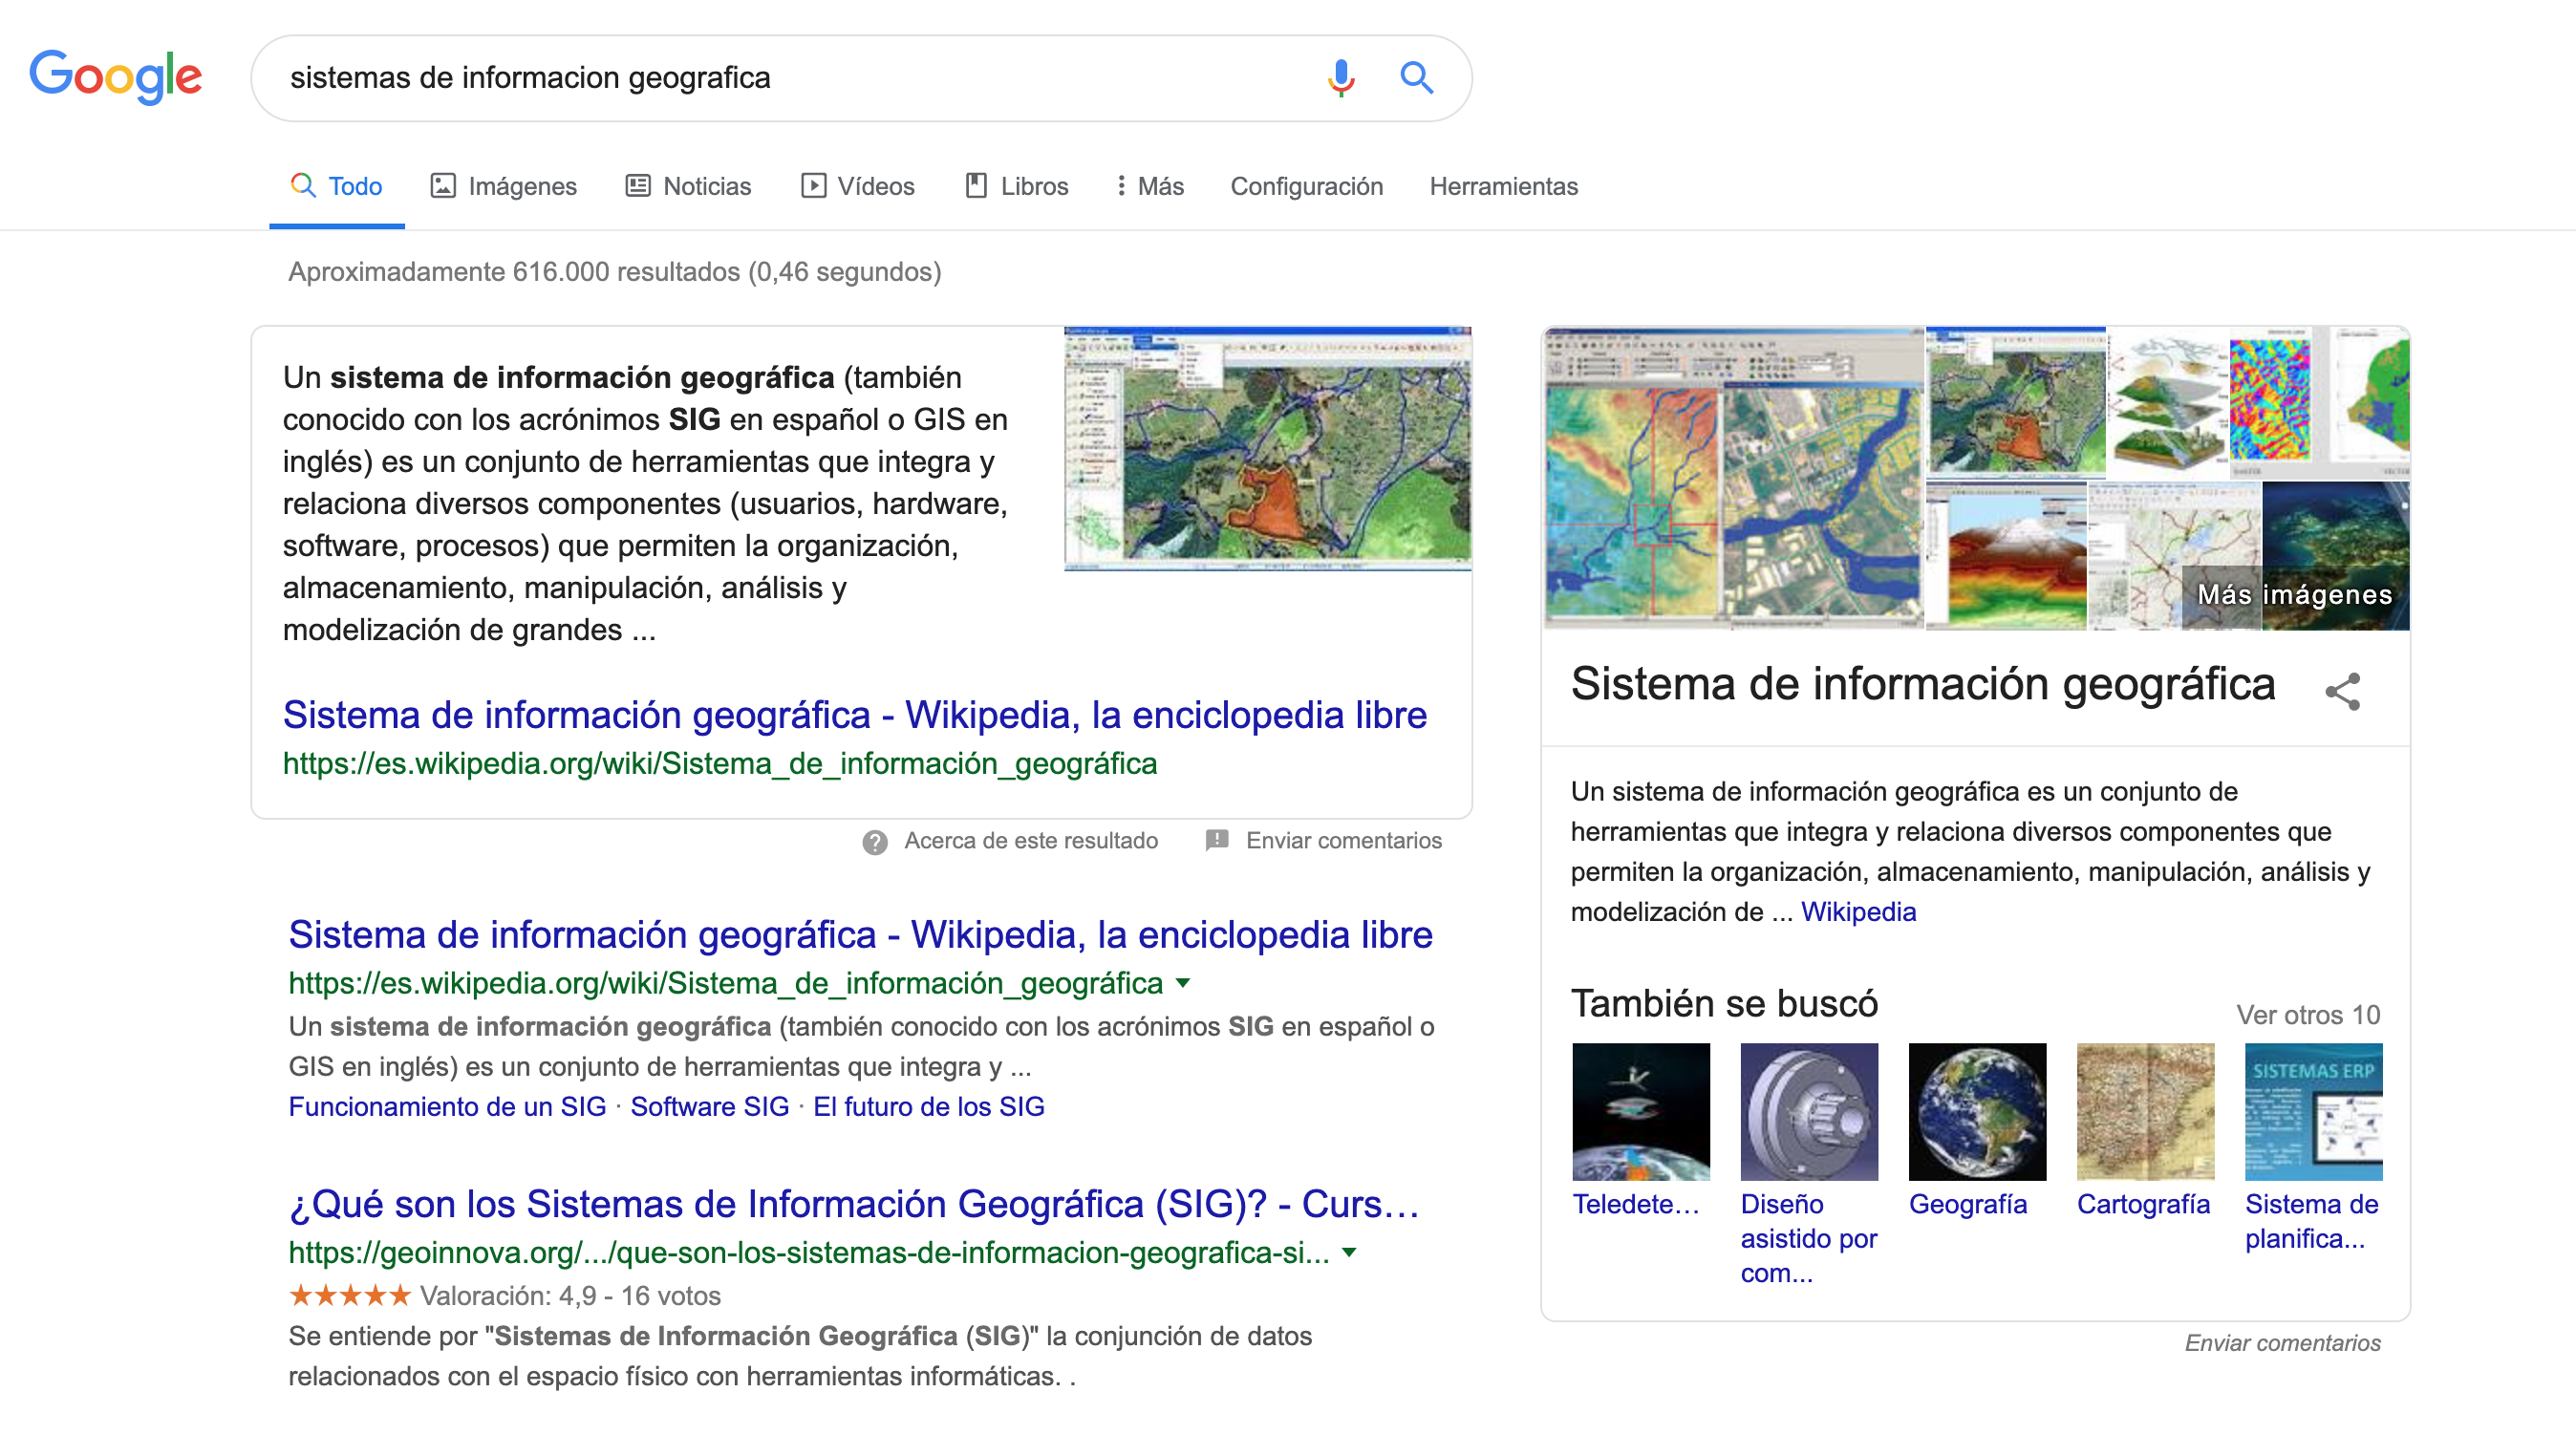
\includegraphics[width=1.07\linewidth]{imagenes/capitulo1/ejemplo-sig1}
	\caption{Ejemplo de búsqueda en Google}
	\label{fig:ejemplo-sig}
\end{figure}

En la figura \ref{fig:ejemplo-sig} se puede observar como los motores de búsquedas clásicos (Google) no interpretan la información, sino que simplemente se limitan a devolver resultados a partir de las palabras clave. En este caso se devuelven primero aquellos resultados que contienen en su título la frase ``sistemas de información geográfica''. Esto se realiza así debido a que la coincidencia de esa frase en el título del documento tiene más relevancia, que si lo encontráramos en el contenido textual de dicha página Web.\\

Por contraposición, en el mundo de los SIG, los datos geoespaciales requieren más esfuerzo técnico. Como los datos SIG son muy relevantes para muchos aspectos de la vida humana, diversos organismos tanto públicos como privados construyen fuentes geoespaciales (mapas) de alta calidad para distintas necesidades: modelos digitales del terreno, mapas de ciudades o mapas meteorológicos, entre otros; además, dictan cómo deben publicarse dichos datos de manera pública. El carácter estructurado de los datos SIG hace posible describirlos con técnicas semánticas, por ejemplo, los objetos espaciales de una capa de un mapa pueden transformarse en instancias de una clase y los atributos pueden convertirse en una propiedad de datos.\\

La capa semántica de los SIG brinda la ventaja de agregar conocimiento de dominio sobre la estructura de los datos (Edificio como una subclase de Sistema Urbano) y de vincular diversos sistemas SIG (Edificio en un SIG es una subclase de Construcción en otro). Principalmente, por la magnitud de juntar ambas tecnologías y sus posibilidades pretendo realizar una prueba de concepto que integre Información Geográfica procedente de la provincia de Granada en la Web Semántica.
% es decir, una clase de entidad en un SIG es igual o una subclase de una clase de entidad en otro SIG 


\section{Definición del problema}

% Dedique este tema a aclarar lo que pretende de hecho con su esfuerzo de investigación. El problema es la cuestión a ser respondida por el trabajo, que motivó su realización. Es una cuestión que ya se formó en su mente, derivada de teorías del área investigada y de su observación sobre un fenómeno. Normalmente se utilizan los siguientes subíndenes como medios para determinar claramente los objetivos, lo que también colabora para la delimitación del alcance del trabajo. Está estrechamente vinculado al objetivo general, que normalmente consiste en encontrar la respuesta al problema de investigación.

% ¿Qué has visto que es un problema que necesita solución? ¿Es viable? ¿Puedes hacer? El problema es siempre una dificultad, una laguna.

% Breve descripción antes de poner el objettivo de manera clara y concisa

La Web Semántica permite incorporar información muy diversa, entre ella cabe destacar la Información Geográfica. Con los conocimientos que tengo adquiridos en el área de los SIG, pretendo hacer uso de ambas tecnologías para desarrollar un ejemplo práctico que agregue conocimiento geográfico sobre la estructura de datos de la Web Semántica. \\ %De tal forma que el trabajo tiene como objetivo la integración de Información Geográfica en la Web Semántica. \\

A partir de los mecanismos para la integración de información procedente de diversas fuentes que ofrece la Web Semántica, se han definido estándares de representación de Información Geográfica mediante herramientas de la Web Semántica. En este proyecto se estudian algunas de las herramientas de la Web Semántica que se pueden utilizar para representar e integrar Información Geográfica, valorarlas y desarrollar una prueba de concepto. Se trabajará con información geoespacial, concretamente con archivos en formato \textit{Shapefile} de la provincia de Granada, en particular de mi pueblo Ogíjares y centrándonos en la información geoespacial obtenida de edificaciones, cotas de altura y curvas de nivel. En la prueba de concepto, se hará uso de las herramientas destinadas a la generación de información geoespacial (\texttt{QGIS} para permitir obtener la información de los \textit{Shapefile} a hojas de cálculo), generación de documentos \textit{RDF}  (\texttt{Protegé} para permitir llevar la información de los \textit{Shapefile} hacia documentos en formato \textit{RDF} de manera gráfica y su posterior visualización), consumo (\texttt{GraphBD} para permitir la visualización de archivos en formato \textit{RDF} y la realización de las consultas del lenguaje estándar de consulta geoespacial \textit{GEOSPARQL}) y visualización de la información geoespacial obtenida de las consultas (\texttt{R} para permitir ubicar la información geográfica en un mapa interactivo mediante la libería \textit{Shiny}).


\section{Motivación}

% Uno de los debates más habituales en la utilización de los Sistemas de Información Geográfica en entornos académicos es hasta que punto implican realmente un avance científico, con lo que su presencia como asignatura sería de pleno derecho, o si son sólo una herramienta, poco más que un procesador de textos, que los alumnos deberían aprender por su cuenta y que, como mucho, podría servir para explicar visualmente otros contenidos.

\textit{¿Qué motivación y razones me han llevado a comenzar un proyecto como este?} Cómo Ingeniera Técnica Informática y estudiante del Máster Universitario en Ingeniería Informática, he adquirido a lo largo del Grado y del Máster conocimientos y usos muy diversos que se le puede dar a la tecnología. Después de haber realizado el Trabajo de Fin de Grado en \textit{Análisis de Información Geográfica mediante QGIS y R centrado en el Modelo Digital del Terreno}, he querido seguir cumpliendo el objetivo que me propuse: conocer más el mundo en el que se mueven los SIG; puesto que en estos dos años me es imposible abarcar todas las áreas relacionadas con el mismo. Además, destacar que durante la realización del Máster Universitario en Ingeniería Informática, he adquirido algunos conocimientos en la temática de Web Semántica a partir de la asignatura de \textit{Desarrollo de Software basado en Componentes y Servicios} impartida por Manuel Ignacio Capel Tuñón. Es más, las ganas de adentrarme en este mundo, han hecho que durante este año haya asistido al curso de Web Semántica del Máster de Desarollo de Software, impartido por diversos profesores, entre ellos el tutor de este TFM. Por todo esto y más, y con la idea de pasar a un siguiente nivel mi Trabajo de Fin de Grado, surgió este Trabajo de Fin de Máster en el que intento dar cabida a la Web Semántica Geoespacial, con el fin de enriquecerme tanto personal como profesionalmente y de adentrar al lector en este tema tan interesante.\\ 

% el profesor (actual tutor) me introdujo en un ámbito que desconocía y del que apenas había oído hablar. 

% hablar sobre los cursos asistidos este año
% hablar sobre la conferencia que fui en Madrid
% hablar sobre la asignatura de SIG en el grado
% hablar sobre la asignatura de Capel

La idea de este proyecto comenzó a tomar forma a principios de curso, tras mantener varias reuniones con el tutor del TFG y ver que posibilidades había de seguir estudiando y ampliando los SIG de manera más práctica y profesional. Entonces, partiendo de todos los conocimientos que tengo a priori de la realización de este trabajo, me pregunto lo siguiente: \textit{¿existe interoperabilidad\footnote{La interoperabilidad es la capacidad de los sistemas de información y de los procedimientos a los que éstos dan soporte, de compartir datos y posibilitar el intercambio de información y conocimiento entre ellos.} en los Sistemas de Información Geográfica?} Este tipo de preguntas ha llevado a cabo el inicio del desarrollo de la prueba de concepto en donde gracias a la capa semántica que ofrecen los SIG es posible integrarlos de manera adecuada en la Web Semántica. En los sucesivos capítulos, iremos detallando cada uno de los conceptos que a lo largo de este capítulo hemos mencionamos.


% coursera
%En este curso verá en que consisten las tecnologías de la Web Semántica y como se utilizan en la web actual. También tendrá la oportunidad de realizar varios proyectos aplicando todas estas tecnologías para resolver los problemas que Marcelo ha comentado anteriormente. Por ejemplo, ¿le gustaría que Google entendiera cada uno de los componentes de su página web? O si usted tienen una tienda virtual, ¿le gustaría que Google fuera capaz de identificar los distintos productos que forman parte de su tienda virtual y los desplegara al momento de hacer una búsqueda? Esto se consigue usando [DESCONOCIDO] y les mostraremos como se relaciona en este curso con las tecnologías de la Web Semántica.

%Además, ¿le gustaría poder acceder a la Wikipedia como si fuera una tabla Excel? ¿O le gustaría poder conocer como han hecho los gobiernos para hacer públicos sus datos y de esta manera permitir que los ciudadanos puedan acceder a la información de como se gastan sus impuestos, o puedan entender de una manera más sencilla como le afecta una ley? ¿O le gustaría saber como hacen los biólogos para compartir sus datos en la web?


\section{Premisas e Hipótesis}

% La mejor forma de determinar el tema abordado es a través de premisas e hipótesis. La hipótesis consiste en una afirmación que usted considera verdadera y que va a probar o buscar probar a lo largo de su trabajo. Otra forma es delimitar el problema en forma de una pregunta de partida. Las hipótesis presentadas aquí son probadas en su trabajo es lo que llamas de tesis.

La realización de este trabajo ha partido de varios supuestos básicos: el primero parte de la posibilidad de la interoperabilidad que presentan los datos con Información Geográfica. Asumiendo, que los datos geoespaciales interoperables pueden ser utilizados por diferentes programas y aplicaciones permitiendo así el intercambio de información y conocimiento entre ellos. El segundo supuesto es un hecho y es la utilidad de integrar información estructurada de diversas fuentes en la Web Semántica, gracias a la estructura que estos presentan, para así permitir que la información contenida en las páginas Web sea entendible tanto por humanos como por máquinas. Por último, considero que este trabajo ofrece posibilidades que merecen la máxima difusión, algunas menos conocidas para gran parte del público en general y de los Ingenieros en Informática en particular.


\section{Objetivos}

% Es la respuesta al problema especificado anteriormente, es decir, lo que se pretende hacer y que, después de alcanzado, habrá terminado el trabajo. Algunos verbos utilizados para determinar el objetivo general: contribuir / facilitar / subsidiar / proponer / aclarar / permitir / agregar / comprender.

Este apartado recoge los objetivos iniciales marcados para la realización del TFM, especificando los propósitos que se esperan conseguir del mismo. A continuación, se detallan tanto los objetivos generales como específicos.

\subsection{Objetivo General}

El objetivo de este proyecto es profundizar \textbf{en las herramientas de la Web Semántica que se pueden utilizar para representar e integrar Información Geográfica, valorarlas y desarrollar una prueba de concepto}. Para ello, se hará uso de las distintas posibilidades que existen actualmente para la Web Semántica Geospacial. Así que, mediante este proyecto se adquirirá experiencia en la Web Semántica y en el uso de sus herramientas para combinar información procedente de los SIG.

\subsection{Objetivos Específicos}

% Los objetivos específicos detallan los objetivos generales a través de etapas o fases de investigación. Se deben utilizar verbos en el infinitivo, señalando las acciones propuestas para alcanzar el objetivo general. Los verbos utilizados aquí son los de acción, que serán utilizados en la metodología.

% Comprobar si los objetivos puestos del principio corresponden con los objetivos que he cumplido al terminar el trabajo

En el subapartado anterior, se mencionan a grandes rasgos los objetivos que vamos a lograr con dicho estudio y aplicación. Por tanto, detallaremos los objetivos más específicos del proyecto, en donde al final del documento comprobaremos que se han cumplido:

\begin{enumerate}
	
	\item \textbf{Conocer diversas fuentes de información}, con las que obtener datos públicos geográficos de buena calidad.
	
	\item \textbf{Comprender la relación existente entre los Sistemas de Información Geográfica y la Web Semántica}, a priori dos áreas completamente diferentes.
	
	\item \textbf{Localizar diversas herramientas de la Web Semántica} que se puedan utilizar para representar e integrar Información Geográfica.
	
	\item \textbf{Aprender a crear ontologías y poblarlas} mediante información geográfica existente.
		
	\item Aprender a \textbf{agregar conocimiento de dominio geoespacial sobre la estructura de los datos} mediante el empleo de herramientas de la Web Semántica como Protegé.
	
	\item Apreciar las carencias o mejoras que supone usar \textbf{Protegé frente a otro tipo de herramientas}.
	
	\item Conocer cuál es la \textbf{estructura de los datos geoespaciales para realizar consultas con GeoSPARQL}.
	
	\item Mostrar algunos \textbf{métodos de trabajo}, estrechamente adaptados al tratamiento de Información Geográfica en la Web Semántica.
	
	\item \textbf{Aportaciones a la comunidad o al lector}, para que el proyecto sirva como puerta de acceso al mundo de la Web Semántica y en particular, al de la Web Semántica Geoespacial, y facilite el acceso a parte de los conocimientos actuales disponibles.
	
	\item \textbf{Aportaciones hacia mi persona} en la adquisición de conocimientos de la Web Semántica, creación de ontologías, manejo de herramientas semánticas como Protegé y aprendizaje para la creación de un mapa interactivo mediante la librería Shiny de R.	

	
	%\item \textbf{Análisis exhaustivo de los MDT}, contemplando las posibilidades que presentan para su futura aplicación en el ámbito de los SIG.
	
	%\item Aprender a \textbf{manipular información del terreno} mediante el empleo de herramientas como QGIS y R.
	
	%\item Apreciar las carencias o mejoras que supone el \textbf{uso de R frente a QGIS}.
	
	%\item Analizar un MDT con diversos paquetes de R y en consecuencia, \textbf{crear un paquete en R} que encapsule el análisis de sombras.
	
	%\item \textbf{Conocer diversas fuentes de información}, con las que obtener datos precisos del terreno y de buena calidad.
	
	%\item Mostrar algunos \textbf{nuevos métodos de trabajo}, estrechamente adaptados al tratamiento digital de la información y actualmente en rápido desarrollo. % Para ello, se expondrán las bases conceptuales, así como métodos de construcción y tratamiento de los modelos digitales del terreno (MDT), un caso de enorme interés dentro del conjunto de la cartografía digital.
	
	%\item \textbf{Aportaciones a la comunidad o al lector}, para que el proyecto sirva como puerta de acceso al mundo de los SIG y facilite el acceso a parte de los conocimientos actuales disponibles.
	
	%\item \textbf{Aportaciones hacia mi persona} en la adquisición de conocimientos SIG, manejo de herramientas como QGIS y R, análisis de MDT para mapas de sombras y aprendizaje para la creación de una librería en R.

\end{enumerate}


\section{Estructura de la monografía}

% En este ítem usted describirá cómo está constituida la monografía, indicando lo que será encontrado en cada una de las sesiones siguientes.

En este primer capítulo, se ha desarrollado una pequeña introducción al contexto que desarrolla este trabajo, puntualizando en los motivos de la elección del mismo. A continuación, se detallan de forma resumida los contenidos del resto de capítulos de este documento:

\begin{itemize}
	\item En el \textit{capítulo 2} \textbf{(Sistemas de Información Geográfica)}, se presentan los SIG, en donde, veremos brevemente el estado del arte sobre ciertos aspectos relacionados con el proyecto, necesarios para entender las especificaciones de los datos geográficos que vamos a usar.
	
	\item En el \textit{capítulo 3} \textbf{(Web Semántica)}, se expone el concepto de Web Semántica, y las capas o tecnologías que conforman su arquitectura, necesarios para comprender su uso y aplicación en las herramientas y tecnologías usadas en el \texttt{capítulo 4}.
	
	\item En el \textit{capítulo 4} \textbf{(Prueba de Concepto)}, se abarca el trabajo realizado por mí, en donde se realiza la prueba de concepto para integrar Información Geográfica procedente de la Junta de Andalucía, en concreto de la provincia de Granada, en la Web Semántica, gracias a las herramientas disponibles, las cuales se estudian y valoran para permitir desarrollar dicha prueba de concepto de manera adecuada y de acuerdo con los estándares establecidos.
	
	%El trabajo que se presenta a continuación es un estudio sobre la necesidad de \textbf{integrar Información Geográfica en la Web Semántica mediante el uso herramientas específicas}. A partir de la Información Geográfica disponible en la Junta de Andalucía y centrándonos en la información geoespacial de edificaciones, curvas de nivel y cotas de altura de Ogíjares (Granada), es posible realizar una prueba de concepto gracias a la integración que los SIG presentan en la Web Semántica.\\
	
	%\item En el \textit{capítulo 5} \textbf{(Resultados)}, 

	\item En el \textit{capítulo 5} \textbf{(Conclusiones y Trabajo Futuro)}, se evalúan las propuestas realizadas en el \texttt{capítulo 4}, recopilando tanto lo que se ha hecho a lo largo del desarrollo de este trabajo como las conclusiones y resultados finales obtenidos de esta experiencia. Se comentan además una serie de mejoras para el futuro que se podrían aplicar, pero que por diversos motivos caen fuera del ámbito de este trabajo.
	
	\item En el \textit{Anexo A} (planificación del trabajo)
	
	\item En el \textit{Anexo B} (evolución de la Web)
	
	\item En el \textit{Anexo C} (¿Linked Data?)
		
	\item En el \textit{Anexo D} (errores y soluciones obtenidos)
			
	%\item Por último se incluye un \textbf{(Apéndice)}, que incorpora material adicional que complementa la información de algunos de los capítulos de este documento.
	
\end{itemize}


%\begin{figure}[H]
%	\centering
%	\includegraphics[height=4.5cm]{imagenes/4_solsticio-equinoccio.jpg}
%	\caption{Solsticios y Equinoccios para las 12 a.m.}
%	\label{fig:solsticio-equinoccio}
%\end{figure}
% Conceptos Generales y Revisión de la Literatura

% En este capítulo debe ser proporcionado el estado del arte o referencial teórico sobre el tema al que se refiere el estudio. Un buen investigador no debe repetir trabajos ya concluidos o que ya están en marcha. Por eso esta sesión es donde el autor demuestra hasta dónde va la investigación actual en el campo de estudios en cuestión y establece las bases sobre las cuales desarrollará el estudio propuesto. También este punto se podría denominar "Situación actual de la tecnología". No se habla del estado actual de la tecnología con la que se desarrollará el trabajo, sino de qué otras aplicaciones que existen actualmente o han existido en el mercado (historia de la evolución tecnológica) y que realicen funcionalidades iguales o parecidas a las que se propone desarrollar en el TFG. En este punto hay que presentar lo que hay, simplemente describiendo. Se puede hacer alguna pequeña valoración que muestre los puntos fuertes de la tecnología o su utilidad, en que ámbitos se puede aplicar, para posteriormente, en el apartado de "Crítica al estado del arte" enjuiciar constructivamente cada aportación y de ahí extraer consecuencias para el TFG.

\chapter{Conceptos Geográficos}
\label{ch:sig}

\begin{quote}
  {\bf\textsc{Resumen:}} Este capítulo ...
\end{quote}

% coger lo del TFG y modificarlo y adaptarlo un poco, y ver algún enlace nuevo  

\section{Sistemas de Información Geográfica}



% Definición de los SIG

% https://www.ceupe.com/blog/los-sistemas-de-informacion-geografica.html


\subsection{Elementos de un SIG}


\subsection{Ejemplo de aplicación real de los SIG}



\section{?`Qué no es un SIG?}




\section{Tipos de SIG}


\subsection{Representación de datos geográficos}

- Modelo de datos Ráster
- Modelo de datos Vectorial

\subsection{Tipos de software SIG}


Hay varios SIG comerciales de escritorio: ESRI ArcGIS, Intergraph GeoMedia, Autodesk Au-toCAD, MapInfo Professional, Smallworld GIS y SuperMap.\\

Además, numerosos sistemas de software GIS de escritorio de fuente abierta también están disponibles para el manejo de datos geoespaciales: GRASS GIS, gvGIS, JUMP GIS, uDig, SAGA GIS, ILWIS, MapWindow GIS y QGIS.\\

Es improbable que todas las aplicaciones GIS utilicen el mismo software. Los diferentes proveedores tienen sus propios diseños de software propietario, modelos de datos y estructuras de almacenamiento de bases de datos. Por lo tanto, las bases de datos geográficas basadas en estos diseños no pueden comunicarse sin la conversión de datos. Para intercambiar información y compartir recursos de geo-bases de datos computacionales entre sistemas heterogéneos, se deben desarrollar herramientas de conversión para transferir datos de un formato a otro. Además, estas diversas estructuras de bases de datos SIG de escritorio hacen que el intercambio de datos remoto y el intercambio sean más difíciles debido a la accesibilidad limitada y la conversión de datos requerida.\\

Internet GIS o Web GIS crea un entorno único para compartir datos geoespaciales. Hay muchos programas de Internet GIS o Web GIS disponibles para compartir datos a través de la Web, como Esri’s ArcGIS Server, Intergraph’s GeoMedia WebMap, MapInfo’s MapExtreme, AutoDesk’s MapGuide, GE SmallWorld’s Internet Application Server y ER Mapper’s Image Web Server.\\

Aunque estos programas de Internet GIS ofrecen mejores herramientas para compartir datos en la Web, también tienen los problemas de los diseños de software propietario, los modelos de datos y las estructuras de almacenamiento de bases de datos. El intercambio de datos, facilitado por los avances en las tecnologías de red, se ve obstaculizado por la incompatibilidad de la variedad de modelos y formatos de datos utilizados en diferentes sitios.


\section{Resumen del capítulo}


% Aquí contendrán los métodos y procedimientos adoptados en el desarrollo del trabajo. Esta es una de las sesiones más importantes pues demuestra el poder científico que se utilizó para la investigación. Sin una buena metodología la investigación puede perder la validez. El investigador debe utilizar métodos o técnicas aceptadas por la comunidad científica en la búsqueda de probar sus hipótesis.

% La metodología elegida debe ser aquella que más se adecue a su objeto de estudio y al enfoque aplicado. Hay dos métodos principales: 1) cuantitativo, que es el uso de instrumental estadístico, de datos numéricos; y 2) cualitativo, que se caracteriza por la calificación de los datos recogidos, durante el análisis del problema.

% ENLACES VISTOS
% COURSERA: La Web Semántica: Herramientas para la publicación y extracción efectiva de información en la Web
% CURSO EN COURSERA INTERESANTE: https://es.coursera.org/learn/web-semantica?action=enroll
% http://www.fgcsic.es/lychnos/es_es/articulos/construyendo_una_web_semantica
% Libro Geospatial Semantic Web
% https://www.researchgate.net/publication/216537707_La_Web_semantica_y_las_tecnologias_del_lenguaje_humano
% http://www.bibliopos.es/Biblion-A2-Bibliografia-Documentacion/18ontologia-Web-Semantica.pdf

\chapter{Web Semántica}
\label{ch:web-semantinca}

\begin{quote}
  {\bf\textsc{Resumen:}} En este capítulo se presenta la Web Semántica como una extensión de la Web actual que nos ayuda a encontrar respuestas a preguntas en Internet haciendo uso de la información semántica contenida en la búsqueda. Los conocimientos que adquiramos a lo largo de este capítulo sirven como base para el posterior desarrollo del ejemplo práctico. De esta manera, dividiremos el capítulo en tres grandes apartados: el primero contextualiza y explica la Web Semántica, el segundo nos adentra en las capas de la arquitectura de la Web Semántica, y el tercero habla sobre aplicaciones que presenta la Web Semántica.
\end{quote}

\section{Web Semántica}

A continuación, vamos a introducir la definición de Web Semántica, para ello es necesario realizar un breve estudio del arte sobre la Web actual, para así comprender su origen y contexto en el que nace.

\subsection{Conceptos generales}

%% ANTECEDENTES
%% DEFINICIÓN DE WEB, CUANDO SE CREO, QUIEN LA CREO, COMO SURGIÓ

% https://disenowebakus.net/semantica-web.php
% tesis
La revolución informática, acaecida durante el siglo XX, llevó consigo la introducción de cambios severos en distintos aspectos de la sociedad. De entre todas estas transformaciones, fueron muchos los que vaticinaron un nuevo mundo, fundamentado principalmente por la aparición de la informática personal, en donde los seres humanos tendrían acceso a grandes repositorios de información \cite{semantica-web}. Este hecho trajo consigo el desarrollo, por parte del físico Tim Berners-Lee del CERN\footnote{El \href{https://home.cern}{CERN}, Organización Europea para la Investigación Nuclear, es uno de los centros de investigación científica más grandes y respetados del mundo ubicado en Suiza.}, de un sistema de vinculación y transferencia de documentos en red que acabaría convirtiéndose en la World Wide Web (WWW) o Red Global Mundial, actualmente conocida como la \textbf{Web} \cite{tesis}.
%.creada por Tim Berners-Lee en 1989 y presentada en el CERN\footnote{El \href{https://home.cern}{CERN}, Organización Europea para la Investigación Nuclear, es uno de los centros de investigación científica más grandes y respetados del mundo.} (Suiza) \cite{tesis}. \\

% https://www.researchgate.net/publication/216537707_La_Web_semantica_y_las_tecnologias_del_lenguaje_humano
% COURSERA: La Web Semántica: Herramientas para la publicación y extracción efectiva de información en la Web
A lo largo de la literatura, muchos son los autores que han definido la Web Semántica como la Web del futuro. Sin embargo, para poder comprenderla es necesario entender bien cuál es la Web actual \cite{researchgate}. En términos generales, la Web actual es una red informática compuesta por multitud de documentos \cite{coursera}. Estos documentos son básicamente páginas Web que hacen uso del lenguaje natural para expresar sus contenidos (texto, imágenes, audios, enlaces) y de etiquetas HTML (\textit{HyperText Markup Language}) para su interpretación en los navegadores Web (Figura \ref{html}). 

% https://fjph32html.wordpress.com/2015/03/08/leccion-3-estructura-basica-en-html/
\begin{figure}[H]
	\centering
	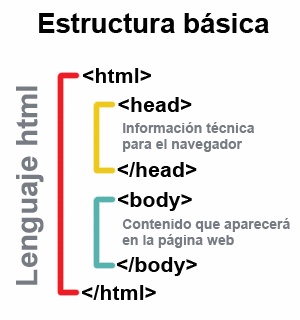
\includegraphics[height=5.1cm]{imagenes/capitulo3/estructurabasica} 
	\caption{Ejemplo de la estructura HTML \cite{imagen-html}}
	\label{html}
\end{figure}

Una de las principales causas del éxito de la Web se debe a la implantación como formato universal del lenguaje HTML (Figura \ref{html}). Gracias a este lenguaje, los ordenadores pueden analizar la estructura de las páginas Web, determinar cuál es la cabecera o indicar dónde hay un enlace a otra página. Sin embargo, no tienen una manera fiable de procesar la semántica de las páginas, lo que convierte a la Web actual en una Web Sintáctica cargada de documentos HTML diseñados sólo para ser leídos por humanos \cite{apuntes-clase-jose}.\\

Adicionalmente, la Web surgió con navegadores básicos que sólo interpretaban texto, después apareció HTML haciendo las páginas más amigables y de fácil acceso. En la figura \ref{evolucion:web} podemos ver que la Web ha pasado por distintas fases desde su primera generación, en donde las personas con conocimiento específico de diseño y composición de páginas Web crean documentos con contenido y definen los hipervínculos que los entrelazan para que los usuarios no expertos consuman esta información \cite{cwb}; pasando por la  Web 2.0 que busca que los usuarios interactúen con las páginas Web que visitan y se sientan como parte de la experiencia; hasta la evolución de la Web 2.0 conocida como Web 3.0, y en ocasiones confundida con la Web Semántica, es decir, la Web 3.0 es lo que se experimenta a diario en el dispositivo móvil al abrir la aplicación de Twitter, que te permite consultar la información de la red social sin necesidad de abrir el navegador \cite{web-nueva}.

\begin{figure}[H]
	\centering
	\begin{subfigure}[h]{0.22\textwidth} 
		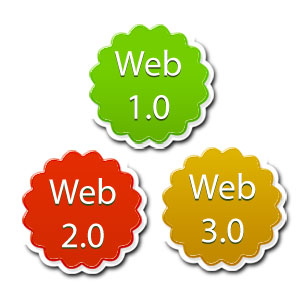
\includegraphics[width=\textwidth]{imagenes/capitulo3/what_s-the-difference-between-web-1-0-web-2-0-web-3-0}
		\caption{}
	\end{subfigure}       
	\begin{subfigure}[h]{0.49\textwidth} 
		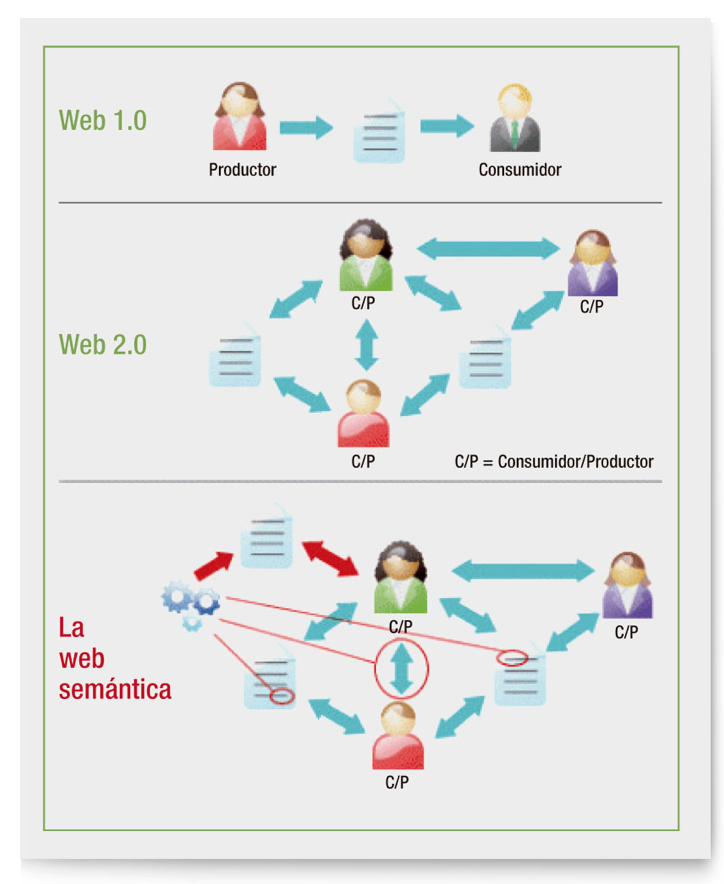
\includegraphics[width=\textwidth]{imagenes/capitulo3/10}
		\caption{}
	\end{subfigure}
	\caption{Evolución de la Web \cite{web-tipos, cwb}}
	\label{evolucion:web}
\end{figure}


%\begin{figure}[H]
%	\centering
%	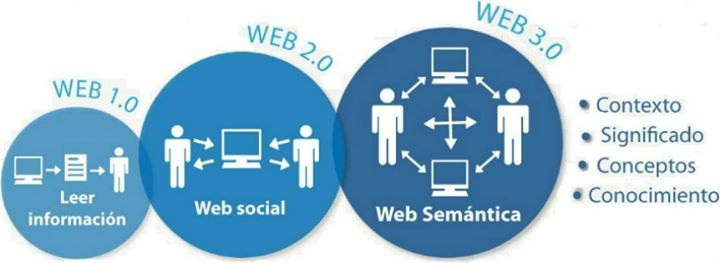
\includegraphics[width=0.67\linewidth]{imagenes/capitulo3/WEB}
%	\caption{Evolución de la Web Semántica}
%	\label{fig:web}
%\end{figure}



% FUNCIONALIDAD WEB ACTUAL

% Apuntes clase Jose
% COURSERA: La Web Semántica: Herramientas para la publicación y extracción efectiva de información en la Web



La Web Sintáctica, la que usamos actualmente, hace alusión a la búsqueda de información sin interpretación del significado. Por ejemplo, si se escribe en Google la frase ``\textit{la buena lectura}'', el navegador buscará en que páginas aparecen esas tres palabras, es decir, dicha búsqueda se hace sin tener en cuenta el significado que pueda tener la frase. Por ejemplo, en la figura \ref{ejemplo} podemos apreciar como dicha búsqueda nos devuelve páginas en cuyo título aparecen al menos dos de las tres palabras de nuestra frase. Esto se debe a que el enfoque clásico de buscar en la Web se basa en similitudes y sinónimos generales de texto y palabras, además de en el uso de estadísticas, lo que dificulta limitar los resultados que un usuario desea. De esta manera, el usuario debe seguir un proceso iterativo para encontrar las palabras clave adecuadas para la obtención de los resultados esperados.\\



Otro ejemplo para la Web podría ser el mostrado en la figura \ref{fig:wikipedia}, en donde podemos ver una página Web (Wikipedia) con la descripción de la WWW \cite{coursera}. La mayoría de nosotros estamos familiarizados con Wikipedia, y cuando accedemos a ella no nos supone mucha dificultad distinguir su contenido textual, sus imágenes o sus enlaces en color azul para redirigirnos a otras páginas Web con otros contenidos totalmente distintos. Entonces \textit{¿cómo podría una aplicación consumir datos de dos Webs distintas?} o \textit{¿cómo sabría qué contenido leer dentro de cada página Web?} Ambas preguntas podrán ser contestadas una vez finalizado el presente trabajo.

\begin{figure}[H]
	\centering
	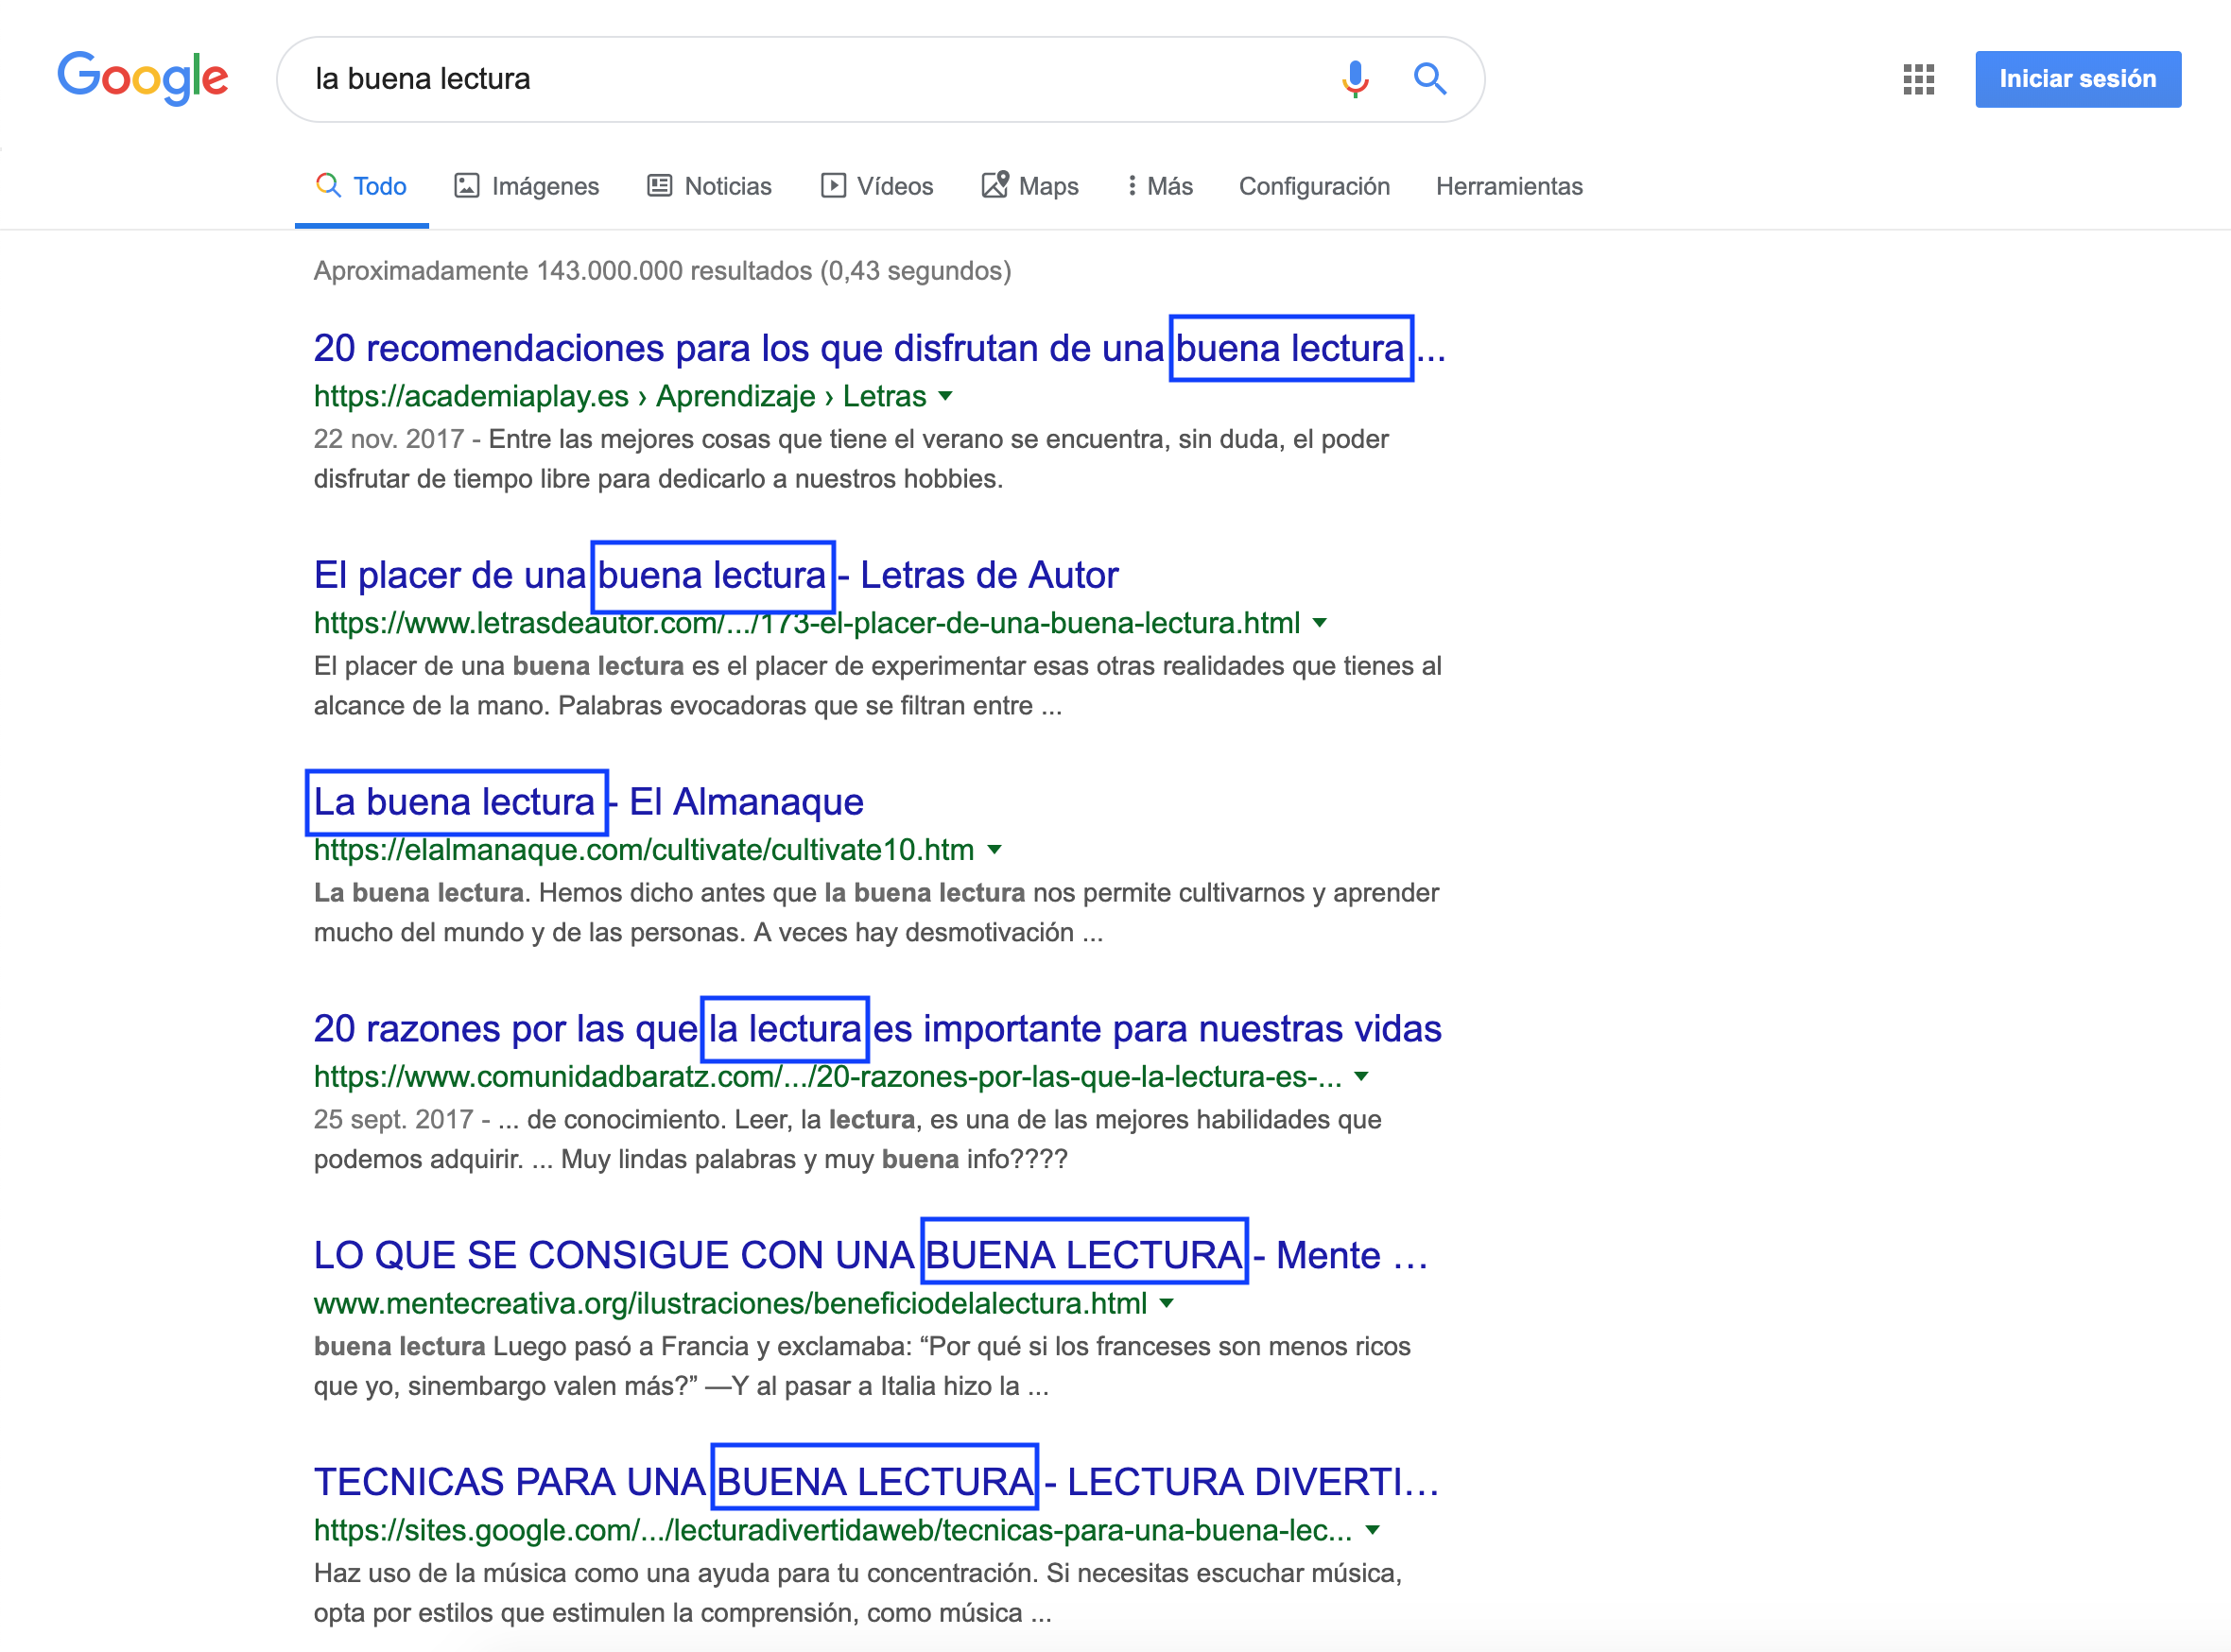
\includegraphics[height=9.5cm]{imagenes/capitulo3/ejemplo}
	\caption{Ejemplo de la búsqueda ``\textit{la buena lectura}'' en Google}
	\label{ejemplo}
\end{figure}

\begin{figure}[H]
	\centering
	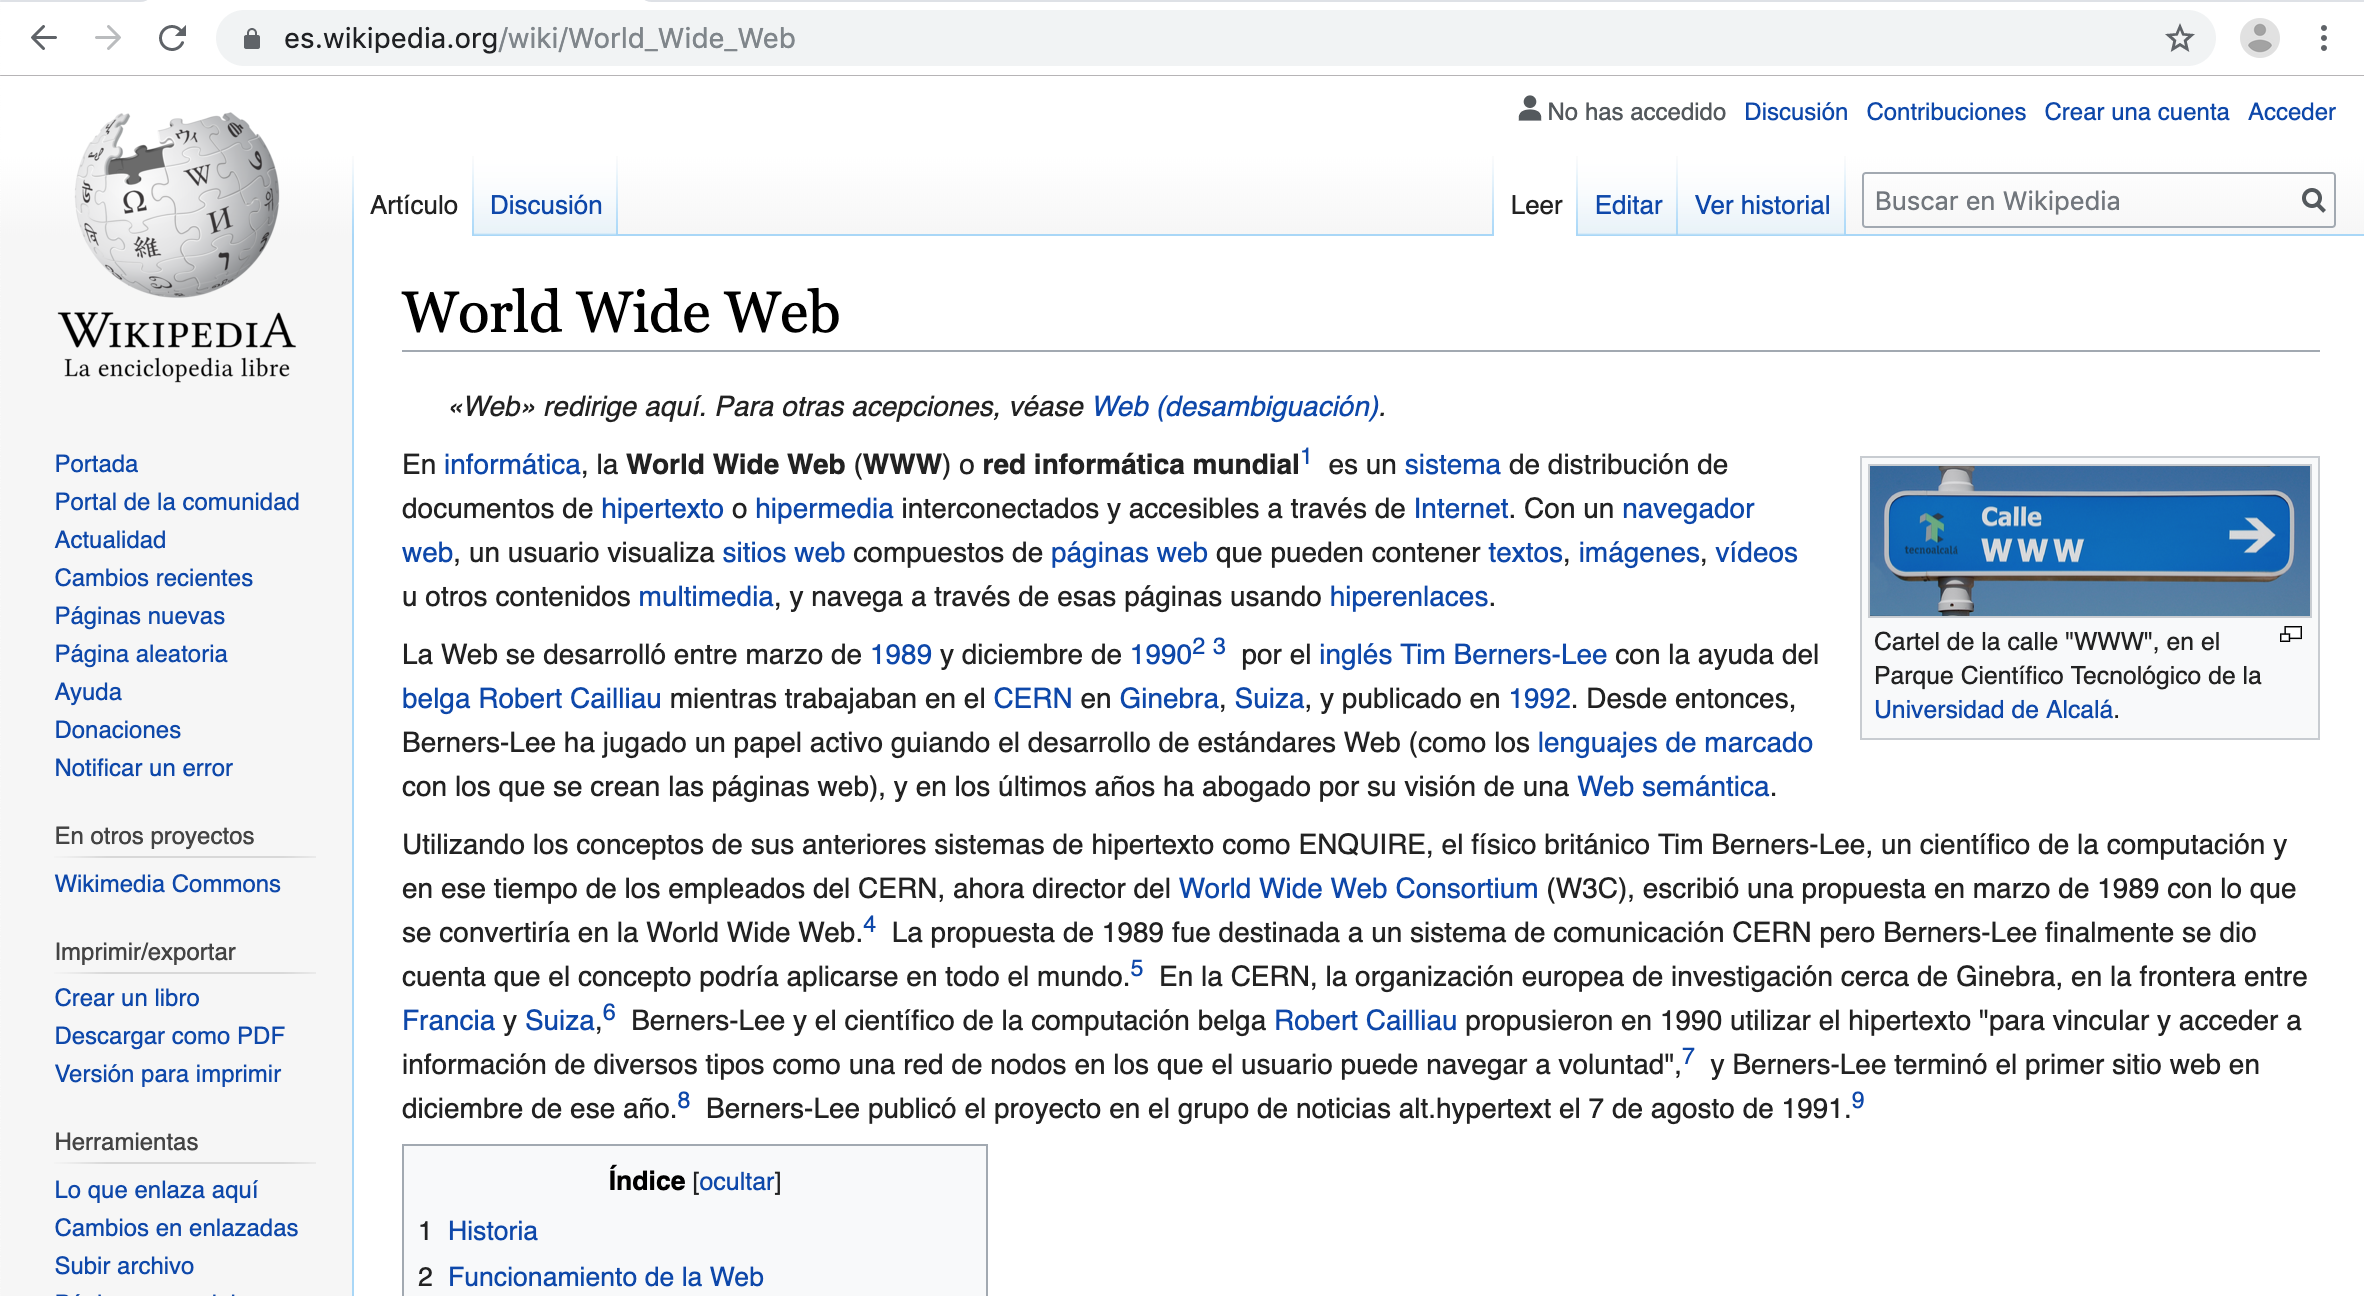
\includegraphics[height=6.95cm]{imagenes/capitulo3/wikipedia}
	\caption{Entrada en Wikipedia para la WWW}
	\label{fig:wikipedia}
\end{figure}


% EJEMPLO 1 DE WEB ACTUAL


% Leyendo el texto, el contenido. Pero, ¿cómo sabe qué contenido leer dentro de una página web? Mirando el código HTML de cada página. Podría ser pero es muy desordenado. Por dentro el código está muy desordenado siempre. Uno no sabe, una aplicación no sabría exactamente dónde está el nombre de una persona dentro del código html. Normalmente es muy difícil de saber.

% http://www.fgcsic.es/lychnos/es_es/articulos/construyendo_una_web_semantica
%Todos estamos bastante familiarizados con la Web y cómo operar con ella. Abrimos un navegador (por ejemplo, Chrome, Explorer, Firefox o Safari) e introducimos la dirección de la página que deseamos consultar o bien pedimos a un buscador (por ejemplo Google, Bing o Yahoo!) que nos determine las ubicaciones de documentos en la Web que contengan una combinación de palabras deseada y que nos las ordene por importancia.­


% http://www.bibliopos.es/Biblion-A2-Bibliografia-Documentacion/18ontologia-Web-Semantica.pdf
% https://www.w3c.es/Eventos/2009/Talleres/Murcia/Presentaciones/jesualdo.pdf

% [ejemplo arquitectura de como funciona la web actual]
% [mencionar algo de pubmed]

% ENTIENDO QUE ES LA WEB ACTUAL
% DESAFÍOS QUE PRESENTA LA WEB ACTUAL

% COURSERA: La Web Semántica: Herramientas para la publicación y extracción efectiva de información en la Web
Seguidamente, una vez entendida la Web actual, es necesario comprender los desafíos que presenta (tabla \ref{desafios}). Para ello debemos empezar diciendo que la Web actual es masiva (\textit{¿cuántos millones de páginas Web existen en la red?}), cambiante (\textit{¿cuántos tweets se generan en un segundo?}), heterogénea (\textit{¿cuántos millones de dispositivos independientes generan datos en un día?}) y está hecha para humanos \cite{coursera}.

\begin{table}[H]
	\centering
	\caption{Desafíos que presenta la Web actual \cite{coursera}}
	\label{desafios}
	\begin{tabular}{|>{\columncolor[HTML]{EFEFEF}}l |m{7.75cm}|}
		\hline
		\textbf{Heterogénea} & Múltiples organizaciones generan datos de forma independiente \\ \hline
		\textbf{Masiva} & La cantidad de información existente es enorme \\ \hline
		\textbf{Cambia muy rápido} &  Cada día son publicados y borrados enormes
		vólumenes de información\\ \hline
		\textbf{Hecha para humanos} &  En general, una persona puede interpretar la información de una página Web\\ \hline
	\end{tabular}
\end{table}



%\begin{figure}[H]
%	\centering
%	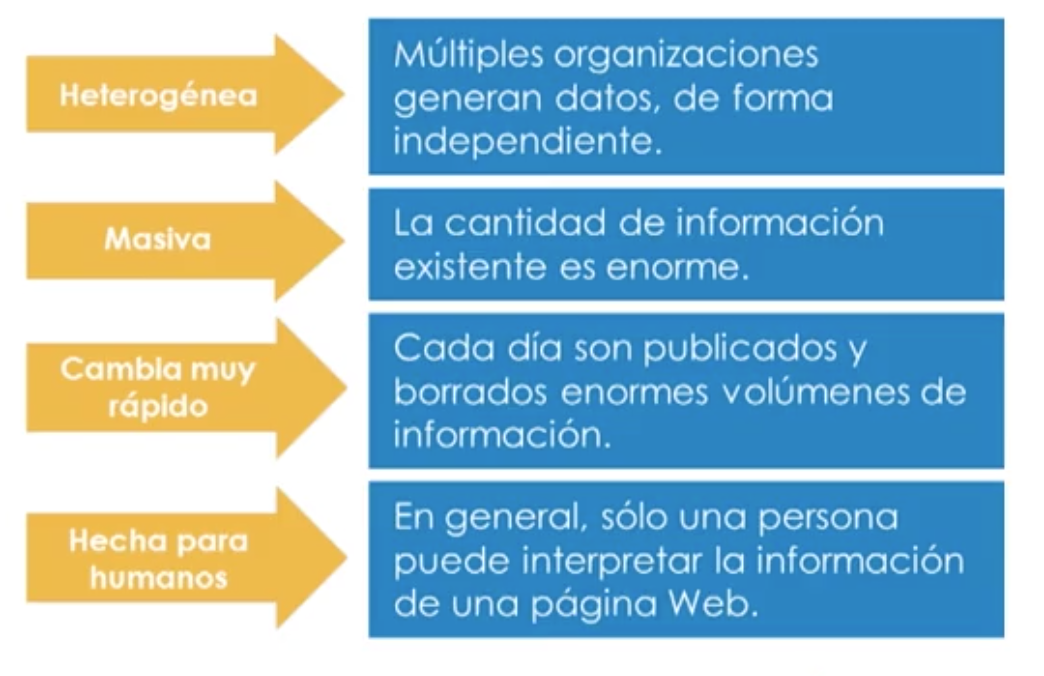
\includegraphics[height=6cm]{imagenes/capitulo3/1} % Características de la WEB
%	\caption{}
%	\label{desafios}
%\end{figure}



%\begin{enumerate}

% Heterogenea
% El primer desafío es la heterogeneidad. Como hemos visto, la Wikipedia tiene un formato, PubMed tiene otro formato, Facebook tiene otro formato de datos, nos presenta las cosas de forma distinta. Es decir la web es muy heterogénea.
%\item \textbf{Heterogénea}: ¿Cuántos millones de dispositivos independientes generan datos en un día? En la red existen muchas páginas web que son capaces de generar mucha cantidad de datos, y presentarlos de manera totalmente distinta a los usuarios. Por ejemplo, las redes sociales como 
%Tanto las páginas web como aplicaciones web generan muchos datos, los cuales y los presenta de manera totalmente distinta a los usuarios. No es lo mismo lo que se hace en todas las redes sociales, como por ejemplo Twitter o Facebook, ya que son totalmente distintas y no intercambian datos entre ellas.

% Masiva
% ¿Y cómo es la web actual? Primero la web actual es masiva. 
% Además la web es masiva. Hay muchísimos datos en PubMed, en Wikipedia, en Facebook. Hay una cantidad ingente de datos. Además cambia muy rápido. Por ejemplo, yo podría estar actualizando mi perfil de Facebook cada hora, cada dos horas. Hay gente que lo actualiza cada 15 minutos. Entonces todo esto cambia muy rápido y estoy dando un ejemplo muy chiquito, muy concreto. Además la web es masiva. Por ejemplo, la Wikipedia son casi 6 terabytes de datos. Y ¿qué es un terabyte de datos? En un terabyte de datos caben 678 millones de páginas de texto. 678 millones, eso, suponiendo que el Quijote tiene 1.000 páginas de texto, quiere decir que en un terabyte caben 678 mil Quijotes, Y en una Wikipedia, con 6 terabytes de datos, caben alrededor de 4 millones de Quijotes. Muchísimo.

%\item \textbf{Masiva}: ¿Cuántos millones de páginas web existen? Hoy en día, páginas como Wikipedia o Twitter generan muchísimos datos cambiantes. Por ejemplo, es posible estar actualizando mi perfil cada hora. 

% Cambia muy rápido
%  Además la web actual es cambiante  ¿Cuántas actualizaciones de perfil de Facebook se generan? Incontables,
% Esos son 27 Wikipedias por segundo. Se transfieren alrededor de Internet 27 Wikipedias cada segundo. Eso es muchísimo.
%\item \textbf{Cambia muy rápido}: ¿Cuántos tweets por segundo se generan? Actualmente se transfieren en Internet 160 terabytes de datos por segundo, lo que genera que cambie muy rápido. 

% Hecha para humanos
% La web actual además es distribuida, cualquier persona en el mundo puede acceder o generar contenido, no solo esto la web actual es un gran repositorio de información al cual todo el mundo puede acceder.
% Además la web está hecha para humanos. Como comentaba anteriormente Facebook lo consumen principalmente las personas. La Wikipedia la consumen normalmente las personas. Pero ¿qué pasa si yo quiero enlazar o combinar los datos de la Wikipedia y de Facebook o la Wikipedia y de PubMed? Eso actualmente, con el diseño de la web actual no es posible.
%\item \textbf{Hecha para humanos}: Si nos hemos fijado hasta el momento, los ejemplos que he puesto, la Wikipedia, Twitter o Facebook, están hechas para que sean consumidos por las personas. Las máquinas, el software no tiene tanto acceso a este contenido. Es difícil para un programa interpretar los datos que hay, por ejemplo, en el perfil de Facebook de una persona. o dentro de la Wikipedia. 

%\end{enumerate}

% ENTENDER LA WEB ACTUAL (RESUMEN DEL PARRAFO)
% INTRODUCIR AL FINAL LA WEB SEMÁNTICA (VER COMO HACERLO) Y ASÍ UNIRLO AL SIGUIENTE APARTADO

% https://disenowebakus.net/semantica-web.php
% COURSERA: La Web Semántica: Herramientas para la publicación y extracción efectiva de información en la Web
% LA ONTOLOGÍA Y LA WEB SEMÁNTICA: RECOMENDACIONES DEL W3C. 
% RAE
% Apuntes clase Jose

En consecuencia, podemos concluir que la Web se ha impuesto como el instrumento de uso cotidiano más potente y rápido para el intercambio y/o difusión de información en nuestra sociedad, accesible toda ella a través de Internet. No obstante, su capacidad para satisfacer necesidades específicas es limitada. Entonces, \textit{¿es realmente accesible esta información?} Hoy en día, existen numerosas herramientas como Google, Yahoo! o Bing que nos facilitan el acceso a esos datos \cite{semantica-web}. Sin embargo, estas herramientas tienen dificultades a la hora de entender la información que está contenida en ellas. Asimismo, la abrumadora obtención de resultados, tanto relevantes como irrelevantes a partir de una búsqueda, denota una importante falta de precisión en la Web \cite{coursera}. Este inconveniente se debe principalmente a que la Web actual carece de capacidad para expresar significados. En particular, estas herramientas miran las páginas Web como si fueran un conjunto de palabras, limitándose a recoger cadenas de caracteres indexadas en grandes bases de datos o a buscar palabras clave, y presentarlas en la pantalla del ordenador para su posterior visualización (Figura \ref{ejemplo}) \cite{web-semantica-w3c}. Por lo cual, estas herramientas no son capaces de entender los elementos que forman parte de ella (lugares geográficos, actores, películas) y las relaciones existentes entre estos elementos, lo que dificulta que el ordenador no sepa realmente lo que significa la información, puesto que la mayoría de los contenidos de la Web actual están diseñados para ser leídos por humanos \cite{apuntes-clase-jose}. \\

% tesis
%En la actualidad, la Web esta compuesta por varios documentos distribuidos en diferentes lugares del planeta, durante muchos años ha sido una poderosa herramienta para publicar, buscar y compartir información  convirtiéndose en una gran base de datos, siendo imposible explotar adecuadamente esa información. 
%\begin{figure}[H]
%	\centering
%	\includegraphics[height=5.6cm]{imageness/capitulo3/bing} 
%	\caption{Página inicial del buscador Bing}
%	\label{bing}
%\end{figure}

%\begin{figure}[H]
%	\centering
%	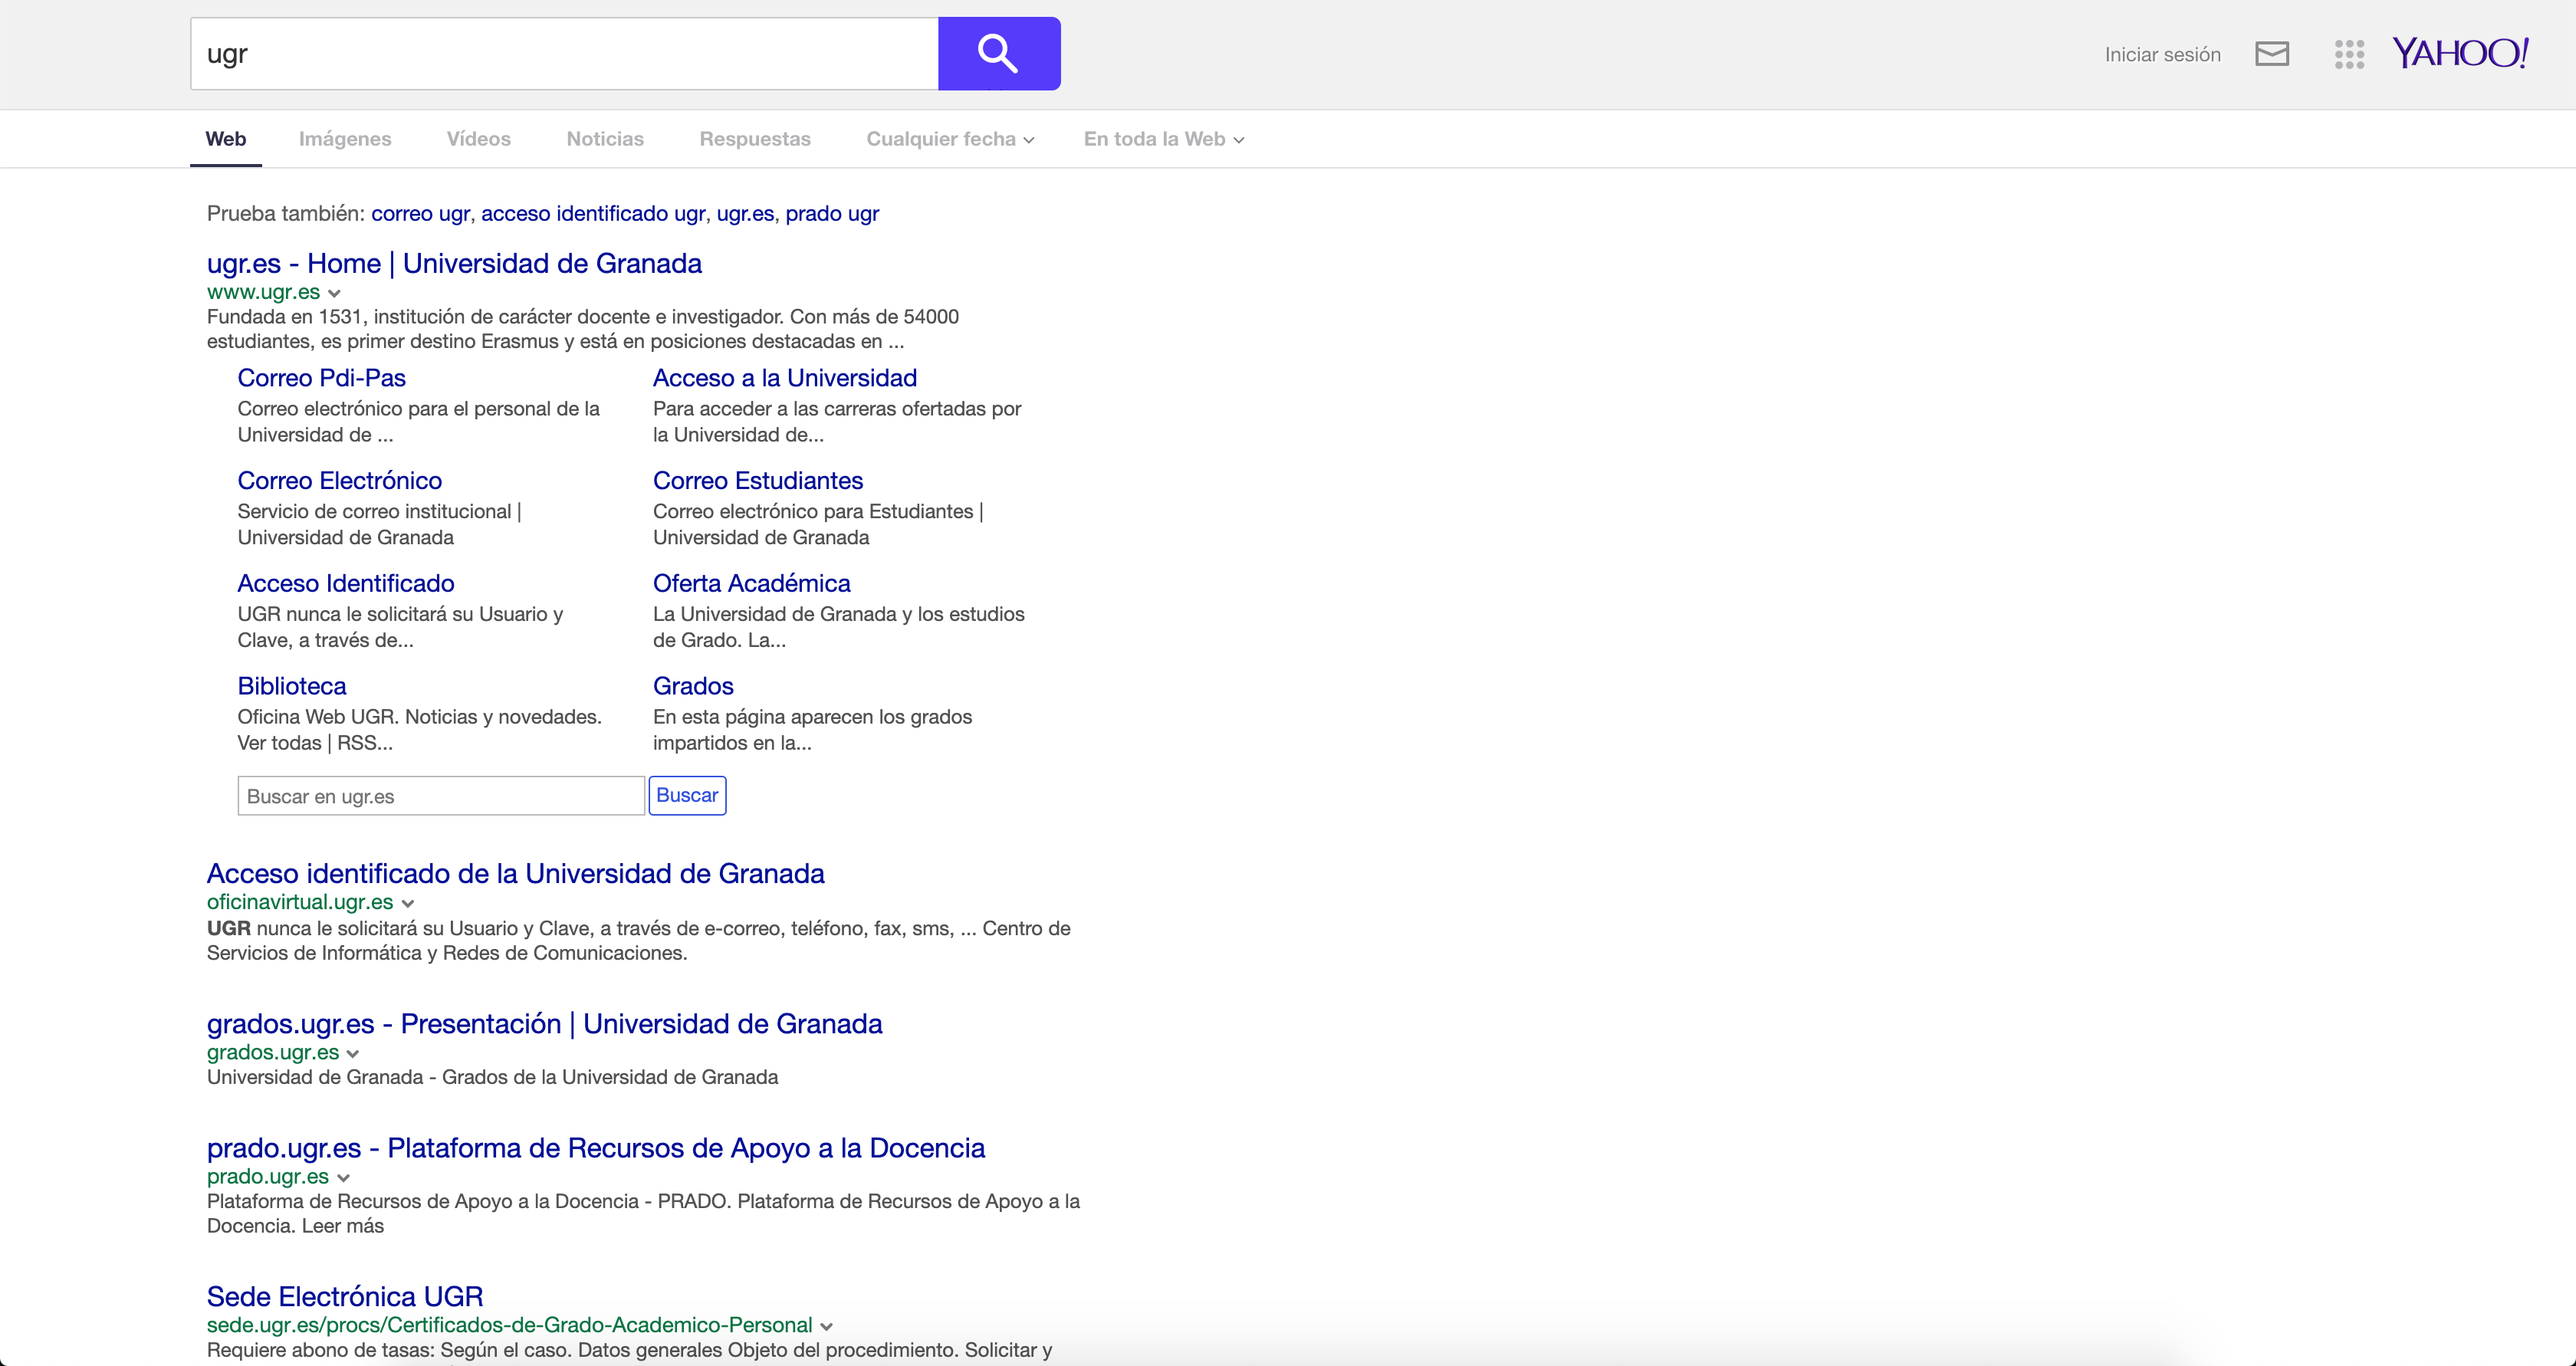
\includegraphics[height=6.7cm]{imagenes/capitulo3/yahoo-busqueda} % https://www.google.com/search/howsearchworks/
%	\caption{Búsqueda de ``ugr'' en Yahoo}
%	\label{yahoo-busqueda}
%\end{figure}

% Apuntes clase Jose
% COURSERA: La Web Semántica: Herramientas para la publicación y extracción efectiva de información en la Web
Por esta razón surge la Web Semántica, para proporcionar estructura al contenido semántico de las páginas Web, con la finalidad de que los contenidos puedan ser consumidos por máquinas de manera más eficiente. En el siguiente subapartado entramos en detalle en el concepto de Web Semántica.

\subsection{Concepto de Web Semántica} 

Para comprender que es la Web Semántica (\url{ www.semanticweb.org}), es necesario establecer los principios básicos sobre los que se asienta (figura \ref{fig:principio}). En el subapartado anterior se estableció el contexto en el que nace, a continuación se procede a explicar su definición. 

\begin{figure}[H]
	\centering
	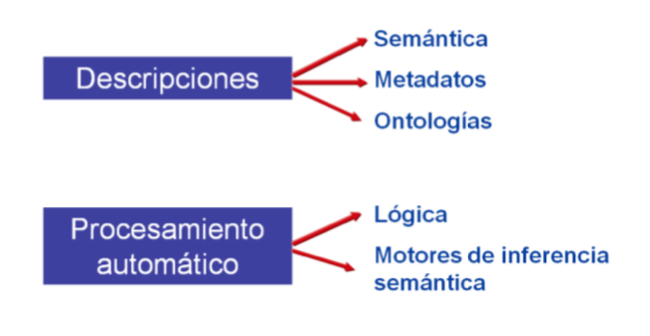
\includegraphics[width=0.56\linewidth]{imagenes/capitulo3/principio}
	\caption{Principios básicos de la Web Semántica \cite{aplicacion}}
	\label{fig:principio}
\end{figure}

La \textbf{Web Semántica} es una corriente promovida también por Tim Berners-Lee, cuyo fin es lograr que las máquinas puedan entender y, por tanto, utilizar lo que la Web contiene. De ahí que se haya tomado el término \textit{semántica}, que desde el punto de vista lingüístico ``\textit{es la disciplina que estudia el significado de los términos}'' \cite{cwb}. Esta idea surge a raíz de un artículo publicado por la revista \textit{Scientific American} en mayo de 2001, en donde Tim Berners-Lee propone una nueva forma de organizar el contenido en la Red para superar el problema de la heterogeneidad semántica y proporcionar a las computadoras contenidos Web significativos \cite{web-semantica-w3c, libro-gis}.\\



% EMPEZAMOS A DEFINIR - PRIMERA DEFINICIÓN LA OFICIAL (VER OTRAS DE LA LITERATURA)


% LA ONTOLOGÍA Y LA WEB SEMÁNTICA: RECOMENDACIONES DEL W3C. 
% http://www.fgcsic.es/lychnos/es_es/articulos/construyendo_una_web_semantica


% COURSERA: La Web Semántica: Herramientas para la publicación y extracción efectiva de información en la Web
% https://www.researchgate.net/publication/216537707_La_Web_semantica_y_las_tecnologias_del_lenguaje_humano
% https://disenowebakus.net/semantica-web.php
% LA ONTOLOGÍA Y LA WEB SEMÁNTICA: RECOMENDACIONES DEL W3C. 
% de descentralización, máxima facilidad de acceso y/o apertura al crecimiento
En palabras de Tim Berners-Lee \cite{researchgate}: ``\textit{La Web Semántica es una extensión de la actual Web en la que a la información disponible se le otorga un significado bien definido que permita a los ordenadores y a las personas trabajar en cooperación. Está basada en la idea de proporcionar en la Web datos definidos y enlazados, permitiendo que aplicaciones heterogéneas localicen, integren, razonen y reutilicen la información presente en la Web}''. Considerando la definición aquí aportada, la Web Semántica se manifiesta como una evolución de la actual Web, no una sustitución ya que mantiene sus características principales (descentralización, facilidad de acceso), en donde los ordenadores son capaces de interpretar los documentos; sin hacer uso de Inteligencia Artificial, ya que la semántica se encuentra en las páginas \cite{semantica-web}. \\

% OTRA DEFINICIÓN - W3C

% COURSERA: La Web Semántica: Herramientas para la publicación y extracción efectiva de información en la Web
% https://www.researchgate.net/publication/216537707_La_Web_semantica_y_las_tecnologias_del_lenguaje_humano
% https://disenowebakus.net/semantica-web.php
% LA ONTOLOGÍA Y LA WEB SEMÁNTICA: RECOMENDACIONES DEL W3C. 
% https://disenowebakus.net/semantica-web.php
Pero, \textit{¿cómo se traduce lo que acabamos de definir a la práctica?} En la práctica, la Web Semántica es un conjunto de recomendaciones\footnote{Una recomendación es una descripción formal de una tecnología que debe ser utilizada por todos.} desarrolladas por el \textbf{World Wide Web Consortium}\textbf{ (W3C) }que es el organismo encargado de velar por la normalización en Internet y dictar los distintos estándares para la Web. El objetivo principal de este organismo reside en ``\textit{guiar a la Web hacia su máximo potencial mediante el desarrollo de protocolos y pautas comunes que promuevan su evolución y garanticen su interactividad}’’ \cite{coursera, web-semantica-w3c}. Dentro de la página oficial del W3C (\url{https://www.w3.org}), podemos encontrar otra definición para la Web Semántica: ``\textit{La Web Semántica es la representación de datos en la Web. Es un esfuerzo colaborativo liderado por W3C con la participación de un gran número de investigadores y socios industriales. Se basa en el uso de RDF, que integra una gran variedad de aplicaciones mediante el uso de XML, para la sintaxis y el uso de URLs para su identificación}'' \cite{semantica-web}. Considerando la definición aquí expuesta, los términos mencionados se escapan de los conocimientos aprendidos hasta ahora, en donde las tecnologías nombradas serán tratadas en sucesivos apartados, ya que la W3C recomienda el uso de RDF (\textit{Resource Description Framework}) y OWL (\textit{Ontology Web Language}) para la construcción de la Web Semántica.\\

% tesis
% INTRODUCCIÓN A LA WEB SEMÁNTICA: REALIDADES Y PERSPECTIVAS.
% COURSERA: La Web Semántica: Herramientas para la publicación y extracción efectiva de información en la Web
De igual manera, nos encontramos a lo largo de la literatura más definiciones de Web Semántica, si bien todas guardan un nexo en común y es el de dotar de mayor significado a la Web actual a través de lenguajes universales que resuelvan los problemas ocasionados por una Web carente de semántica en la que a veces el acceso a la información se convierte en una tarea difícil \cite{introduccion}. Para ello, se desarrollan y usan lenguajes que facilitan la introducción en la Web de contenido legible por las máquinas \cite{tesis}. Entonces, \textit{¿cuáles son los requisitos esenciales para que una Web de datos pueda ser accedida y entendida tanto por ordenadores como por personas?} \cite{coursera}:

\begin{enumerate}
	\item Se necesita disponer de un l\textbf{enguaje que permita especificar los recursos de la Web y las relaciones que existen entre ellos}. Con esto, lo que se pretende es desarollar una Web más cohesionada en donde sea más fácil localizar, compartir e integrar información para sacar un mayor partido a los recursos disposibles. Para conseguir este objetivo es necesario que un sistema automático sea capaz de sacar sus propias conclusiones respecto a las búsquedas realizadas.
	
	\item Se necesita poder consultar esos datos mediante aplicaciones computacionales. Para ello es necesario disponer de un \textbf{lenguaje para describir consultas procesables por un computador} para su entendimiento y ser capaz de sacar conclusiones a partir de los datos de manera automática. Con esto se pretende explorar la Web de forma más automática y obtener resultados más enfocados.
\end{enumerate}

En la figura \ref{fig:pasowa-ws} se muestra como puede llegarse al conocimiento, articulado en las ontologías, con la aplicación de técnicas de extracción de información en los documentos expresados en lenguaje natural de la Web actual. A partir de aquí pueden crearse contenidos con la arquitectura propia de la Web Semántica y generar directamente contenidos en lenguaje natural en diferentes idiomas. Además, se recoge la necesidad de que la extracción de información de los textos debe estar vinculada directamente a las ontologías, ya que la Web Semántica necesita que la información tenga una estructura jerárquica para poder realizar las inferencias \cite{researchgate}.

\begin{figure}[H]
	\centering
	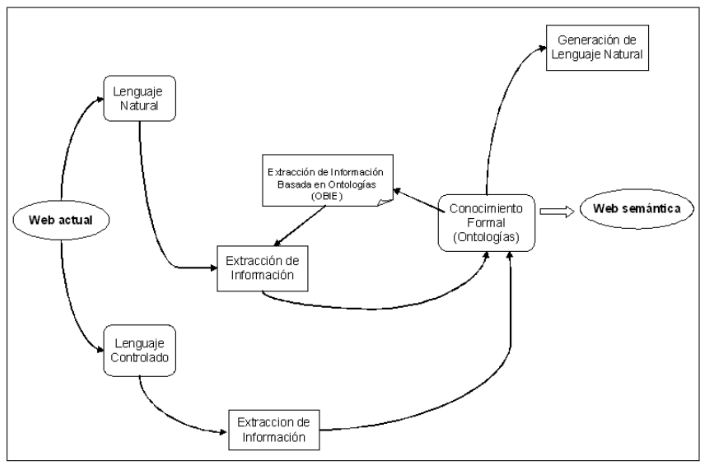
\includegraphics[width=0.7\linewidth]{imagenes/capitulo3/pasoWA-WS}
	\caption{Paso de la Web actual a la Web Semántica \cite{researchgate}}
	\label{fig:pasowa-ws}
\end{figure}

\begin{figure}[H]
	\centering
	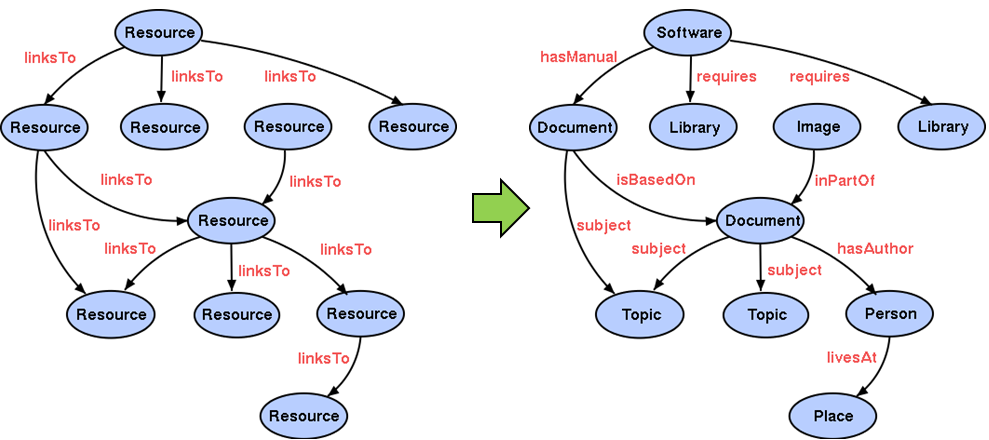
\includegraphics[height=5.60cm]{imagenes/capitulo3/web-actual-web-semantica.png}
	\caption{Web Sintáctica vs. Web Semántica \cite{imagen-diferencia}}
	\label{wa-ws}
\end{figure}

% https://www.researchgate.net/publication/216537707_La_Web_semantica_y_las_tecnologias_del_lenguaje_humano
A partir de los conceptos explicados hasta ahora, la implantación de la Web Semántica frente a la actual Web supone un cambio de paradigma, ya que tiene que pasarse de una Web basada y creada en lenguaje natural a una Web estructurada y organizada, en donde los contenidos etiquetados semánticamente serán el elemento principal \cite{researchgate}. En la figura \ref{wa-ws} podemos ver la diferencia que hay entre ambos tipos de Web. Se observa como el esquema de la izquierda, el de la actual Web, está basado en los hipervínculos que nos permiten ir saltando de una página Web a otra, mientras que en la Web Semántica (esquema de la derecha) disponemos de información relevante.\\



% https://www.makeuseof.com/tag/top-7-semantic-search-engines-alternative-google-search/
% http://swoogle.umbc.edu/2006/ no funciona 
Por otro lado, para comprender los conceptos hasta aquí tratados, vamos a ver un ejemplo de buscador semántico. En Internet existen muchos buscadores de este tipo, de entre todas las posibilidades revisadas \cite{buscadores-semanticos} nos hemos quedado con dos: \textit{Swoogle} (\url{http://swoogle.umbc.edu/2006/}) y \textit{DuckDuckGo} (\url{https://duckduckgo.com/?t=h_}), pero debido a que el primero no ha funcionado, hemos hecho una pequeña demostración con el segundo. \textbf{DuckDuckGo} es un motor de búsqueda semántico rico en funciones que tiene innumerables razones para dejar atrás a Google. Respecto a las búsquedas, podemos diferenciar en una búsqueda clásica, búsqueda de información y/o compras, entre otros. Si se busca un término que tiene más de un significado, nos da la oportunidad de elegir lo que estamos buscando originalmente, con sus distintos resultados o significados. 

\begin{figure}[H]
	\centering
	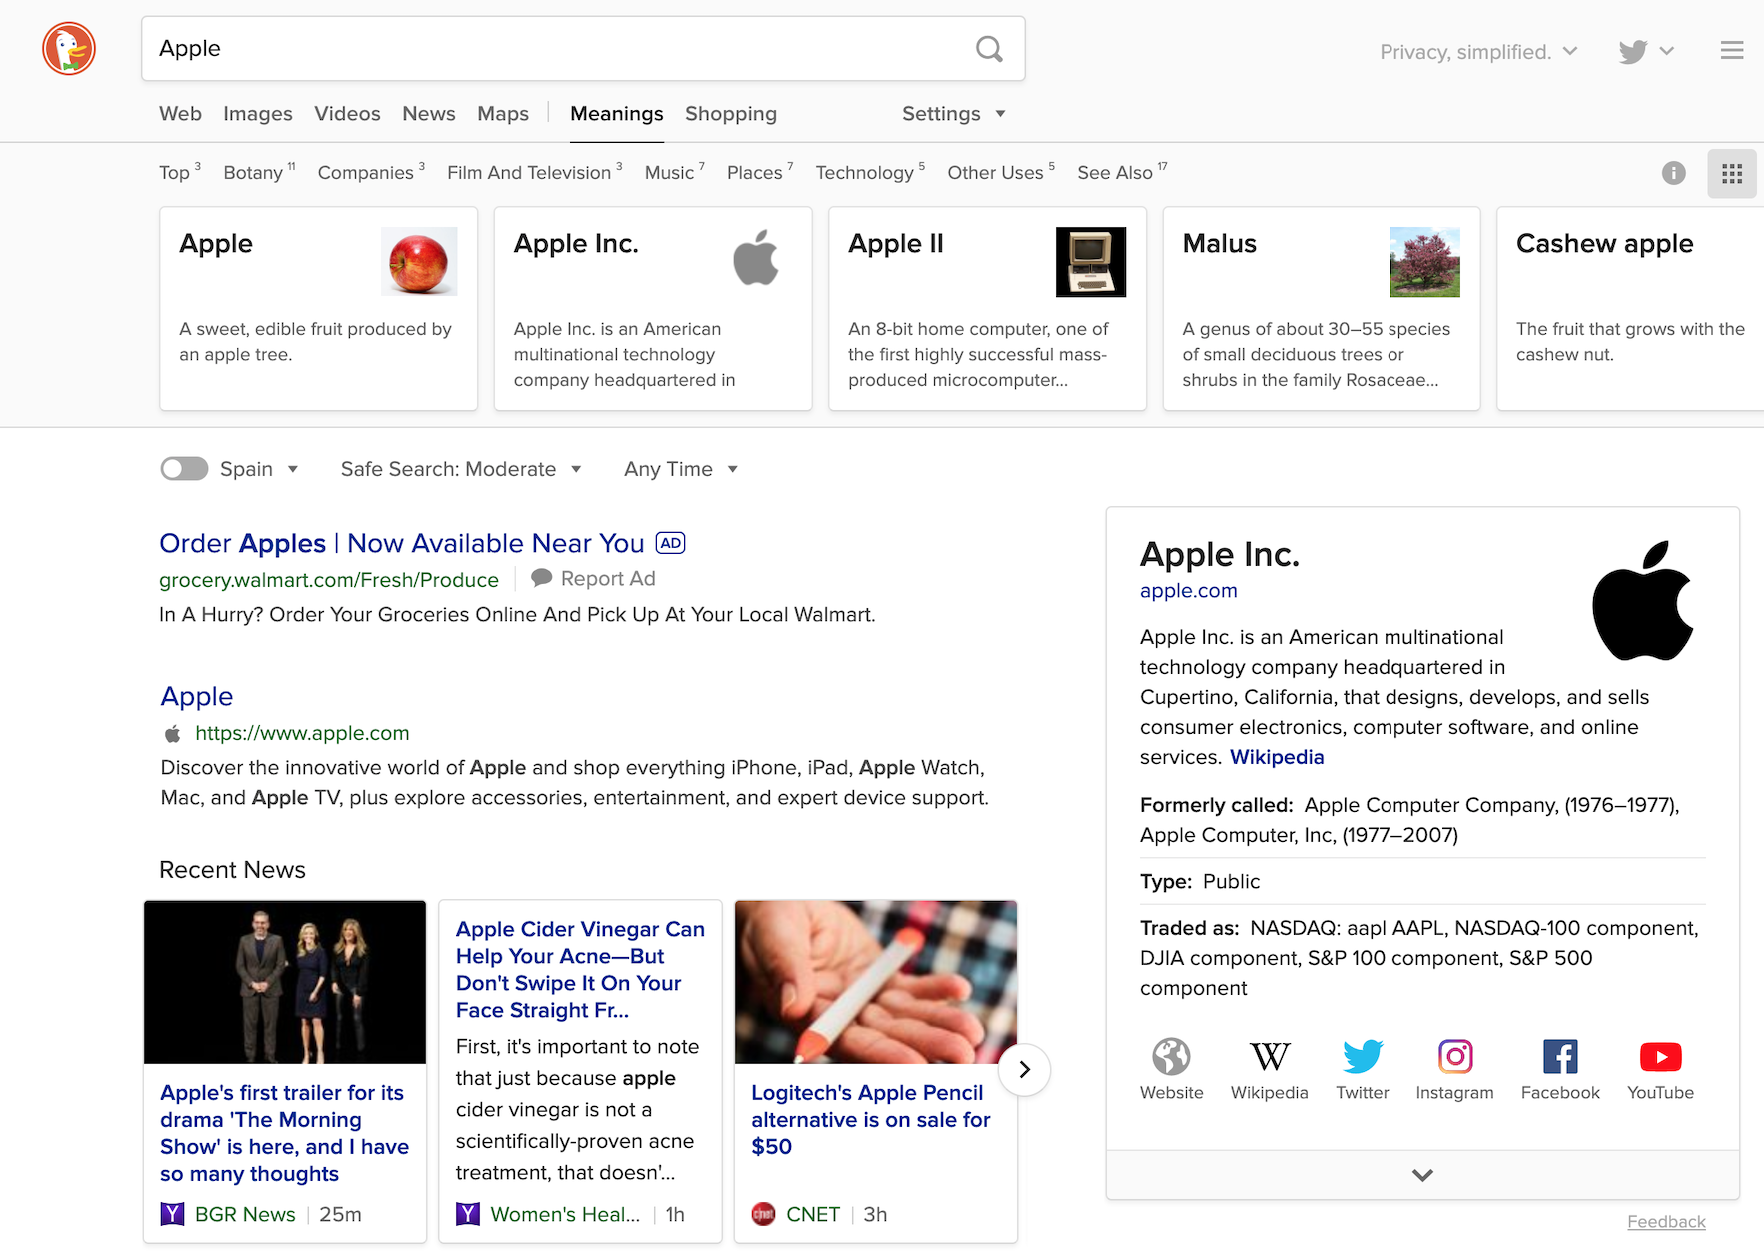
\includegraphics[height=9.cm]{imagenes/capitulo3/duck21}
	\caption{Búsqueda semántica de ``Apple'' en DuckDuckGo}
	\label{busqueda-semantica}
\end{figure}

Por ejemplo, la búsqueda del término \textit{Apple}, en un navegador con idioma inglés, ofrece una larga lista de posibles significados, entre los que podemos destacar principalmente la fruta y la empresa tecnológica, a parte de muchos otros. Además, los clasifica en categorías, como se puede observar en la figura \ref{busqueda-semantica}. Sin embargo, la búsqueda para el término \textit{Apple} en un buscador sintáctico como puede ser Google, nos ofrece de primeras sólo la empresa tecnológica, ya que debido a estadísticas se obtiene que esa es la simlitud con mayor porcentaje para mostrar antes que otros resultados (figura \ref{busqueda-sintactica}).

\begin{figure}[H]
	\centering
	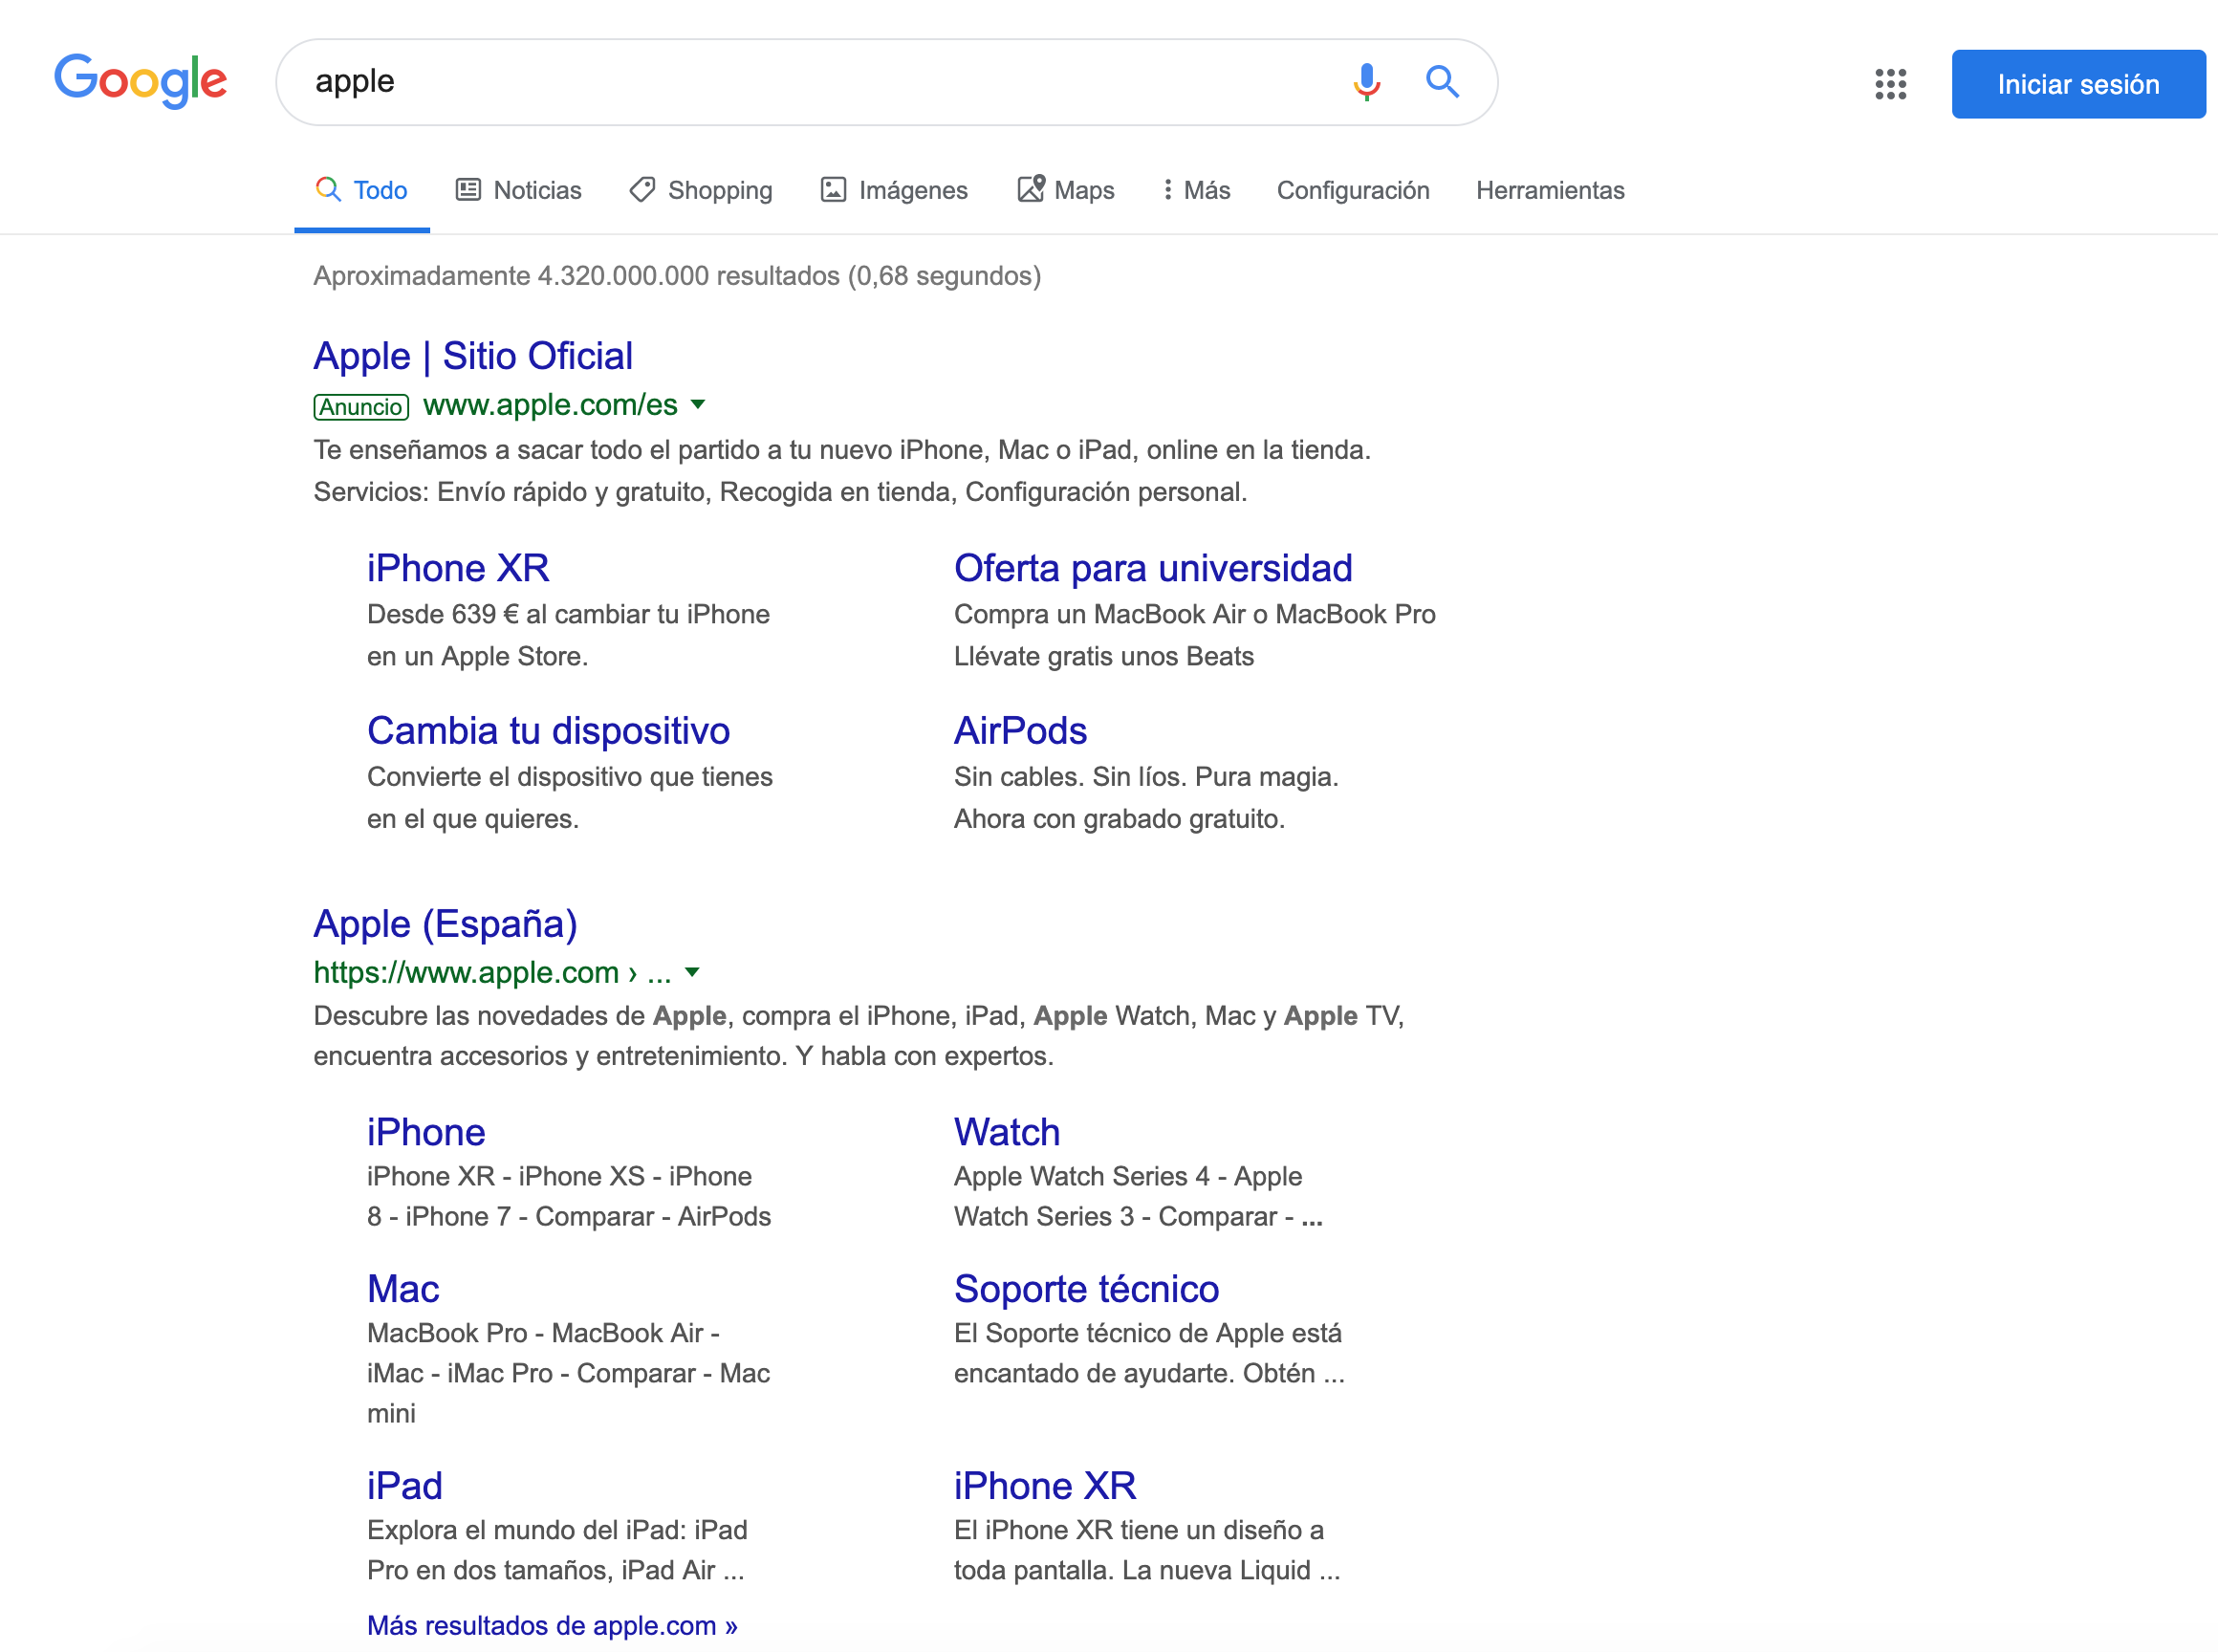
\includegraphics[height=9.4cm]{imagenes/capitulo3/apple}
	\caption{Búsqueda clásica de ``Apple'' en Google}
	\label{busqueda-sintactica}
\end{figure}

%\begin{figure}[H]
%	\centering
%	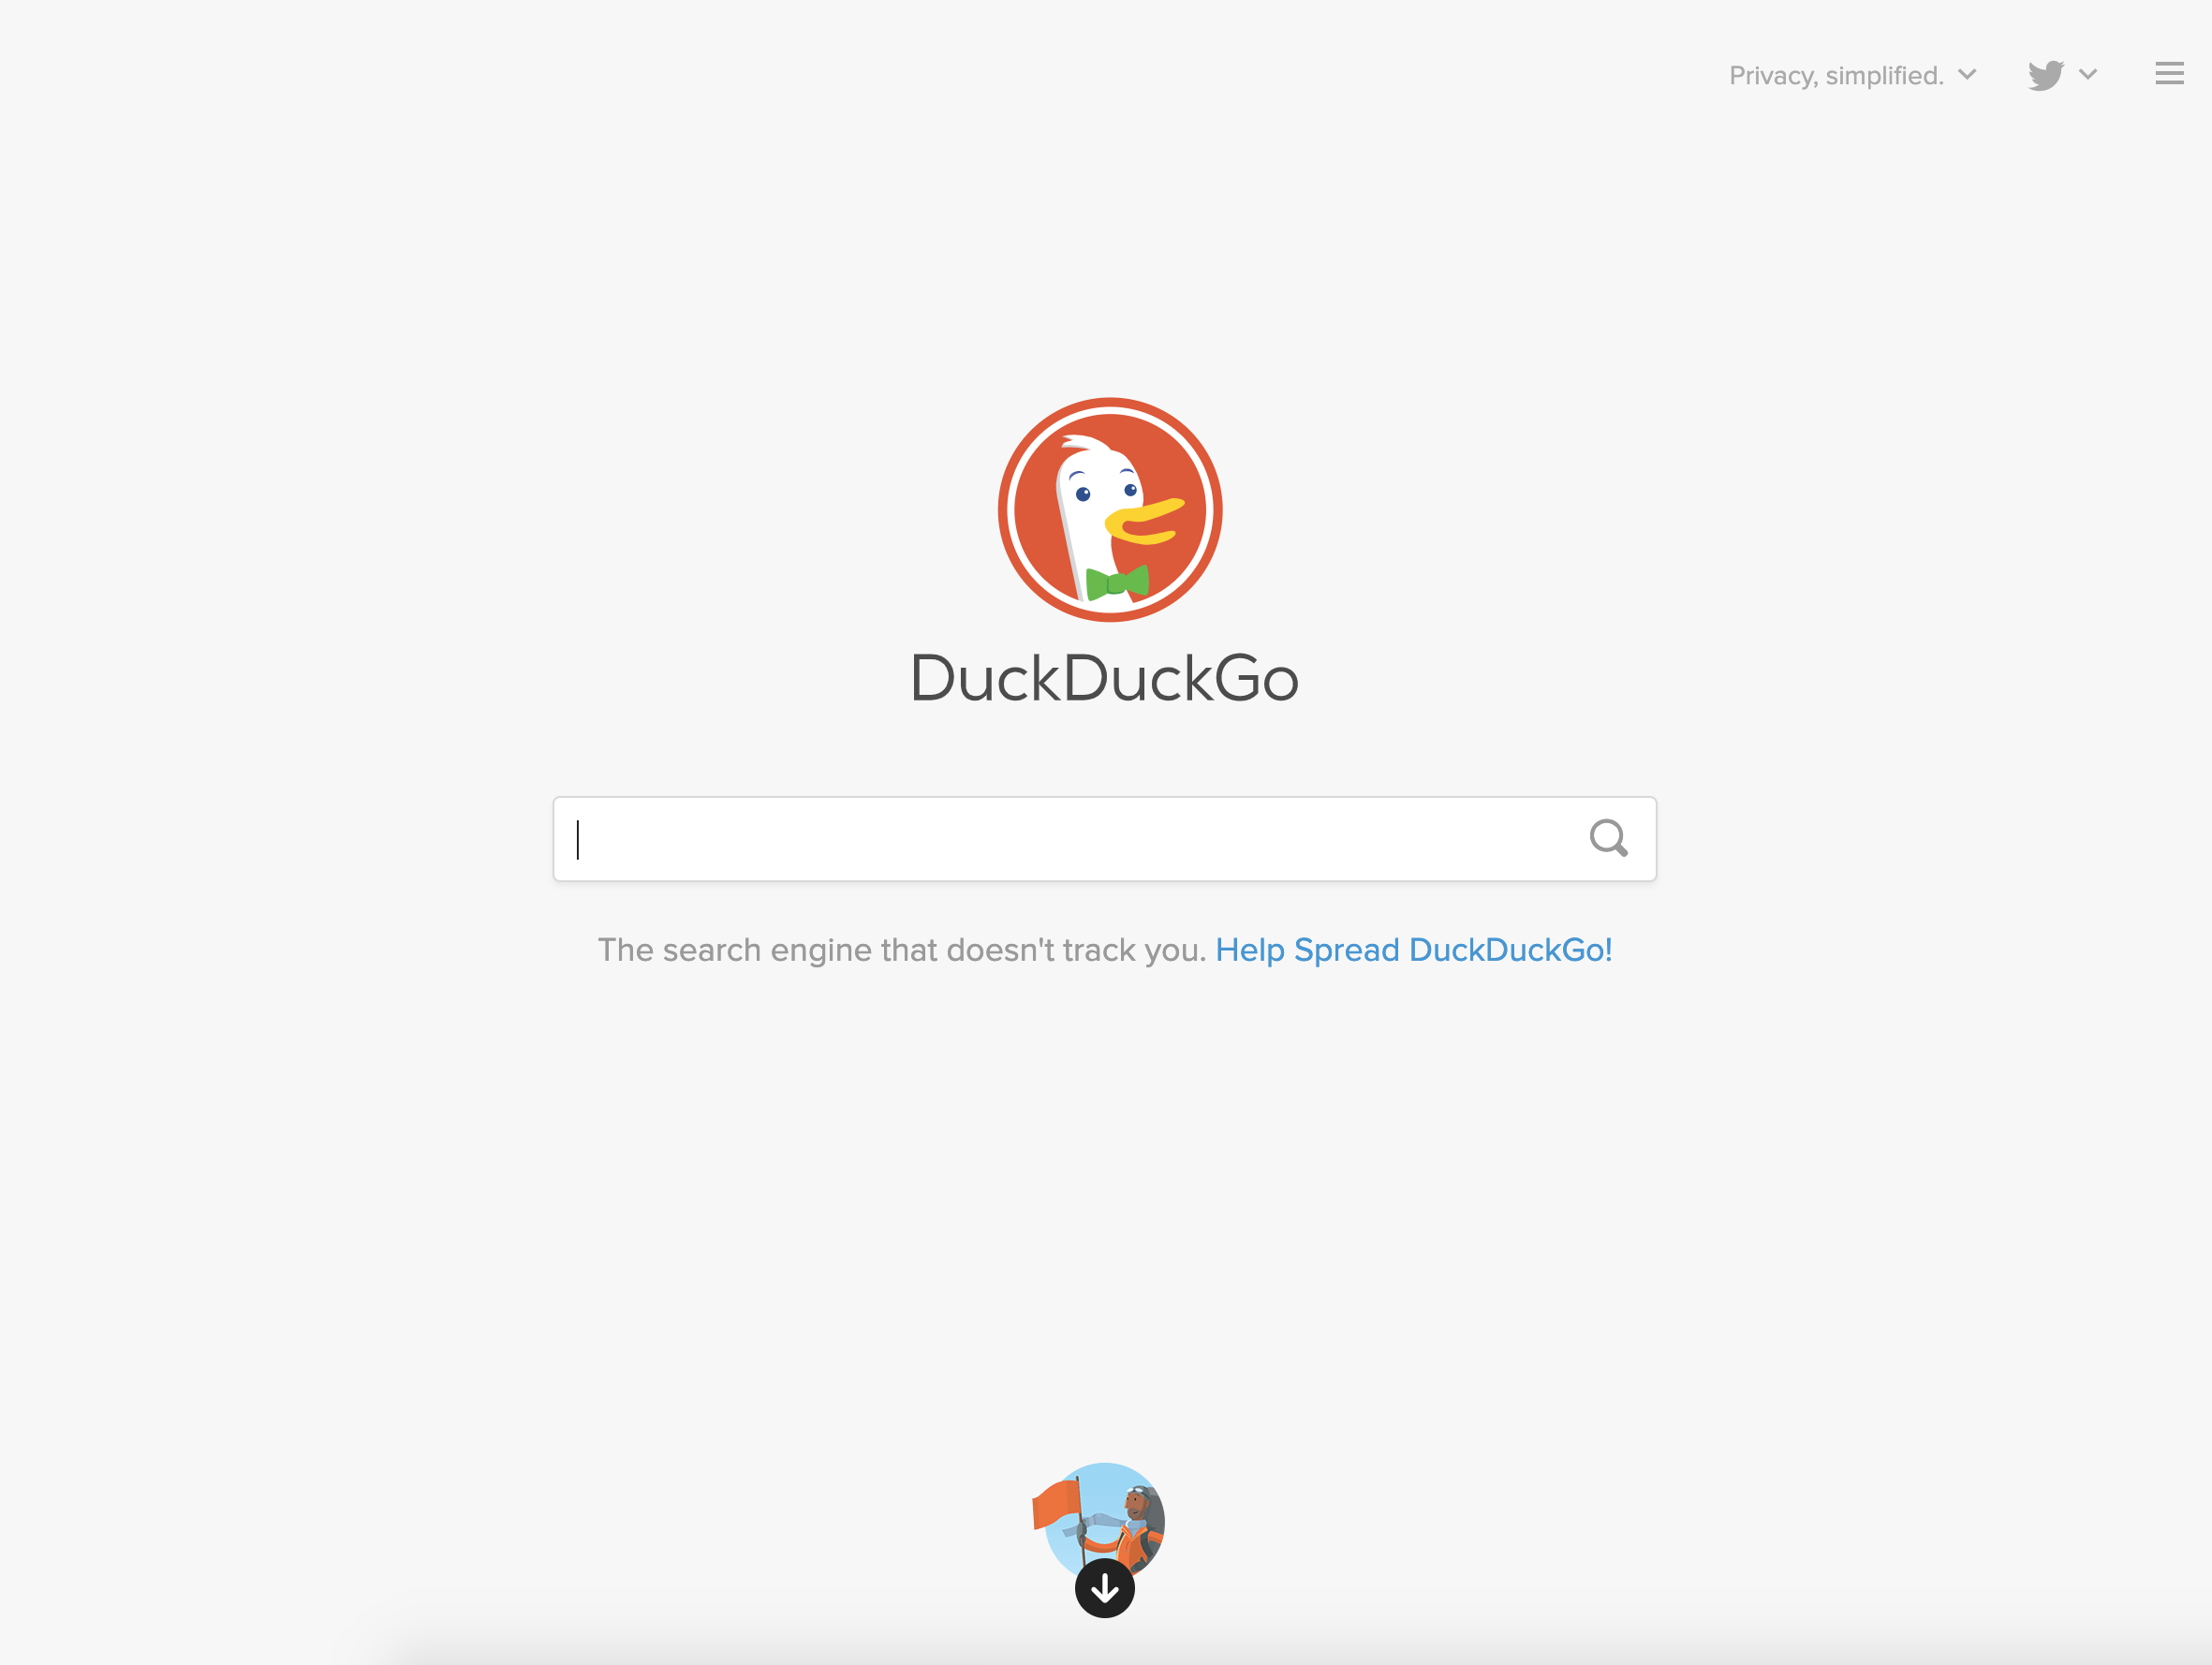
\includegraphics[height=8.5cm]{imagenes/capitulo3/duck1}
%	\caption{DuckDuckGo}
%	\label{DuckDuckGo}
%\end{figure}

Por tanto, después de haber analizado este ejemplo podemos concluir que la mayoría de los contenidos de la Web de hoy en día están diseñados para que los humanos los lean, no para que los programas de software procesen la semántica de manera significativa. Es por eso que nace la Web Semántica, para llevar estructuras a los contenidos significativos de las páginas Web y permitir que los programas de software procesen y comprendan los datos en las páginas. En donde, dichas tecnologías tratan de aportar información extra a los recursos Web, proporcionando contenidos con significado que permitan mejorar la interoperabilidad entre los sistemas informáticos \cite{aplicacion}. A través de la Web Semántica, los programas de software pueden usar colecciones estructuradas de información y conjuntos de reglas de inferencia para realizar razonamientos automatizados \cite{libro-gis}. \\

Con esto hemos terminado de definir el concepto de Web Semántica, a continuación se explican las capas que componen su arquitectura, tecnologías usadas en la prueba de concepto que se verá en el siguiente capítulo.



\section{Arquitectura de la Web Semántica}

% ARQUITECTURA 
% Capas de la Web Semántica

% https://www.researchgate.net/publication/216537707_La_Web_semantica_y_las_tecnologias_del_lenguaje_humano
\textit{¿Cuáles son los estándares para la Web Semántica?} En la figura \ref{fig:arquitectura1} se muestra la arquitectura de la Web Semántica tal y como la definió Berners-Lee. Se trata de una estructura de capas, donde cada nivel resulta un requisito previo para el siguiente \cite{researchgate}:

\begin{figure}[H]
	\centering
	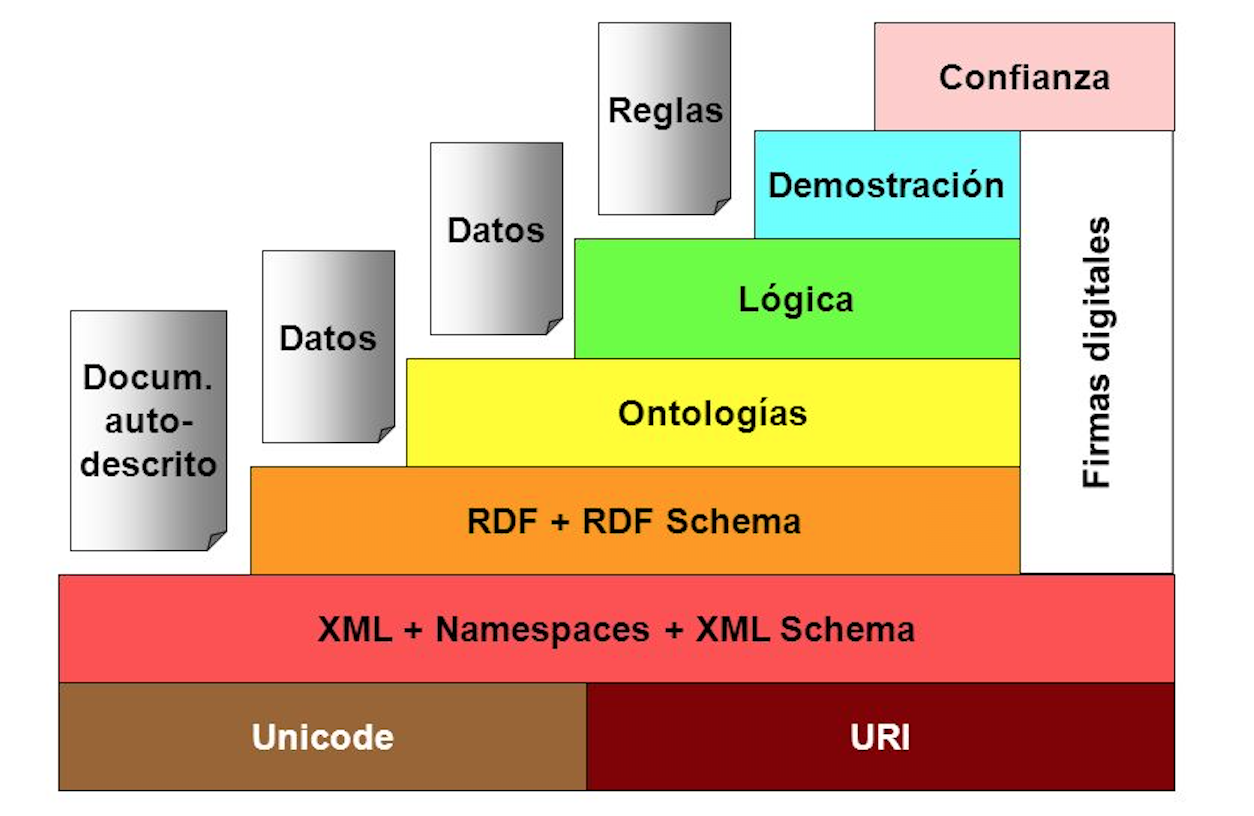
\includegraphics[width=0.65\linewidth]{imagenes/capitulo3/arquitectura1} 
	\caption{Modelo multicapa de la Web Semántica \cite{researchgate}}
	\label{fig:arquitectura1}
\end{figure}


% https://www.researchgate.net/publication/216537707_La_Web_semantica_y_las_tecnologias_del_lenguaje_humano
\begin{enumerate}
	\item \textbf{Unicode, URI, XML y RDF}: los tres primeros niveles hacen referencia a la base y los estándares en los que se sustenta su desarrollo, ya que permiten convertir la Web en una infraestructura global para compartir y reutilizar datos y documentos entre diferentes usuarios.
	
	\item \textbf{Ontologías}: capa donde reside el contenido semántico del sistema. 
	
	\item \textbf{Lógica}: en esta capa a partir de la estructura semántica generada con las ontologías y los metadatos, se realizan las inferencias lógicas; sin embargo, actúan como freno para la Web Semántica ya que comportan una infraestructura que actualmente es difícil de realizar a gran escala. 
	
	\item \textbf{Seguridad y Confianza}: los agentes deben ser escépticos de la información obtenida, y contrastar minuciosamente las distintas fuentes; podrán utilizar la firma digital para verificar que la fuente es confiable. 
	%las dos últimas capas más rápidas en implantarse, ya que la confianza y la seguridad son elementos clave de cualquier arquitectura, y se podrá usar la firma digital para verificar la fuente.
\end{enumerate}



La figura \ref{fig:arquitectura1} no es la única forma de representación de las capas de la arquitectura para la Web Semántica, sino que a lo largo de los años han surgido otros tipos de representaciones similares. En el presente trabajo nos vamos a centrar en otro esquema (figura \ref{fig:arquitectura2}), el cual ha sido explicado en los cursos a los que he asistido durante este año. Así que a partir del esquema de la figura \ref{fig:arquitectura2}, vamos a describir las tecnologías o capas de carácter importante que se utilizan durante el desarrollo del presente trabajo: URI/IRI, XML, RDF, RDF Schema, Ontología (OWL) y SPARQL (GeoSPARQL).

\begin{figure}[H]
	\centering
	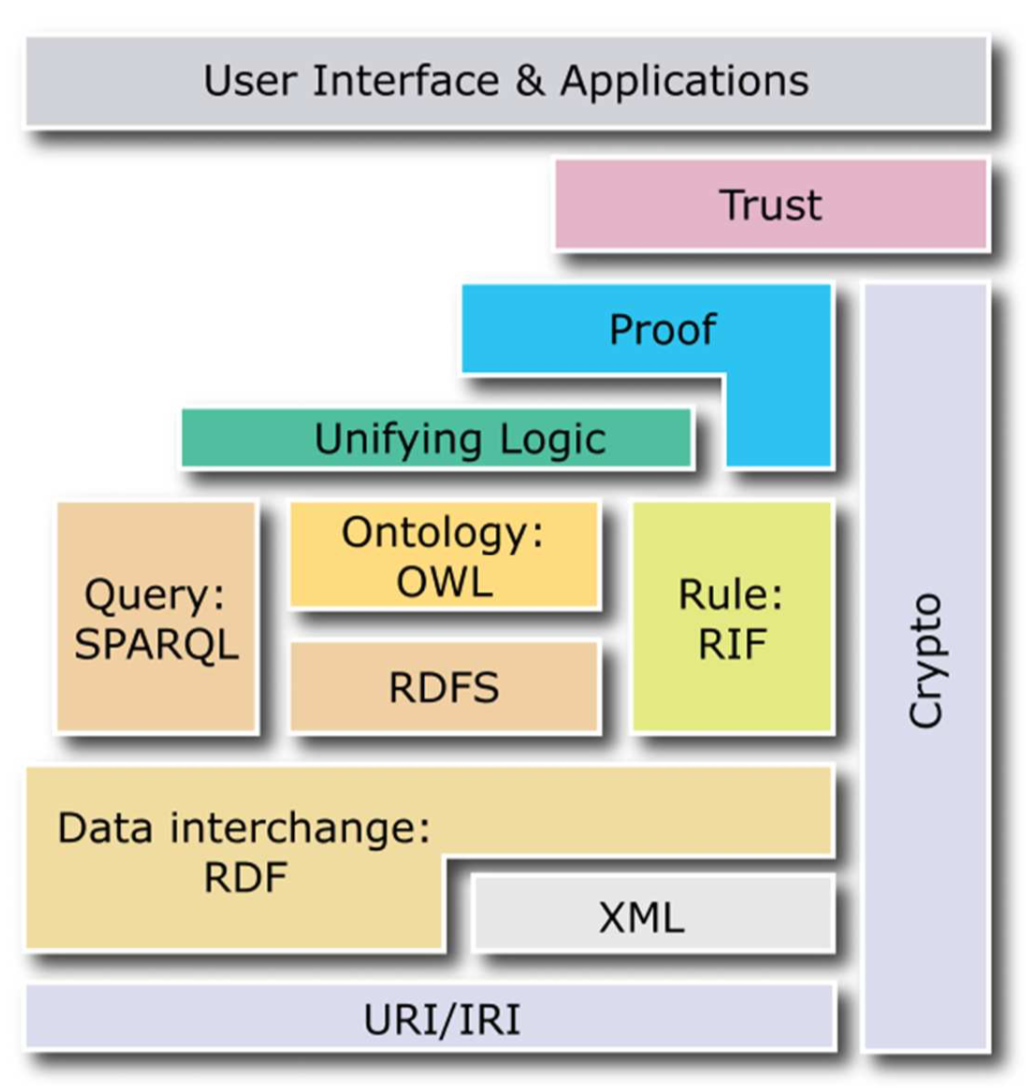
\includegraphics[width=0.52\linewidth]{imagenes/capitulo3/arquitectura2}
	\caption{Estructura de la Web Semántica \cite{apuntes-clase-jose}}
	\label{fig:arquitectura2}
\end{figure}


% En este curso nos vamos a centrar en cuatro de estos componentes de esta pirámide que están marcados con colores. En primer lugar vamos a ver RDF, que es el lenguaje básico para especificar recursos de la web y sus relaciones, RDFS que nos permite decir un poco más vamos a hablar de este vocabulario, SPARQL que es este lenguaje de consulta que nos permite extraer información desde la web y finalmente OWL o este lenguaje que nos permite identificar ontologías.

\subsection{URI/IRI}

URI/IRI son los identificadores de la Web (figura \ref{fig:250px-irivenndiagramm}). Son el primer elemento necesario para el acceso a los recursos de la Web, los cuales pueden ser identificados unívocamente en cualquier idioma, a través del uso de Unicode e identificadores URI \cite{aplicacion}. El \textbf{URI} (\textit{\textbf{Uniform Resource Identifier}}) es una secuencia compacta de caracteres que identifican un recurso abstracto o físico que no tiene porqué existir en la Web. En la tabla \ref{uris} se observan algunos ejemplos de URIs \cite{uri}.


\begin{table}[H]
	\caption{Ejemplos de URIs}
	\label{uris}
	\centering
	\begin{tabular}{|m{5.6cm}|m{5.6cm}|}
		\rowcolor[HTML]{EFEFEF} 
		\hline
		Ejemplo & Descripción \\ \hline
		\url{ftp://ftp.is.co.za/rfc/rfc1808.txt} & Esquema FTP para servicios de protocolo de transferencia de archivos\\ \hline
		%\url{http://www.math.uio.no/faq/compression-faq/part1.html} & esquema http para servicios de protocolo de transferencia de hipertexto\\ \hline
		\url{mailto:mduerst@ifi.unizh.ch} & Esquema MAILTO para direcciones de correo electrónico \\ \hline
		\url{telnet://melvyl.ucop.edu/} & Esquema TELNET para servicios interactivos a través del protocolo TELNET\\ \hline
	\end{tabular}
\end{table}

\begin{figure}[H]
	\centering
	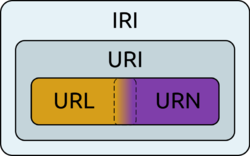
\includegraphics[width=0.28\linewidth]{imagenes/capitulo3/URI}
	\caption{Conjunto que englobas las IRI \cite{imagen-iri}}
	\label{fig:250px-irivenndiagramm}
\end{figure}

El \textbf{IRI} (\textit{\textbf{International Resource Identifier}}) se puede utilizar para encontrar diferentes tipos de recursos, como documentos, personas, objetos físicos y conceptos abstractos. Las URL que usamos como direcciones Web son una forma de IRI que sí existen en la Web. Además el IRI nace como complemento del URI, debido a que los IRI son identificadores globales y los usuarios pueden reutilizarlos para identificar lo mismo \cite{libro-gis}.


%Son los identificadores de la Web, la URi no tiene porqué existir en la Web www.ugr.es/jsamos es existe es una URL, la URI no tiebe porque 

%Lo más genrico con los URI

% https://www.ietf.org/rfc/rfc3986.txt
% https://www.ietf.org/rfc/rfc3986.txt
%Un identificador uniforme de recursos (URI) es una secuencia compacta de caracteres que identifican un recurso abstracto o físico. Esta
%La especificación define la sintaxis genérica de URI y un proceso para resolviendo referencias de URI que podrían estar en forma relativa, junto con directrices y consideraciones de seguridad para el uso de URI en el Internet. La sintaxis de URI define una gramática que es un superconjunto de todos URI válidos, lo que permite una implementación para analizar los componentes comunes de una referencia URI sin conocer los requisitos específicos del esquema de cada posible identificador. Esta especificación no define un gramática generativa para URIs; esa tarea la realiza el individuo especificaciones de cada esquema URI.


% https://www.ietf.org/rfc/rfc3986.txt
%Este documento define un nuevo elemento de protocolo, el Internacionalizado Identificador de recursos (IRI), como complemento del recurso uniforme Identificador (URI). Un IRI es una secuencia de caracteres de Juego de caracteres universal (Unicode / ISO 10646). Un mapeo de IRIs a Se definen URI, lo que significa que se pueden usar IRI en lugar de URI, en su caso, para identificar recursos.

%Se eligió el enfoque de definir un nuevo elemento de protocolo en lugar de extender o cambiar la definición de URI. Esto se hizo en orden para permitir una distinción clara y evitar incompatibilidades con software existente Se proporcionan pautas para el uso y despliegue de IRI en varios protocolos, formatos y software componentes que actualmente tratan con URI.

% https://www.ietf.org/rfc/rfc3986.txt
%Los IRI están destinados a reemplazar los URI en la identificación de recursos para
%protocolos, formatos y componentes de software que usan un UCS
%repertorio de personajes. Es posible que estos protocolos y componentes nunca necesiten
%para usar los URI directamente, especialmente cuando se usa el identificador de recursos
%simplemente con fines de identificación. Sin embargo, cuando el recurso
%identificador se utiliza para la recuperación de recursos, en muchos casos
%necesario para determinar el URI asociado, porque actualmente la mayoría
%Los mecanismos de recuperación solo se definen para los URI. En este caso, IRI
%puede servir como elementos de presentación para elementos de protocolo URI. Un
%ejemplo sería una barra de direcciones en un agente de usuario web. (Adicional
%La justificación se da en la sección 3.1.)


%A URI can be further classified as a locator, a name, or both.  The
%term "Uniform Resource Locator" (URL) refers to the subset of URIs
%that, in addition to identifying a resource, provide a means of
%locating the resource by describing its primary access mechanism
%(e.g., its network "location").  The term "Uniform Resource Name"
%(URN) has been used historically to refer to both URIs under the
%"urn" scheme [RFC2141], which are required to remain globally unique
%and persistent even when the resource ceases to exist or becomes
%unavailable, and to any other URI with the properties of a name.

%An individual scheme does not have to be classified as being just one
%of "name" or "locator".  Instances of URIs from any given scheme may
%have the characteristics of names or locators or both, often
%depending on the persistence and care in the assignment of
%identifiers by the naming authority, rather than on any quality of
%the scheme.  Future specifications and related documentation should
%use the general term "URI" rather than the more restrictive terms
%"URL" and "URN" [RFC3305].



\subsection{XML} % Extensible Markup Language (XML). 

% https://www.w3.org/XML/
%HTML es muy limitado

%Orientado a la presentación de los datos.
%No permite la descripción de los datos. 􏰁No es extensible.

%XML es necesario pero no suficiente
%Es un lenguaje de marcado para describir datos estructurados.
%No tiene etiquetas predefinidas – nosotros definimos las etiquetas.
%XML Schema describe la estructura – El validador.
%El problema es que las etiquetas no tienen un significado compartido.
%XML modela documentos, y el mundo real no es un documento, sino una red de relaciones y objetos.
%XML estandariza formato no significado.

%Para la descripción sintáctica de los recursos se utiliza XML y XML-Schema como estándares de base, pero es necesario utilizar lenguajes que permitan imponer restricciones semánticas para descripciones completas.


\textbf{XML (\textit{Extensible Markup Language})} es un lenguaje de marcas, derivado de SGML\footnote{SGML (\textit{Standard Generalized Markup Language}) es un lenguaje para marcar y describir documentos con independencia total del hardware y software utilizados.}, pensado para ser utilizado en el entorno Web y para ser usado en la descripción sintáctica de los recursos, es decir, es la herramienta utilizada para estructurar y presentar los contenidos Web (figura \ref{fig:xml}). No obstante, ofrece una capacidad limitada para expresar semántica (no tiene etiquetas predefinidas), por lo que es necesario utilizar lenguajes que permitan imponer restricciones semánticas para descripciones completas \cite{aplicacion}.

\begin{figure}[H]
	\centering
	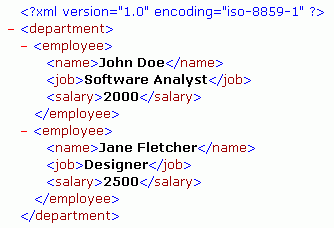
\includegraphics[width=0.45\linewidth]{imagenes/capitulo3/xml}
	\caption{Ejemplo de XML \cite{imagen-xml}}
	\label{fig:xml}
\end{figure}


%\begin{figure}[H]
%	\centering
%	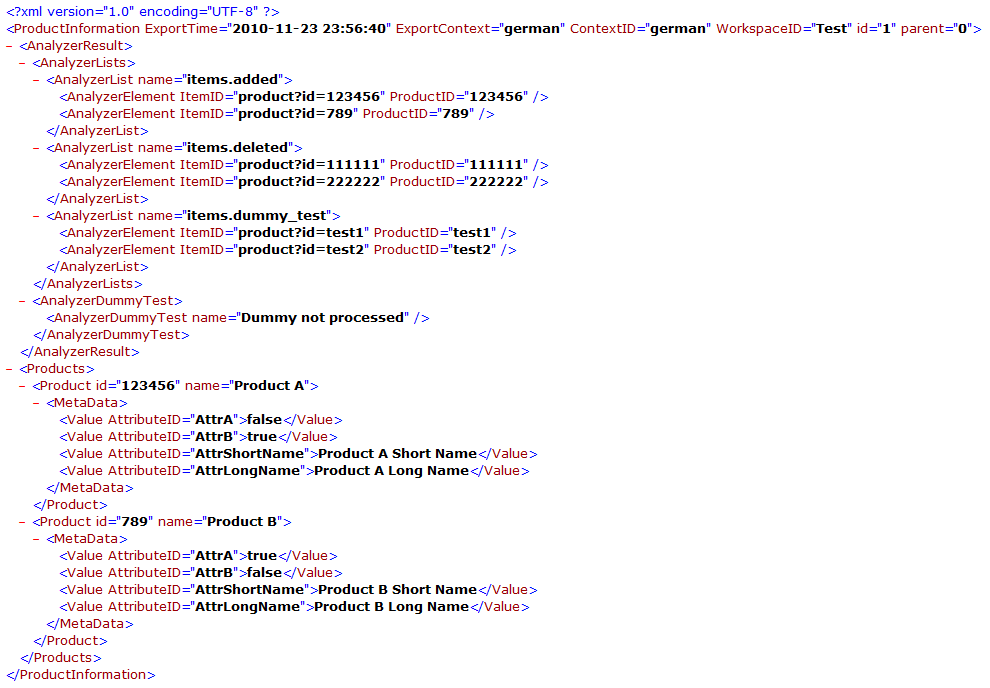
\includegraphics[width=0.92\linewidth]{imagenes/capitulo3/1*kwUlHDYmt_TaWK7ZefEE8Q}
%	\caption{Ejemplo de XML}
%	\label{fig:1kwulhdymttawk7zefee8q}
%\end{figure}



%Por tanto, XML responde a la necesidad de representar sintácticamente el modelo planteado por RDF para archivos legibles por ordenador.

% Por eso, se entiende que RDF es a la Semántica lo que XML es a la Sintaxis. Gracias a RDF se expresan afirmaciones y mediante su lenguaje de base XML se define la estructura de tales afirmaciones. Por tanto, XML responde a la necesidad de representar sintácticamente el modelo planteado por RDF para archivos legibles por ordenador.


%Para la descripción sintáctica de los recursos se utiliza XML y XML-Schema como estándares de base, pero es necesario utilizar lenguajes que permitan imponer restricciones semánticas para descripciones completas.

% Originalmente fue diseñado para enfrentar los desafíos de la publicación electrónica a gran escala, XML también desempeña un papel cada vez más importante en el intercambio de una amplia variedad de datos en la Web y en otros lugares.

%Esta página describe el trabajo que se está realizando en W3C dentro de la Actividad XML y cómo está estructurado. El trabajo en el W3C se lleva a cabo en grupos de trabajo. Los grupos de trabajo dentro de la actividad XML se enumeran a continuación, junto con enlaces a sus páginas web individuales.

%Puede encontrar y descargar especificaciones técnicas formales aquí, porque las publicamos. Este no es un lugar para encontrar tutoriales, productos, cursos, libros u otra información relacionada con XML. Hay algunos enlaces a continuación que pueden ayudarlo a encontrar dichos recursos.

%Encontrará enlaces a Recomendaciones del W3C, Recomendaciones propuestas, Borradores de trabajo, conjuntos de pruebas de conformidad y otros documentos en las páginas de cada Grupo de trabajo. Cada documento también contiene direcciones de correo electrónico que puede usar para enviar comentarios o preguntas, por ejemplo, si ha estado escribiendo software para implementarlos y ha encontrado problemas o errores.


%Pero RDF no deja de ser un marco abstracto para describir recursos que requiere de una sintaxis concreta para expresar el conocimiento y transferirlo. De todas las formas sintácticas definidas para la formulación escrita de RDF, la más extendida es, sin lugar a dudas, la basada en XML (Extensible MarkUp Language), un metalenguaje surgido en 1998 bajo los auspicios del W3C. Se trata de un lenguaje de marcas, derivado de SGML, específicamente pensado para ser utilizado en el entorno web.\\


%XML es la herramienta utilizada para estructurar y presentar los contenidos web. Sin embargo, ofrece una capacidad limitada para expresar semántica. Por eso, se entiende que RDF es a la Semántica lo que XML es a la Sintaxis. Gracias a RDF se expresan afirmaciones y mediante su lenguaje de base XML se define la estructura de tales afirmaciones. Por tanto, XML responde a la necesidad de representar sintácticamente el modelo planteado por RDF para archivos legibles por ordenador.


\subsection{RDF} % Resource Description Framework (RDF)



% libro
% w3c
\textbf{RDF (\textit{Resource Description Framework})} es una familia de especificaciones W3C originalmente diseñada como un modelo de datos de metadatos extendida de XML, pero no es estrictamente un formato XML, y tampoco se trata solo de metadatos. Es un método general para descomponer cualquier tipo de conocimiento en piezas pequeñas, con algunas reglas sobre la semántica o el significado de esas piezas \cite{libro-gis}. Es el estándar más popular y extendido en la comunidad Web; proporciona un entorno para expresar la información de un recurso Web de tal forma que pueda ser intercambiada entre aplicaciones sin pérdida de significado, es decir, es una manera de darle la información desmenuzada al ordenador para que la entienda e identifique cada parte de la sentencia esté en el orden que esté \cite{aplicacion}. 

\begin{figure}[H]
	\centering
	\begin{subfigure}[h]{0.71\textwidth} 
		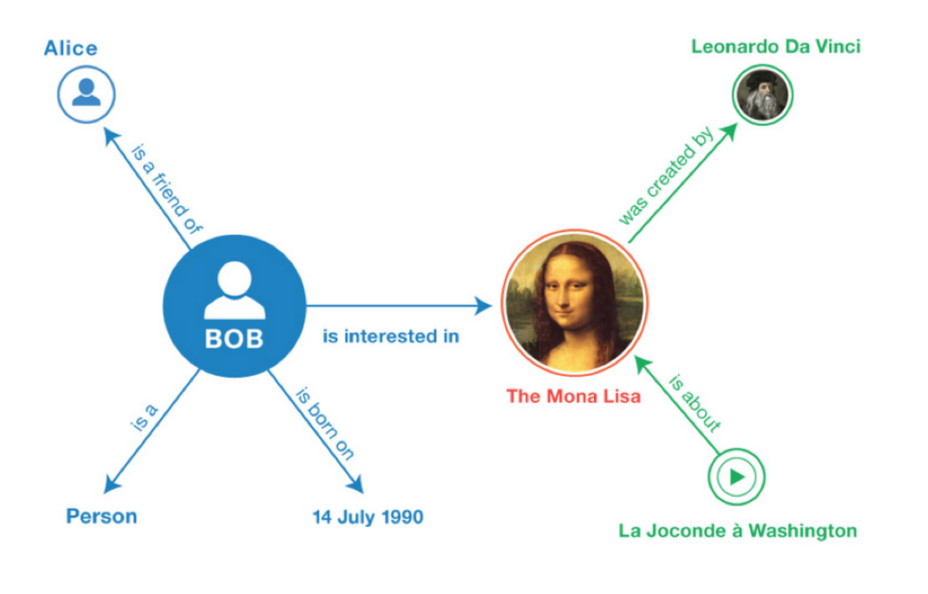
\includegraphics[width=\textwidth]{imagenes/capitulo3/grafoRDF}
		\caption{Grafo RDF}
	\end{subfigure}       
	\begin{subfigure}[h]{0.75\textwidth} 
		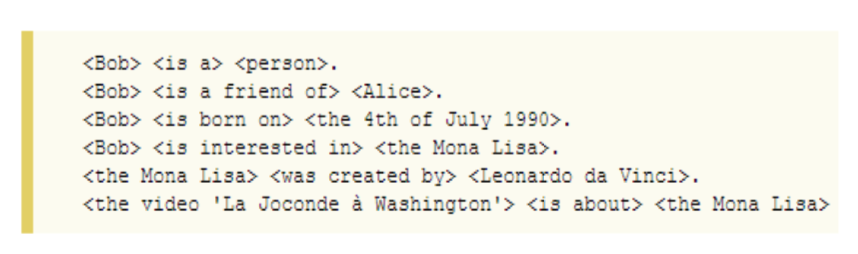
\includegraphics[width=\textwidth]{imagenes/capitulo3/ejemploRDF}
		\caption{Ejemplo RDF Tripleta}
	\end{subfigure}
	\caption{Ejemplo de grafo RDF \cite{aplicacion}}
	\label{fig:ejemploRDF}
\end{figure}

La estructura central del RDF es un conjunto de triples (tripletas), que se conoce como grafo RDF y que consta de tres componentes, en donde cada miembro puede ser una referencia a un símbolo (generalmente representado por un URI), que tiene un significado bien definido \cite{web-semantica-w3c}. La figura \ref{fig:tripleta} ilustra los tres componentes de un grafo RDF, y la figura \ref{fig:ejemploRDF} muestra un ejemplo.

\begin{enumerate}
	\item \textbf{Sujeto}: es el recurso, es decir, todo aquello que puede ser descrito.
	\item \textbf{Predicado}: introduce la propiedad que va a detallarse sobre el recurso.
	\item \textbf{Objeto}: es el valor de dicha propiedad.
\end{enumerate}

\begin{figure}[H]
	\centering
	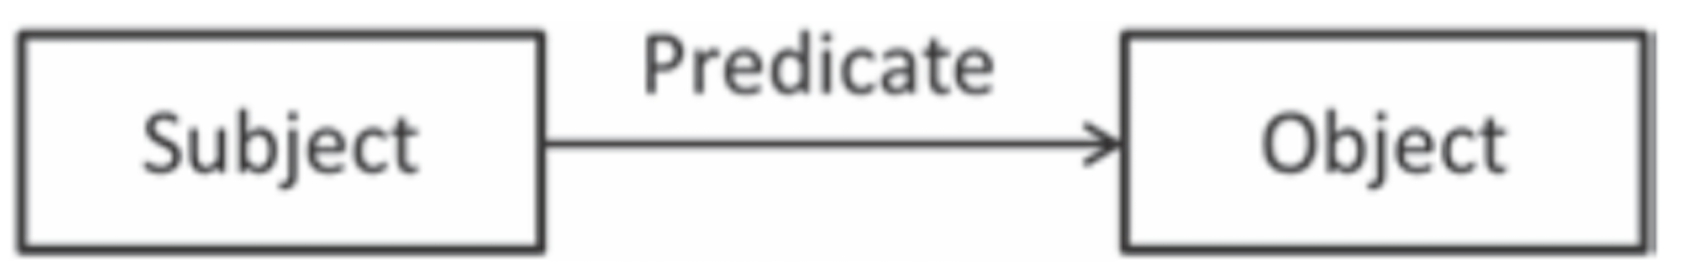
\includegraphics[width=0.48\linewidth]{imagenes/capitulo3/tripleta1}
	\caption{Estructura de un grafo RDF \cite{libro-gis}}
	\label{fig:tripleta}
\end{figure}



Básicamente RDF es un conjunto de declaraciones que definen clases y propiedades de los recursos. En la tabla \ref{tabla-rdf1} y \ref{tabla-rdf2} se muestra el vocabulario empleado por RDF \cite{tesis-otro}.


%en donde el sujeto y el objeto representan los dos recursos relacionados y el predicado representa la relación entre los dos recursos.


\begin{table}[H]
	\caption{Clases del vocabulario RDF}
	\label{tabla-rdf1}
		\centering
	\begin{tabular}{|
			>{\columncolor[HTML]{FFFFFF}}l |m{9cm}|}
		\hline
		\cellcolor[HTML]{EFEFEF}\textbf{CLASE} & \cellcolor[HTML]{EFEFEF} \textbf{DESCRIPCIÓN}\\ \hline
		\texttt{rdf:XMLLiteral}                         & La clase de los valores literales de los valores literales XML                         \\ \hline
		\texttt{rdf:Property}                         &  La clase de las propiedades RDF
		\\ \hline
		\texttt{rdf:Statement}                         &    La clase de las declaraciones RDF
		\\ \hline
		\texttt{rdf:Bag}                         &    La clase de los contenedores desordenados
		\\ \hline
		\texttt{rdf:Seq}                         &    La clase de los contenedores ordenados                      \\ \hline
		\texttt{rdf:Alt}                         &     La clase de los contenedores de alternativas                     \\ \hline
		\texttt{rdf:List}                         &  La clase de las listas RDF                        \\ \hline
	\end{tabular}
	
\end{table}

\begin{table}[H]
	\caption{Propiedades del vocabulario RDF}
	\label{tabla-rdf2}
		\centering
	\begin{tabular}{|
			>{\columncolor[HTML]{FFFFFF}}l |m{9cm}|}
		\hline
		\cellcolor[HTML]{EFEFEF}\textbf{PROPIEDAD} & \cellcolor[HTML]{EFEFEF} \textbf{DESCRIPCIÓN}\\ \hline
		\texttt{rdf:type}                         &      El sujeto es una instancia de una clase                    \\ \hline
		\texttt{rdf:first}                         &   El primer item en la lista RDF del sujeto                       \\ \hline
		\texttt{rdf:rest}                         &        El resto de la lista RDF del sujeto despúes del primer item                  \\ \hline
		\texttt{rdf:value}                         &    Propiedad idiomática usada para valores estructurados                       \\ \hline
		\texttt{rdf:subject}                         &     El sujeto de la declaración RDF del sujeto                     \\ \hline
		\texttt{rdf:predicate }                         &      El predicado de la declaración RDF del sujeto                    \\ \hline
		\texttt{rdf:object}                         &        El objeto de la declaración RDF del sujeto                  \\ \hline
	\end{tabular}
\end{table}

En la figura \ref{fig:ejemplo-rdf} podemos ver un ejemplo de RDF a partir del vocabulario que acabamos de ver en las tablas anteriores. Otro ejemplo puede verse en la figura \ref{fig:imagen1}, que muestra un conjunto de tripletas que indican la relación entre un recurso, nombre del recurso y geometría, es decir, en este caso el sujeto es el \textit{Recurso} que tiene la propiedad \textit{Nombre} cuyo valor es \textit{Quito}, además \textit{Recurso} tiene la propiedad \textit{Geometría} cuyo valor es \textit{Punto} y finalmente se indica que el sujeto \textit{Punto}, tiene la propiedad \textit{WKT} que indica el formato de la geometría, cuyo valor es \textit{POINT(-78.52495 -0.22985)} \cite{coursera}. 

\begin{figure}[H]
	\centering
	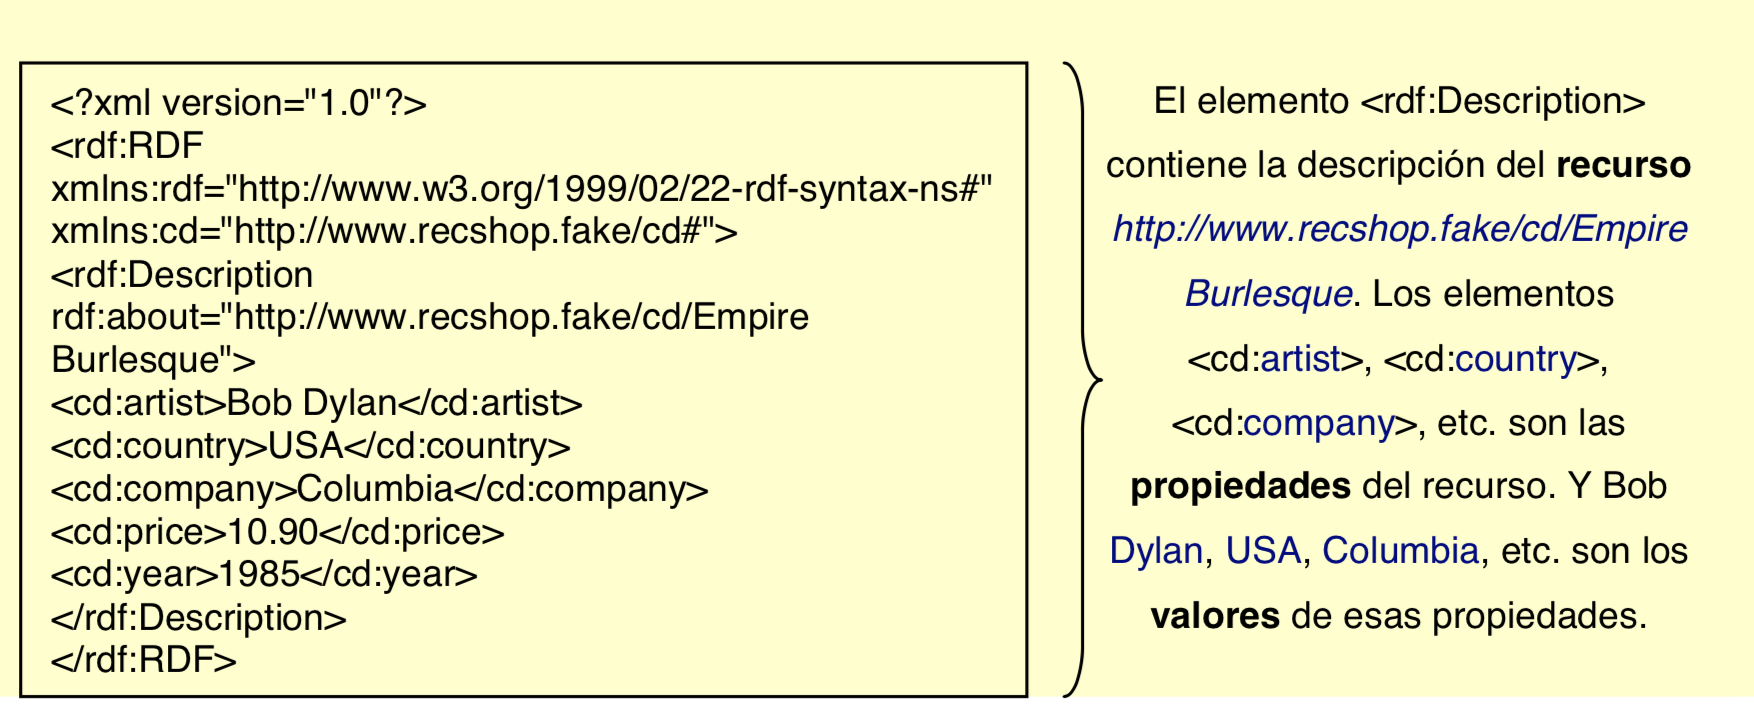
\includegraphics[width=0.9\linewidth]{imagenes/capitulo3/ejemplo-RDF}
	\caption{Descripción de un recurso musical en RDF \cite{web-semantica-w3c}}
	\label{fig:ejemplo-rdf}
\end{figure}

\begin{figure}[H]
	\centering
	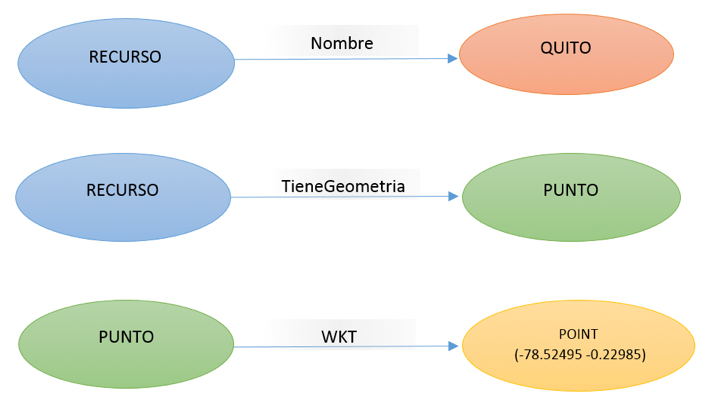
\includegraphics[width=0.73\linewidth]{imagenes/capitulo3/Imagen1}
	\caption{Ejemplo de tripletas \cite{coursera}}
	\label{fig:imagen1}
\end{figure}



Por tanto, se entiende que RDF es a la semántica lo que XML es a la sintaxis, ya que XML responde a la necesidad de representar sintácticamente el modelo planteado por RDF para archivos entendibles por ordenador \cite{web-semantica-w3c}.\\

Adicionalmente y sin entrar mucho en detalle, es necesario nombrar en esta capa el término \textbf{Linked Data}, el cual ha permitido introducir el concepto de ``Web de datos''. Linked Data es una área de investigación que estudia cómo hacer que los datos RDF estén disponibles en la Web e interconectarlos con otros datos con el objetivo de aumentar su valor para los usuarios. En resumen, es simplemente el uso de la Web para crear vínculos con tipo entre los datos de diferentes fuentes. Un ejemplo de ello es LinkedGeoData2, en donde los datos de OpenStreetMap están disponibles como RDF y se consultan utilizando el lenguaje de consulta declarativa SPARQL \cite{wkt-database, aplicacion}.\\

El siguiente diagrama (figura \ref{fig:lod-cloud-sm}) muestra los conjuntos de datos en la nube Linked Open Data así como sus relaciones en 2019. Cada nodo representa un conjunto de datos diferentes publicado en Linked Data y los arcos representan los enlaces RDF que existen entre los ítems de cada par de conjunto de datos relacionados. Como nota a la ilustración puede comentarse que el conjunto que aparece como nodo central es el perteneciente a DBpedia que es el referente a la abstracción semántica de la Wikipedia \cite{aplicacion}.

\begin{figure}[H]
	\centering
	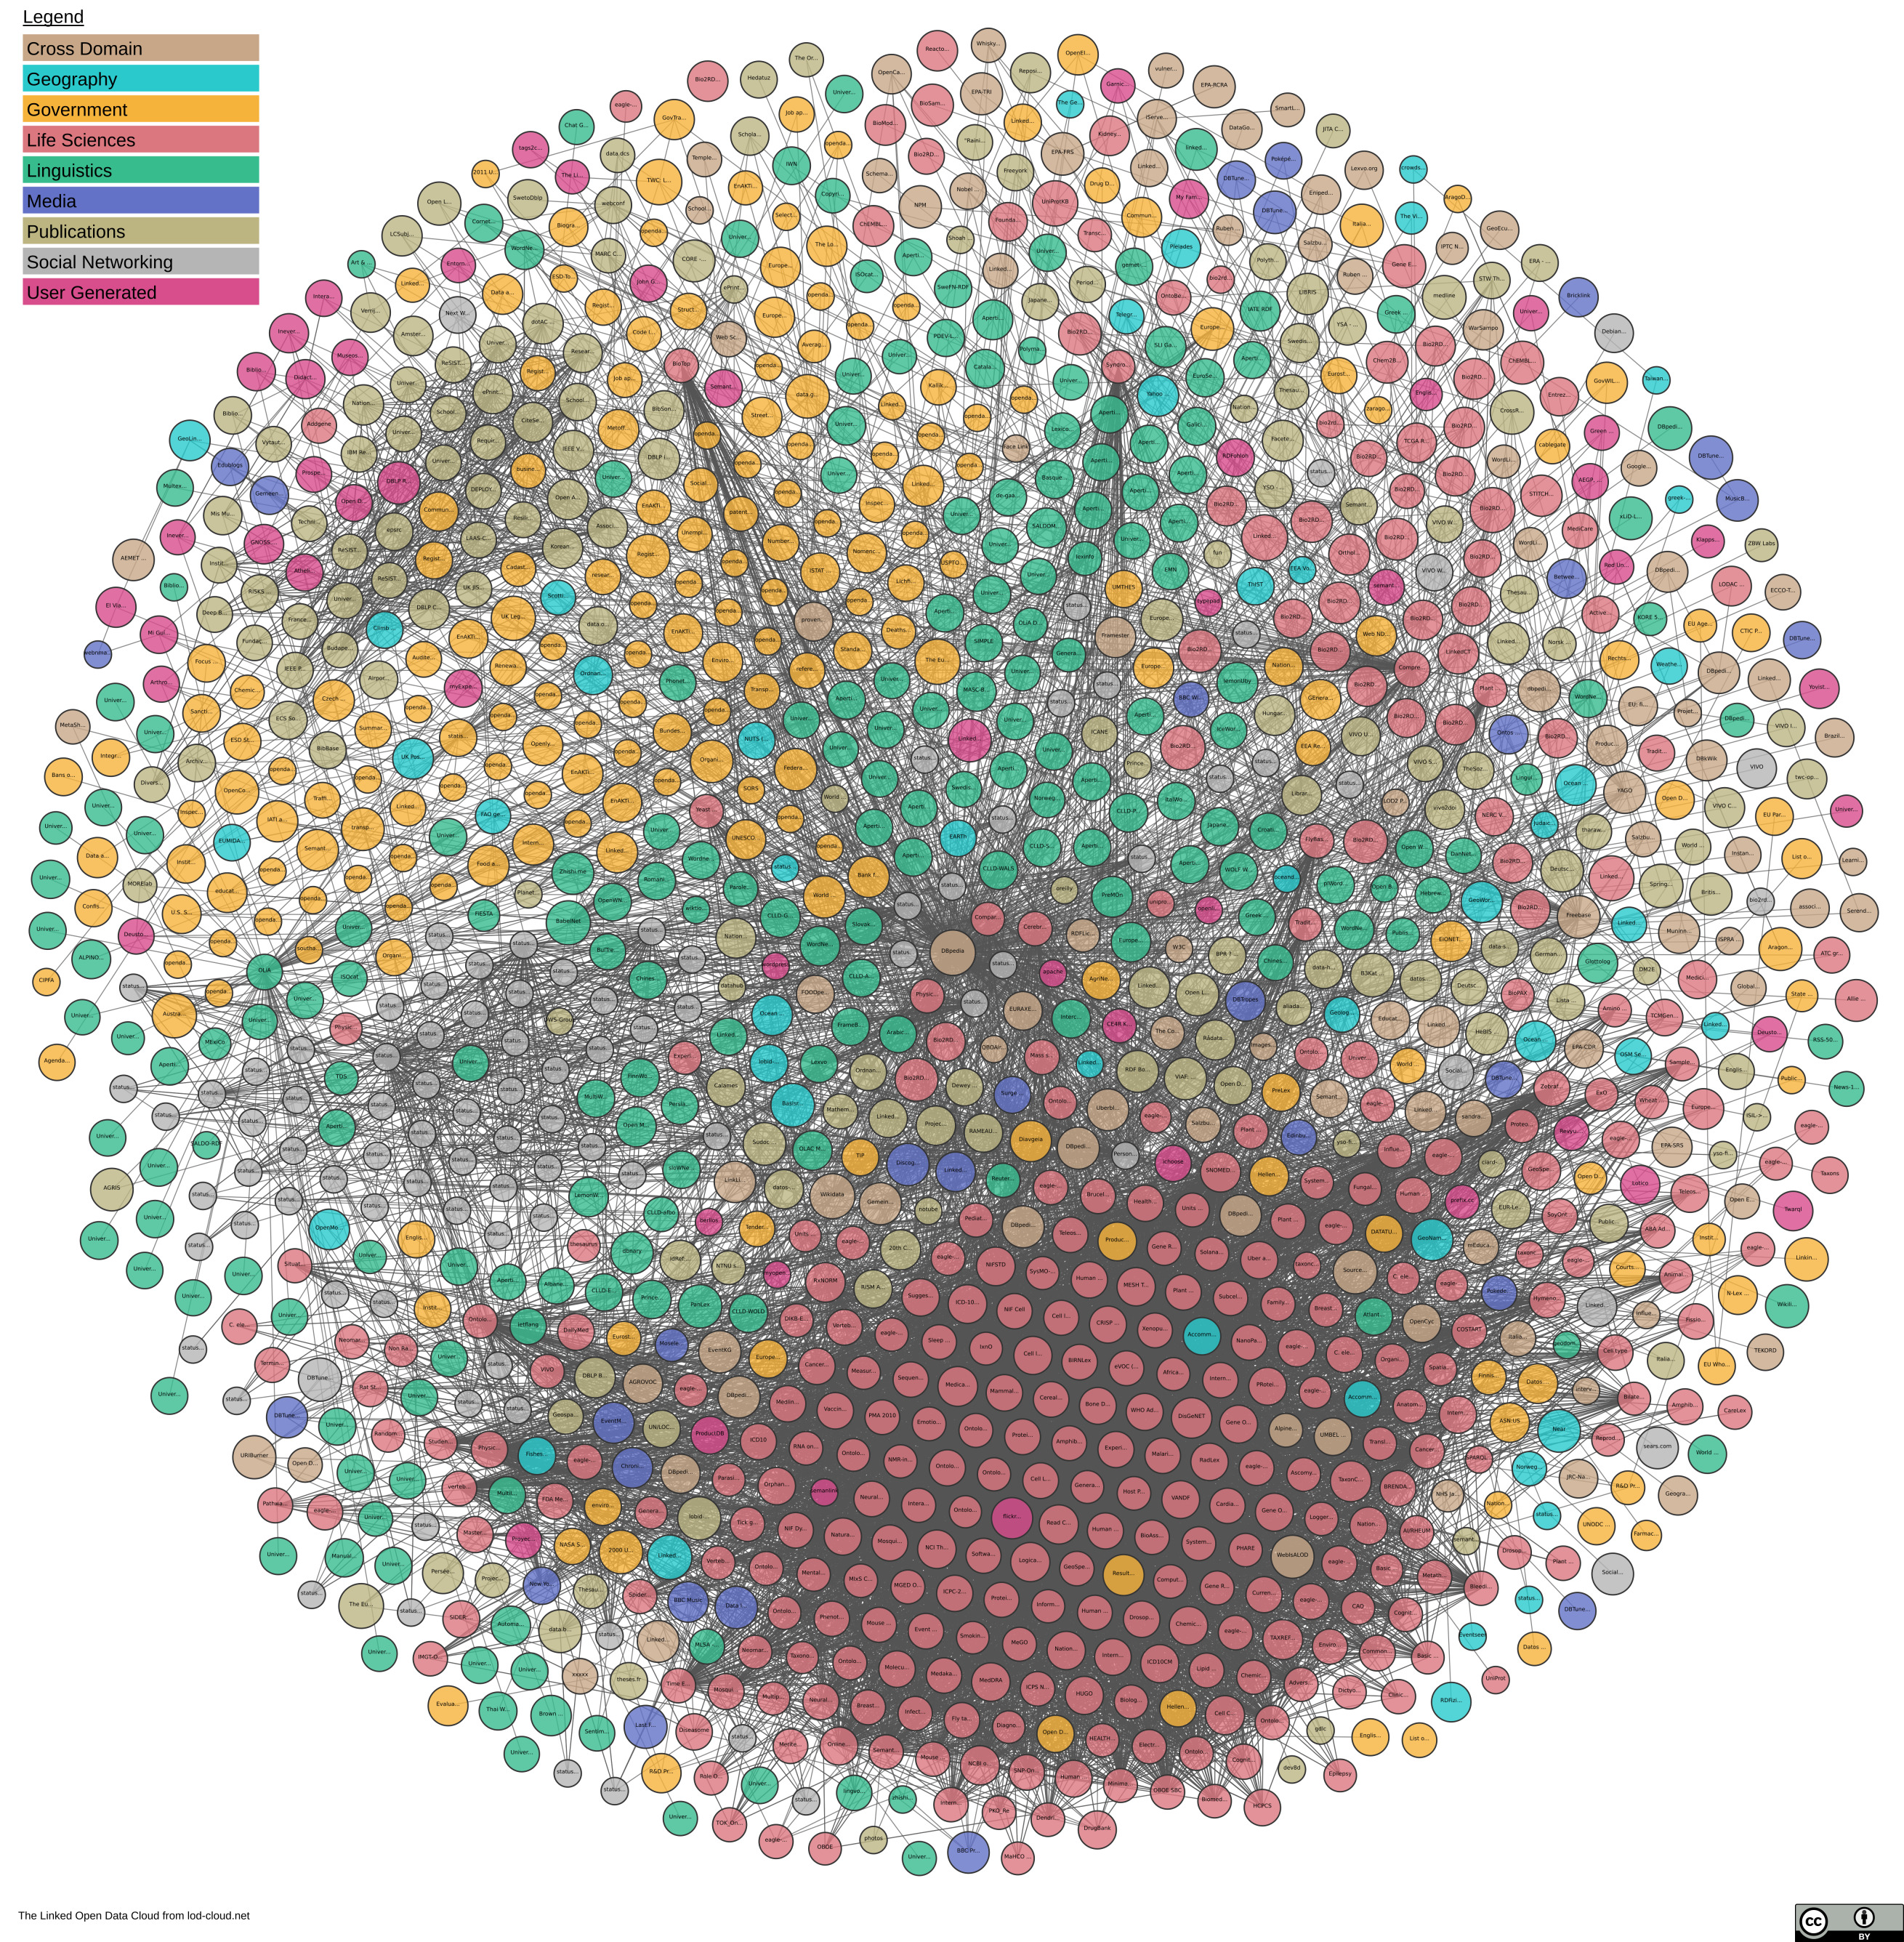
\includegraphics[width=0.9\linewidth]{imagenes/capitulo3/lod-cloud-sm}
	\caption{Diagrama Linked Open Data (\url{https://lod-cloud.net})}
	\label{fig:lod-cloud-sm}
\end{figure}





\subsection{Ontología} % Web Ontology Language (OWL)

% tesis
La \textbf{ontología} es un concepto filosófico adoptado por la Informática, que parte de la metafísica y que trata del ser en general y de sus propiedades trascendentales \cite{apuntes-clase-jose}. Se trata de un esquema conceptual que define los términos a utilizar para describir y representar un área de conocimiento dado, con el objetivo de facilitar la comunicación entre diferentes entidades, es decir, codifican el conocimiento de un dominio y de esta manera hacen el conocimiento reutilizable \cite{tesis}. Así, definen de forma estándar y consensuada un vocabulario de conceptos como las relaciones entre ellos dentro de un área concreta del conocimiento, formando redes jerárquicas semánticas y recogiendo reglas lógicas y restricciones para hacer comprender a las máquinas los conceptos de un determinado campo. Por ejemplo, \textit{una ontología de arte establece que todos los escultores son artistas pero no todos los artistas son escultores} \cite{web-semantica-w3c}. En una ontología nos podemos encontrar \cite{aplicacion, apuntes-clase-jose}:

\begin{figure}[H]
	\centering
	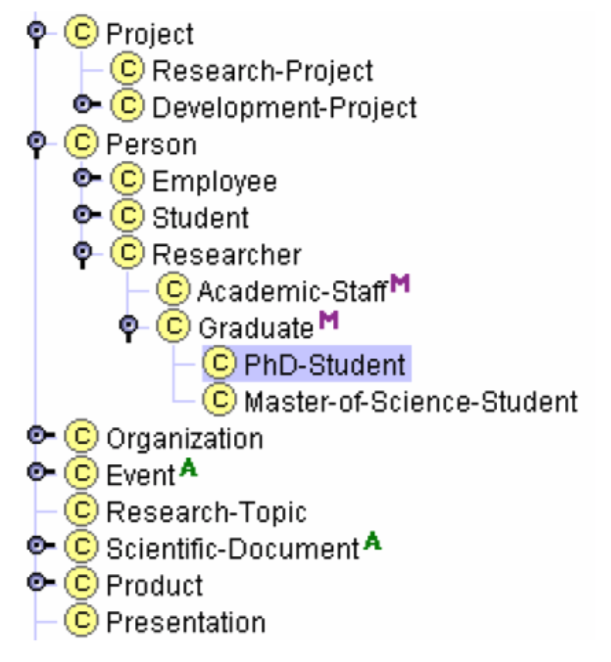
\includegraphics[width=0.55\linewidth]{imagenes/capitulo3/ejemplo-owl}
	\caption{Ejemplo de una ontología \cite{apuntes-clase-jose}}
	\label{fig:ejemplo-owl}
\end{figure}


\begin{itemize}
	\item \textbf{Conceptos}: sujetos básicos que se intentan formalizar sobre cualquier tipo de clase. En una ontología de deportes, cada clase sería un deporte: tenis, fútbol, baloncesto o natación.
	
	\item  \textbf{Relaciones}: enlace entre los conceptos, cómo interactúan los conceptos del dominio (subclase-de, parte-de).
	
	\item \textbf{Propiedades}: definen características o atributos de los conceptos.
	
	\item \textbf{Instancias}: objetos particulares de un concepto.
		
	\item \textbf{Funciones}: tipo de relación en la que el elemento es el resultado de la aplicación directa de una operación sobre varios conceptos de la ontología.
		
	\item \textbf{Axiomas}: teoremas que se declaran sobre las relaciones, y que deberán cumplir los elementos de la ontología. Es la clave de la inferencia de conocimiento. Por ejemplo, \textit{si A conoce B, B conoce A}.
	
	\item \textbf{Constantes}: permiten representar valores primitivos como cadenas de caracteres o valores numéricos
	
	\item \textbf{Restricciones}: descripciones sobre qué debe cumplirse para que un axioma sea cierto.
	
\end{itemize}

%Las ontologías pueden ser modeladas con diferentes técnicas de modelado de conocimiento y a su vez implementadas con diferentes lenguajes. Algunas de las técnicas de modelado son utilizando: marcos y lógica de primer orden, lógica descriptiva, UML o bien diagramas Entidad-Relación. Entre los lenguajes de implementación, el W3C recomienda RDF y OWL.

Una vez visto el concepto de ontología y su posible aplicación a la Web Semántica, es posible pasar a explicar RDF Schema y OWL.


\subsubsection{RDF Schema}

\textbf{Esquema RDF} o \textbf{RDFS} \textbf{(\textit{Resource Description Framework Schema})} es una extensión semántica que enriquece a RDF. Es un vocabulario que permite definir un primer sistema de jerarquías entre las clases de recursos, especificando las propiedades y relaciones admitidas entre ellas, es decir, permite a los usuarios definir características semánticas de los datos RDF y comprobar las restricciones semánticas \cite{web-semantica-w3c, libro-gis, aplicacion}. Igual que se han definido para RDF, existe un vocabulario empleado por RDFS (tablas \ref{tabla-rdfs1} y \ref{tabla-rdfs2}) \cite{tesis-otro}.



%Junto al RDF, se usa RDFS (RDF Schema) para definir las propiedades de los recursos y los tipos de recursos que son descritos. Es un mecanismo necesario para detallar cada elemento, especificar un vocabulario para definir las clases y propiedades, restringir las posibles combinaciones de clases y relaciones, y detectar violaciones de estas restricciones. Mientras un XML Schema puede ser utilizado para validar la sintaxis de un RDF/XML, un RDF Schema permite comprobar las restricciones semánticas.

\begin{table}[H]
	\caption{Clases del vocabulario RDFS}
	\label{tabla-rdfs1}
	\centering
	\begin{tabular}{|
			>{\columncolor[HTML]{FFFFFF}}l |m{8.9cm}|}
		\hline
		\cellcolor[HTML]{EFEFEF}\textbf{CLASE} & \cellcolor[HTML]{EFEFEF} \textbf{DESCRIPCIÓN}\\ \hline
		\texttt{rdfs:Resource}                         &        La clase de recurso, cada uno
		\\ \hline
		\texttt{rdfs:Literal}                         &        La clase del valor literal, por ejemplo, números enteros                  \\ \hline
		\texttt{rdfs:Class}                         &        La clase de las clases
		\\ \hline
		\texttt{rdfs:Datatype}                         &    La clase de los tipos de datos RDF                      \\ \hline
		\texttt{rdfs:Container}                         &   La clase de los contenedores RDF                       \\ \hline
	\end{tabular}
\end{table}

\begin{table}[H]
	\caption{Propiedades del vocabulario RDF}
	\label{tabla-rdfs2}
	\centering
	\begin{tabular}{|
			>{\columncolor[HTML]{FFFFFF}}l |m{8cm}|}
		\hline
		\cellcolor[HTML]{EFEFEF}\textbf{PROPIEDAD} & \cellcolor[HTML]{EFEFEF} \textbf{DESCRIPCIÓN}\\ \hline
		\texttt{rdfs:subClassOf}                         &         El sujeto es una subclase de una clase                 \\ \hline
		\texttt{rdfs:subPropertyOf}                         &     El sujeto es una subpropiedad de una propiedad                     \\ \hline
		\texttt{rdfs:domain}                         &           Un dominio de la propiedad del sujeto               \\ \hline
		\texttt{rdfs:range}                         &        Un rango de la propiedad del sujeto                  \\ \hline
		\texttt{rdfs:label}                         &        Un nombre para el sujeto legible por personas                   \\ \hline
		\texttt{rdfs:comment}                         &        Una descripción del recurso sujeto                  \\ \hline
		\texttt{rdfs:member}                         &        Un miembro del recurso sujeto                  \\ \hline
		\texttt{rdfs:seeAlso}                         &              Más información sobre el recurso sujeto            \\ \hline
		\texttt{rdfs:isDefinedBy}                         &       La definición del recurso sujeto. 
		\\ \hline
	\end{tabular}
\end{table}

Sin embargo, RDFS tiene limitaciones al carecer de expresividad para: información negativa (las mujeres no son hombres), cuantificadores (para que alguien sea considerado madre debe tener al menos un hijo), cardinalidad (un buen estudiante tiene que tener aprobadas más de 4 asignaturas) y no permite atributos de propiedades (transitiva, simétrica, inversa). Por todo esto y más, no se considera lo bastante completo para describir los recursos de la Web con el detalle necesario, pero se utiliza porque se puede emplear en muchos dominios y actuar de puente entre vocabularios \cite{aplicacion}.

\subsubsection{OWL}

\textbf{OWL} \textbf{(\textit{Ontology Language Web})} es un lenguaje ontológico para la Web Semántica con significado formalmente definido, sirve para definir ontologías Web estructuradas y provee de más vocabulario para la descripción de propiedades y clases, por ejemplo: relaciones entre clases, cardinalidad, equivalencia y características de propiedades (figura \ref{fig:ejemplo-owl}). Realmente, OWL es una extensión del lenguaje RDF y emplea tripletas de RDF (figura \ref{fig:nomenclatura}), aunque es un lenguaje con más poder expresivo \cite{aplicacion}.

\begin{figure}[H]
	\centering
	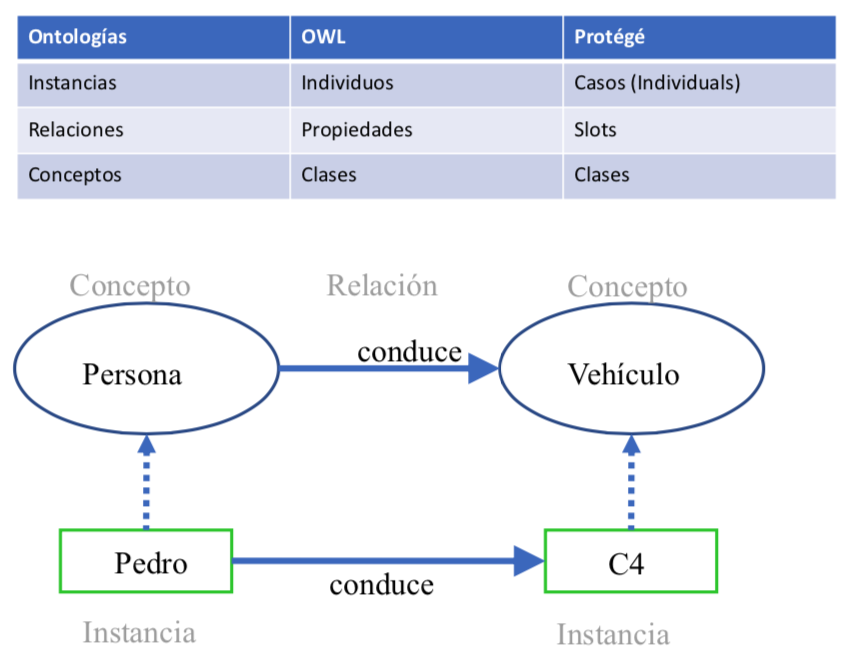
\includegraphics[width=0.67\linewidth]{imagenes/capitulo3/nomenclatura}
	\caption{Nomenclatura básica ontología OWL \cite{apuntes-clase-jose}}
	\label{fig:nomenclatura}
\end{figure}


%OWL puede formularse en RDF, que ofrece la base adecuada para desarrollar ontologías, y mejora la capacidad expresiva de RDFS. Al construirse sobre RDF, las ontologías OWL podrán ser distribuidas en diferentes sistemas y ser compatibles con otros estándares web.\\
En Octubre de 2009 nació \textit{OWL 2 Web Ontology Language} como recomendación del W3C para la edición de ontologías, extensión de la primera versión OWL 1 publicada en 2004. OWL 1 proporciona tres lenguajes, cada uno con nivel de expresividad mayor que el anterior, diseñados para ser usados por comunidades específicas de desarrolladores y usuarios \cite{owl-tipos}. En OWL 2 se definen tres nuevos perfiles y se proporcionan tres sublenguajes que ofrecen ventajas en escenarios particulares, todos más restrictivos que OWL DL y cada uno con diferentes aspectos expresivos a cambio de diferentes beneficios computacionales y/o de implementación \cite{aplicacion}. 

\begin{itemize}
	\item \textbf{OWL Lite}: diseñado para aquellos usuarios que necesitan principalmente creación de jerarquías y restricciones simples.
	
	\item \textbf{OWL DL}: es el lenguaje habitual de ontologías diseñado para aquellos usuarios que quieren la máxima expresividad conservando completitud computacional, es decir, está basado en lógica descriptiva y proporciona la máxima capacidad de expresión para garantizar computabilidad y decidibilidad (todas las conclusiones pueden ser deducidas y todos los cálculos se realizan en un tiempo finito).
	
	\item \textbf{OWL Full}: diseñado para aquellos usuarios que quieren máxima expresividad y libertad sintáctica de RDF sin garantías computacionales, es decir, permite expresividad de segundo orden, pero sin decidibilidad (no hay garantía computacional).
\end{itemize}



Por otro lado, las ontologías deben de cumplir unas características: sintaxis bien definida, semántica específica, expresividad, fácilmente traducible entre los lenguajes ontológicos y eficiencia para realizar razonamientos \cite{apuntes-clase-jose}.\\

No obstante, escribir en lenguajes como RDF y OWL resultan sumamente difícil y propensos a errores. Afortunadamente, existen en el mercado entornos gráficos para visualizar y construir ontologías de forma más sencilla, como \textbf{Protegé}, software desarrollado por la Universidad de Stanford que permite editar ontologías con una interfaz simple y en un entorno de menús, botones, cuadros de diálogo o representaciones gráficas fáciles de usar, tan importantes para una tarea con tanta de abstracción y síntesis.

\subsection{Lenguajes de consulta}


Por último, nos queda presentar el lenguaje de consulta semántica SPARQL, estándar ampliamente utilizado para consultar datos RDF. Además de SPARQL se dispone de GeoSPARQL, extensión de SPARQL que admite operaciones geoespaciales, y que será introducido en el capítulo siguiente.


\subsubsection{SPARQL}

% dbpedia, que es la representación en RDF en wikipedia la dbpedia en español


% COURSERA: La Web Semántica: Herramientas para la publicación y extracción efectiva de información en la Web
%Hola, bienvenido a nuestro curso sobre la web semántica, en este video comenzaremos a ver algunas de la nociones básicas sobre el lenguaje de consulta SPARQL, en particular veremos la nociones de variables y patrones en SPARQL. Como ya hemos mencionado en los videos anteriores en la web existe una multitud de base de datos de RDF, por ejemplo dbpedia, que es la representación en RDF en wikipedia la dbpedia en español y IMDB que es una base de películas, etcétera. Muchas de estas bases RDF permiten acceder a sus datos utilizando el lenguaje de consulta SPARQL, recuerde que SPARQL es un lenguaje que nos permite escribir de manera precisa la información que queremos extraer y que es procesable por un computador, vale decir un computador puede de manera automática construir las respuestas de una consulta SPARQL. Entonces en esta base de datos RDF nos permiten utilizar este lenguaje SPARQL y la forma de hacerlo es a través de lo que es llamado un SPARQL endpoint, que es un servicio web donde uno puede colocar este tipos de consultas. En esta transparencia puede ver la dirección de dos de estos servicios web, la primera de ellas es el SPARQL endpoint de dbpedia que es dbpedia.org/sparql, la segunda es el SPARQL endpoint de dbpedia en español.

%En esta transparencia usted puede ver este grafo RDF escrito en un archivo como una secuencia de triples, recuerde cuando teníamos una secuencia de triples en primer lugar especificamos los prefijos que vamos a utilizar en los URIs, recuerden que estos prefijos son utilizados para simplificar la notación que tenemos en estos URIs Una vez que hemos escrito estos prefijos en este caso tenemos dbpprop, dbpedia-owl y dbpedia construimos nuestros triples en esta caso tenemos cuatro triples el primero de ellos es dbpedia:Santiago rdf:type y dbpedia-owl:place, en este triple estamos diciendo que Santiago es de tipo lugar. En esta transparencia usted puede ver un grafo en la dbpedia con datos sobre lugares, esto simplemente es parte del grafo anterior donde decíamos bueno dbpedia:Santiago es de tipo lugar, que se encuentra en Chile y que su nombre oficial es Santiago. En esta transparencia usted tambien puede ver una consulta SPARQL y a continuación mostraremos las distintas partes de esta consulta, en primer lugar tenemos el encabezado de la consulta que puede ver en amarillo, este encabezado se puede distinguir a través de la palabra SELECT. En segundo lugar tenemos el patrón de la consulta que en este caso también esta desatascado en amarillo y que se encuentra dentro de la cláusula where. Es importante destacar que el patrón sigue la estructura sujeto, predicado, objeto. Por ejemplo en este caso tenemos un patrón de nuevo podemos ver este patrón en amarillo en el cual tenemos dos triples, en el primer triple ?X dbpprop:officialName ?name tenemos como sujeto a X, como predicado a dbprop:officialName y como objeto a name. En el segundo triple tenemos como sujeto a X, como predicado a rdf:type y como objeto a dbpedia-owl:Place. También es importante destacar que en este patrón tenemos variables y tenemos URIs, cada variable en una consulta SPARQL comienza con el signo de pregunta. En este caso entonces, tenemos como variables a signo de pregunta X y signo de pregunta name. También en una consulta SPARQL podemos tener URIs y en estos URIs utilizamos la notación usual, por ejemplo en esta consulta tenemos el URI dbpprop:officialName, en este caso estamos usando el prefijo dbpprop: ¿Cómo se calcula la respuesta a una consulta SPARQL? Bueno, en el patrón remplazamos cada variable por un URI o por un literal, y lo que es importante es que los triples resultantes de este remplazo debe estar en el grafo RDF. por ejemplo, en este caso podemos remplazar como he mostrado en la figura la variable X por dbpedia:Santiago y la variable name por Santiago. Si hacemos este remplazo entonces en el primer triple vamos a obtener el triple de dbpedia:Santiago, dbpprop:officialName Santiago que es un type que esta en el grafo RDF como es marcado en rojo. Lo que es importante en este caso es que tenemos que hacer el mismo remplazo en el segundo triple, y en este caso vamos a obtener el triple dbpedia:Santiago rdf:type, dbpedia-owl:place que tambien esta en nuestro grafo RDF. Por lo tanto en este caso tenemos un remplazo exitoso. ¿Para qué sirve el encabezado de una consulta SPARQL? El encabezado nos indica en este caso tenemos SELECT ?name por lo tanto nos está indicando que vamos a retornar los valores que hemos dado a la variable name, en este caso Santiago vale decir, esta consulta nos permite encontrar todos los nombres oficiales de los lugares que tenemos en dbpedia.

\textbf{SPARQL} es un lenguaje estandarizado por la W3C para el desarrollo de la Web Semántica y que permite escribir de manera precisa la información que queremos extraer, es decir, es una especificación que ofrece un lenguaje y protocolos para consultar y manipular RDF \cite{tesis-otro}. En la figura \ref{fig:sparql}, podemos encontrar una consulta básica de selección SPARQL y comprobar que la estructura de este lenguaje se asemeja a SQL. Entre las características de SPARQL, resaltan: 

\begin{itemize}
	\item Lenguaje de consulta.
	\item Formato XML, JSON, CSV y TSV  para resultados en una consulta.
	\item Actualización de grafos RDF.
	\item Protocolo para RDF.
	\item Descubrir información acerca de la información  almacenada (\textit{dataset}).
	\item Manejo de grafos mediante el protocolo HTTP.
\end{itemize}

%\begin{table}[H]
%	\caption{Características de SPARQL}
%	\label{carac-sparql}
%	\centering
%	\begin{tabular}{|l|}
%		\hline
%		  Lenguaje de consulta \\ \hline
%		 Formato XML, JSON, CSV y TSV  para resultados en una consulta \\ \hline
%Actualización de grafos RDF	\\ \hline
%	Protocolo para RDF	\\ \hline
%	Descubrir información acerca de la información  almacenada (\textit{dataset})	\\ \hline
%	 Manejo de grafos mediante el protocolo HTTP 	\\ \hline
%	\end{tabular}
%\end{table}

\begin{figure}[H]
	\centering
	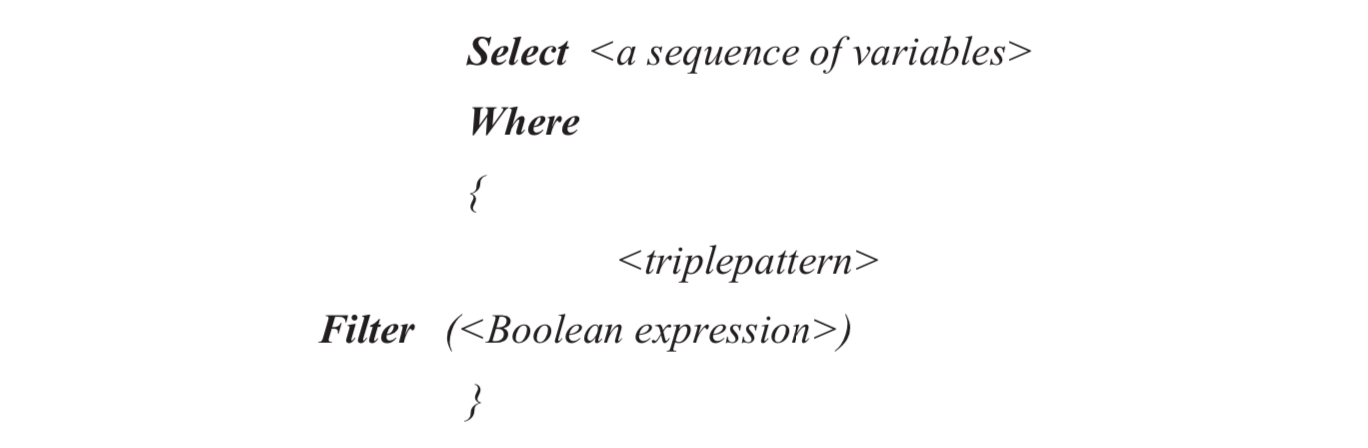
\includegraphics[width=1.1\linewidth]{imagenes/capitulo3/sparql}
	\caption{Estructura de una consulta en SPARQL}
	\label{fig:sparql}
\end{figure}

Los resultados de una consulta están restringidos por una sección \texttt{WHERE}, que proporciona el patrón de gráfico básico para que coincida con el gráfico de datos. El patrón gráfico consiste en un conjunto de triples, que forman un gráfico, donde un elemento de un triple puede ser un URI de un recurso, un valor de datos (en el caso del objeto triple) o una variable. Una variable tiene el prefijo con el signo de interrogación y puede aparecer en la sección \texttt{SELECT} (la variable de salida). La sección \texttt{WHERE} también puede contener cláusulas \texttt{FILTER}, que filtran por ejemplo, cadenas y valores numéricos usando varias funciones (predicados) \cite{tesis-otro}.\\

Un ejemplo simple de una consulta SELECT se encuentra en la figura \ref{fig:ejemplo-sparql}, en donde se quieren obtener de la Dbpedia, los ingenieros que residen en ciudades con una población de más de 10000000 habitantes. En la figura \ref{fig:salida-sparql} se puede observar la salida a dicha consulta \cite{tesis-otro}.

\begin{figure}[H]
	\centering
	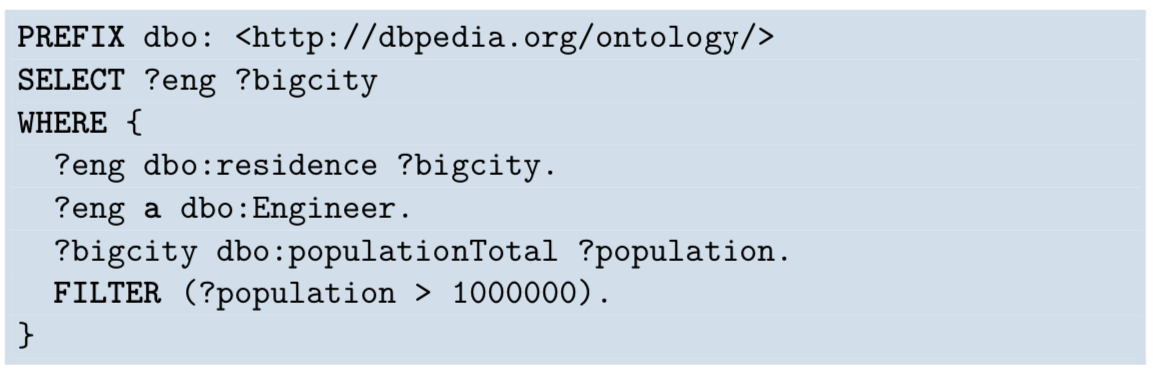
\includegraphics[width=0.9\linewidth]{imagenes/capitulo3/consulta}
	\caption{Ejemplo de consulta de SPARQL \cite{tesis-otro}}
	\label{fig:ejemplo-sparql}
\end{figure}

\begin{figure}[H]
	\centering
	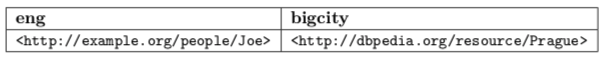
\includegraphics[width=0.9\linewidth]{imagenes/capitulo3/salida-sparql}
	\caption{Respuesta a la salida de la consulta de la figura \ref{fig:ejemplo-sparql}}
	\label{fig:salida-sparql}
\end{figure}


%En la figura 2.3 se muestra un ejemplo de consulta SPARQL, haciendo referencia a las tripletas de la figura 2.2, se observa la estructura de la consulta para obtener los datos deseados como el Nombre del recurso, tipo de geometría y la geometría en formato WKT. Lo que se encuentra en el recuadro de color verde permite identificar el recurso, en este caso “Quito”, posteriormente en el recuadro de color rojo se observa la parte de la consulta que permite obtener el tipo de geometría del recurso “Quito” y finalmente en el recuadro de color azul se encuentra la parte de la consulta que permite obtener la geometría en formato WKT del recurso “Quito”, tambíen se muestra el resultado generado por la consulta SPARQL. 

Como hemos comentado anteriormente, la herramienta Protegé nos permite construir contologías de manera más sencilla y rápida, sin embargo, también ofrece herramientas para realizar consultas con SPARQL. No obstante, aunque SPARQL sea un lenguaje ampliamente utilizado para consultar ontologías RDF, carece de las construcciones necesarias para consultar datos espaciales. Por lo que haremos uso del lenguaje GeoSPARLQ, introducido en el siguiente capítulo. \\

 Con esto hemos terminado de explicar las tecnologías de la Web Semántica. En la figura \ref{fig:arquitectura2copia} podemos apreciar el recorrido que hemos hecho por las distintas capas que tiene la arquitectura para la Web Semántica. Como el resto de capas no resultan relevantes para nuestro proyecto, se ha obtado por no exponerlas, para así enfocar el presente trabajo en el objetivo planteado al principio del mismo. En suma, el objetivo de la Web Semántica es que la Web pase de ser una colección de documentos a convertirse en una base de conocimiento (figura \ref{fig:mapawebsemantica-3}).

\begin{figure}[H]
	\centering
	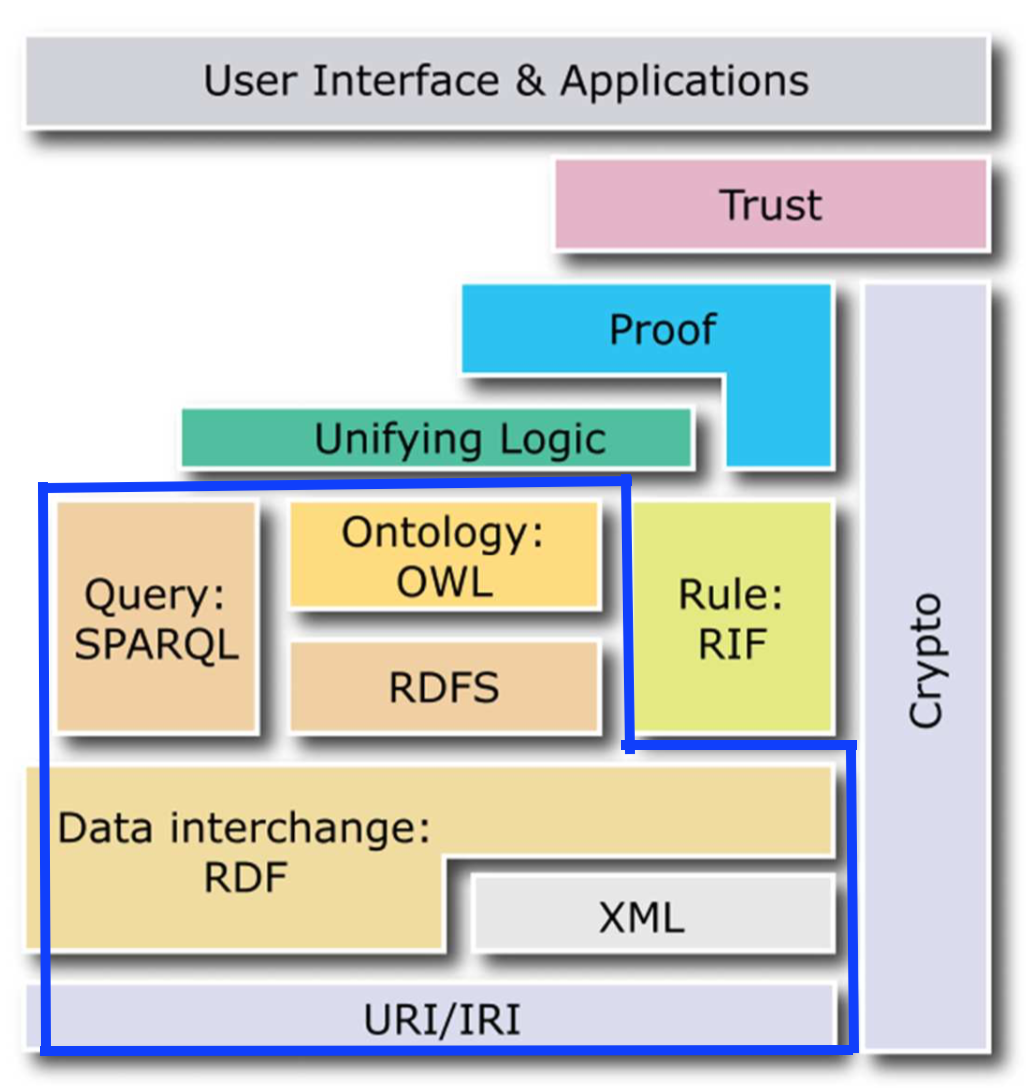
\includegraphics[width=0.52\linewidth]{imagenes/capitulo3/arquitectura2copia}
	\caption{Tecnologías de la Web Semántica explicadas \cite{apuntes-clase-jose}}
	\label{fig:arquitectura2copia}
\end{figure}

En otro orden de ideas y haciendo referencia a las capas de la Web Semántica que acabamos de comentar, \textit{¿de qué herramientas disponemos para manejar las tecnologías que acabamos de exponer?} En el mercado, nos podemos encontrar diversas herramientas de la Web Semántica. De entre todas las posibles, nosotros nos vamos a centrar en dos: 

\begin{enumerate}
	\item \textbf{Protegé}: editor libre y marco de ontología de código abierto para construir un sistema de adquisición de conocimiento, apoyado por una fuerte comunidad académica \cite{protege}. 
	
	\item \textbf{GraphDB}: familia de bases de datos RDF altamente eficientes, robustas y escalables. Este software agiliza la carga y el uso de conjuntos de datos en la nube de datos vinculados, así como sus propios recursos \cite{graphdb}.
\end{enumerate}

 Como primera opción se consideró usar solo Protegé, pero debido a diversos problemas que comentaremos más adelante, se buscó una alternativa, en este caso, GraphDB.  


\begin{figure}[H]
	\centering
	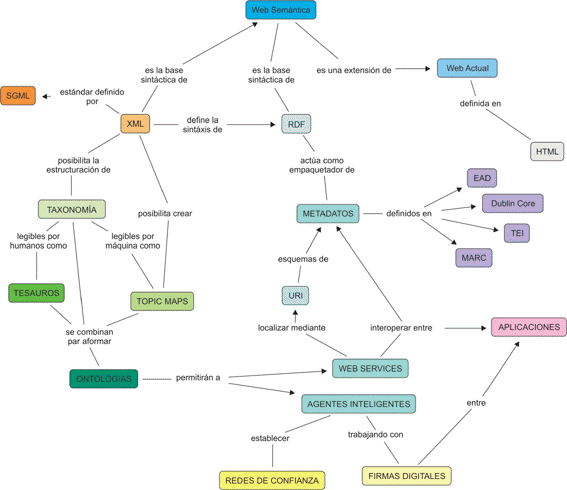
\includegraphics[width=1\linewidth]{imagenes/capitulo3/mapawebsemantica-3}
	\caption{Mapa conceptual de la Web Semántica \cite{imagen-final-esquema-ws}}
	\label{fig:mapawebsemantica-3}
\end{figure}




\section{¿Qué no es la Web Semántica?}

Una vez expuestos los contenidos que comprenden la Web Semántica, es necesario enfatizar qué no es la Web Semántica, con el objeto de evitar posibles confusiones futuras. Durante el presente trabajo, hemos hablado de que la Web Semántica es una extensión de la actual Web, por tanto diremos que una Web no es Semántica cuando sea diferente a la actual Web y tenga estándares incompatibles con la Web actual \cite{introduccion}. Además, debe seguir cumpliendo las características que conforman la Web, puesto que una Web de navegacioón compleja no transparente y difícil de usar para usuarios, tampoco entraría dentro de lo que llamamos Web Semántica. Además, no todos los navegadores hacen uso de búsquedas semánticas, ya que la mayoría se basan por similtudes con las palabras usadas para la búsqueda sin hacer uso de la interpretación de la información.\\

Adicionalmente, la evolución de la Web 2.0 conocida como Web 3.0, es confundida erróneamente con la Web Semántica, pero con la que no tiene nada que ver. Puesto que la Web 3.0 es lo que se experimenta en el dispositivo móvil cuando, por ejemplo, se abre la aplicación de Twitter y se consulta la información de la red social sin necesidad de abrir el navegador \cite{web-nueva}.

\section{Aplicaciones de la Web Semántica}


%Prototipo de un sistema semántico de diagnosis para congestiones de tráfico en carretera desarrollado por IBM (68), donde se presenta un prototipo que analiza de forma semántica y mediante enfoques de inteligencia artificial el histórico de congestiones de trafico para determinar las causas de situaciones inesperadas en casi tiempo real de la situación del trafico en la ciudad de Dublín.
%
%
%Aplicación de la Web Semántica en Trafico
%
%
%Reino Unido (data.gov.uk)
%
%El principal ejemplo encontrado con información de tráfico es el proporcionado desde el apartado transporte de la iniciativa de datos gubernamentales del Reino Unido (58), que permite consultar la información sobre estaciones de tren, aeropuertos y paradas de autobús entre otros, mediante consultas SPARQL.
%Por ejemplo para las estaciones de tren, se pueden lanzar las consultas mediante una interfaz similar a la de la ilustración, obteniendo el listado de las estaciones resultantes en diferentes formatos disponibles (ilustración 19):
%
%Desde data.gob.uk, también se puede acceder a información como los datos de tráfico, eventos planeados y no planeados en (59) pero esta vez en formato XML, siguiendo la estructura propuesta por DATEX II v1.0. El ejemplo de futuros eventos planificados puede consultarse en (60).
%Otra información disponible son los datos relativos a los conteos de tráfico en una región, pero estos sólo están disponibles en CSV o bien en PDF, sin integrar tampoco formatos RDF. Se pueden consultar desde (61).
%
%Estos ejemplos, son interesantes debido al tipo de información que publican, pero es necesario destacar que no se utilizan estándares de Web Semántica en la publicación de los datos, con lo que no se alcanzarían las 4 estrellas de la escala comentada en el apartado 4.2 Linked Data.

%Directorios y catálogos de documentos.
%Openguides.org
%www.dmoz.org
%Redes Sociales. FOAF
%http://www.foaf-project.org/
%Buscadores semánticos.
%http://www.aktors.org/technologies/csaktivespace/

%Buscadores Semánticos: Satisfacer las expectativas de búsqueda de usuarios que requieren resultados precisos.

% http://www.fgcsic.es/lychnos/es_es/articulos/construyendo_una_web_semantica

Los conceptos que acabamos de ver han repercutido en la actualidad, ya que existen diversas aplicaciones que de una forma u otra se basan en tecnologías semánticas para la Web. A continuación, mostramos algunas \cite{cwb}:

\begin{itemize}
	\item % http://www.fgcsic.es/lychnos/es_es/articulos/construyendo_una_web_semantica
	\textbf{Producción científica}: en el campo de la ciencia, la publicación de resultados de la experimentación es fundamental para la comunidad científica. Un ejemplo de ello es el portal \textbf{GoPubMed}\footnote{Actualmente no disponible (\url{https://www.gopubmed.org/})}, que ofrece un buscador semántico de publicaciones científicas en el área de la biomedicina, a través de la ontología \textit{Gene Ontology} que unifica y estructura la terminología sobre genes y productos génicos de un amplio número de organismos. Permite localizar textos relevantes no sólo por la ocurrencia de determinadas palabras clave sino por la relación semántica existente entre conceptos biomédicos. 
 
	% http://www.fgcsic.es/lychnos/es_es/articulos/construyendo_una_web_semantica
	%La publicación no solo de los resultados de una investigación sino también de los datos experimentales sobre los que se ha basado permitirá una mayor colaboración y transparencia en el ámbito de la investigación científica. Proyectos financiados por la Unión Europea, como OpenKnowledge o LiquidPub, han investigado formas novedosas de colaboración y publicación distribuida en la Web que apuntan a que vamos a ser testigos de un cambio importante en cómo se publican, se comparten y se diseminan los resultados científicos.
	
	%\item % http://www.fgcsic.es/lychnos/es_es/articulos/construyendo_una_web_semantica
	%\textbf{Gobiernos abiertos}: Numerosos gobiernos nacionales están impulsando iniciativas de «gobierno abierto», haciendo públicos los conjuntos de datos en su posesión para promover la transparencia, aumentar la eficiencia administrativa y estimular el crecimiento económico. La combinación de estos datos mediante mashups –aplicaciones web que combinan datos y funcionalidades de diferentes fuentes– permite realizar consultas y presentar sus resultados de forma novedosa y creativa. En 2009, en una localidad del estado de Ohio, en Estados Unidos, un abogado creó un mashup que combinaba los datos públicos sobre la ubicación de las tuberías de agua corriente con los datos obtenidos del censo municipal sobre qué viviendas estaban habitadas por familias afroamericanas. El mapa resultante reveló que, en determinados barrios limítrofes, el ayuntamiento claramente discriminaba a los hogares afroamericanos. En consecuencia, un juez decretó una indemnización por daños y perjuicios.
	
	% hablar sobre la página esa que tiene Londres - London Data store
	\item \textbf{Gobiernos abiertos}: muchos gobiernos han impulsando iniciativas de \textit{gobierno abierto}, con el fin de hacer públicos conjuntos de datos para ayudar a comprender la ciudad y desarrollar soluciones a los problemas. \textbf{London Datastore} (\url{https://data.london.gov.uk}) es un portal gratuito y abierto para compartir datos donde cualquiera puede acceder a datos relacionados con Londres. Por ejemplo, en el apartado \textit{transporte} de esta iniciativa de datos gubernamentales del Reino Unido, nos permite consultar la información sobre estaciones de tren, aeropuertos y paradas de autobús entre otros, mediante consultas SPARQL.

	% http://www.fgcsic.es/lychnos/es_es/articulos/construyendo_una_web_semantica
	\item \textbf{Colaboración popular masiva}: la exposición, edición, compartición e interconexión de datos estructurados en la Web es muy común. \textbf{LinkedGeoData} es una iniciativa para añadir una dimensión espacial a los datos publicados en la Web Semántica y se basa en la información recogida por el proyecto \textit{OpenStreetMap}\footnote{Mapa mundial abierto al que cualquiera puede añadir datos, parecido al funcionamiento de Wikipedia.}. Un ejemplo de ello, fue cuando a finales del 2009 muy pocas áreas de la ciudad de Port-au-Prince en Haití estaban etiquetadas. Pero justo después del terremoto de enero de 2010, cuando se hicieron públicas imágenes de satélite del país, miles de personas estudiaron estas imágenes y comenzaron a anotar en el \textit{OpenStreetMap} información detallada sobre las zonas devastadas: carreteras bloqueadas, edificios dañados, hospitales de campaña o muelles en los que atracaban los barcos con ayuda humanitaria. Todos estos datos fueron de gran utilidad para los equipos de rescate que sobre el terreno que consultaban esta información con sus dispositivos móviles.
	
\end{itemize}


%\section{Retos del futuro}

% http://www.fgcsic.es/lychnos/es_es/articulos/construyendo_una_web_semantica
%La web de datos, con sus vocabularios y ontologías, es un ente abierto y dinámico. Continuamente aparecen nuevos datos y nuevos enlaces entre ellos, mientras otros quedan obsoletos y se eliminan. Además, los servidores que hospedan estos datos a veces no están activos, bien porque han caído o bien porque están bajo mantenimiento. Eso implica una gran variabilidad semántica en los datos, por lo que hay que abordar los problemas que surgen cuando cambia el significado de un término, aparece una nueva terminología o surgen definiciones contradictorias. La publicación masiva de datos implica tener que preservar la privacidad de las personas e instituciones, garantizando que no sea posible deducir indirectamente determinada información confidencial. Además, el hecho de que cualquiera pueda publicar y enlazar datos en la web de datos implica que hay que tener en cuenta también aspectos sobre la procedencia de los datos, su calidad y la fiabilidad de las fuentes.

% http://www.fgcsic.es/lychnos/es_es/articulos/construyendo_una_web_semantica
%Todas estas son ricas áreas de investigación en las que aplicar técnicas de inteligencia artificial, como el razonamiento automático, el alineamiento semántico, los modelos computacionales de confiabilidad, la minería de datos para la preservación de la privacidad y el control de revelación de estadísticas. Pero, en última instancia, las posibilidades de esta web semántica están en las manos de los usuarios, que son los que generan los datos e idean los servicios que, como decía Tim Berners-Lee, harán realidad todo el potencial de la Web.


%La WS es aún una visión, un proyecto de futuro muy ambicioso, que permitirá, con ayuda de la Inteligencia Artificial, realizar un sinfín de operaciones en la Web, mucho más amplias que las ofertadas hoy en día. El tener toda la información etiquetada sintáctica y semánticamente facilitará la implementación eficaz de los llamados agentes inteligentes, capaces de ofrecer información Web pertinente, en función de los intereses y circunstancias personales de cada usuario (personalización máxima).

%Esta situación imaginaria tiene ya su base real, materializada en los proyectos piloto realizados y en los grandes avances logrados para su creación en cuanto a estándares e infraestructura. Las principales empresas, como IBM, Microsoft, etc. participan activamente en su desarrollo, así como la comunidad investigadora, especialmente la universitaria. Por supuesto, el proyecto no hubiera sido posible sin el apoyo e impulso de la W3C, que junto con el sitio oficial www.semanticweb.org, se encarga de ofrecer toda la información disponible sobre los progresos en este ámbito. El interés por la WS se refleja en la celebración anual del Congreso internacional de la WWW, que en 2009 ha tenido lugar en la Universidad Politécnica de Madrid. También queda patente con la publicación de la revista Journal of Web Semantics.

%En el terreno de las bibliotecas, la WS podrá ser decisiva de cara a la construcción de una Biblioteca Digital Universal, donde todo sea accesible de forma rápida y precisa, se encuentre donde se encuentre. Por supuesto, aún queda mucho camino por recorrer y la transición de la Web actual a la WS puede implicar un coste altísimo (en tiempo, dinero y esfuerzo), ya que no sólo se trata de estructurar la información web venidera, sino también la ya existente, labor que se prevé irrealizable.


\section{Conclusiones}

% http://www.culturatic.es/2015/07/web-semantica-usos-y-aplicaciones.html

Este capítulo ha introducido que el éxito de la Web se debe a la indefinida cantidad de documentos y recursos a los que podemos acceder desde cualquier parte del mundo, sin embargo, esto ha llevado a una situación de desinformación y diferencias de formatos. Para solucionar estos problemas se ha recurrido a la Web Semántica, una red de datos que puede ser procesada por máquinas, lo que facilita que ordenadores y personas trabajen en cooperación. Lo que hace la Web Semántica es ayudarnos en la búsqueda de un tema, es decir, utiliza métodos de representación del conocimiento mediante una red de nodos conectados entre sí, para no confundir temas parecidos. Para ello, la Web se encarga de enseñar a las máquinas a saber lo que queremos buscar, a partir de algoritmos que permiten marcar semánticamente los contenidos en cualquier documento textual. Para hacer esto real se necesitan tecnologías que conforman la arquitectura de la Web Semántica. El primer elemento necesario para el acceso a los recursos de la Web, es la posibilidad de que puedan ser identificados en cualquier idioma, con lo que se precisa el uso de Unicode e identificadores URI. Para la descripción sintáctica de los recursos se utiliza XML, pero es necesario utilizar lenguajes que permitan imponer restricciones semánticas para descripciones completas, siendo necesario hacer uso de RDF, lenguaje basado en XML que permite expresar tripletas que indican el sujeto, predicado y objeto de una sentencia. Estas sentencias indican qué recursos tienen, qué propiedades y con qué valores, identificando cada objeto con una URI. Sin embargo, esta aportación de información no es suficiente, por ejemplo, en caso de que dos entornos utilicen diferentes identificadores para referirse al mismo objeto. Es por eso que se necesitan lenguajes como OWL, que tienen mayor expresividad y capacidad de razonamiento para representar los conocimientos y definir las ontologías, documentos o ficheros que definen formalmente las relaciones entre clases dentro de un dominio de la realidad: cardinalidad, igualdad, topologías de propiedades, caracterización de propiedades o clases enumeradas. Para el desarrollo de ontologías, existen herramientas como Protegé que nos facilitan su creación de manera más gráfica. Disponiendo de las ontologías para describir la información y las relaciones, se necesitan agentes inteligentes para rastrear la Web de forma automática y localizar exclusivamente, los recursos buscados, con el significado y concepto precisos con el que se interpreta el término buscado. Para ello, se dispone de dos lenguajes de consulta semántica: SPARQL, estándar ampliamente utilizado para consultar datos RDF y GeoSPARQL, extensión de SPARQL que admite operaciones geoespaciales.

%La WS es aún una visión, un proyecto de futuro muy ambicioso, que permitirá, con ayuda de la Inteligencia Artificial, realizar un sinfín de operaciones en la Web, mucho más amplias que las ofertadas hoy en día. El tener toda la información etiquetada sintáctica y semánticamente facilitará la implementación eficaz de los llamados agentes inteligentes, capaces de ofrecer información Web pertinente, en función de los intereses y circunstancias personales de cada usuario (personalización máxima).

%Esta situación imaginaria tiene ya su base real, materializada en los proyectos piloto realizados y en los grandes avances logrados para su creación en cuanto a estándares e infraestructura. Las principales empresas, como IBM, Microsoft, etc. participan activamente en su desarrollo, así como la comunidad investigadora, especialmente la universitaria. Por supuesto, el proyecto no hubiera sido posible sin el apoyo e impulso de la W3C, que junto con el sitio oficial www.semanticweb.org, se encarga de ofrecer toda la información disponible sobre los progresos en este ámbito. El interés por la WS se refleja en la celebración anual del Congreso internacional de la WWW, que en 2009 ha tenido lugar en la Universidad Politécnica de Madrid. También queda patente con la publicación de la revista Journal of Web Semantics.

%En el terreno de las bibliotecas, la WS podrá ser decisiva de cara a la construcción de una Biblioteca Digital Universal, donde todo sea accesible de forma rápida y precisa, se encuentre donde se encuentre. Por supuesto, aún queda mucho camino por recorrer y la transición de la Web actual a la WS puede implicar un coste altísimo (en tiempo, dinero y esfuerzo), ya que no sólo se trata de estructurar la información web venidera, sino también la ya existente, labor que se prevé irrealizable.

% https://www.researchgate.net/publication/216537707_La_Web_semantica_y_las_tecnologias_del_lenguaje_humano
%¿En qué medida la semántica de la Web se supone que acabará por revolucionar Internet?  El gran reto de la web semántica reside en conseguir que los contenidos estén dotados explícitamente de semántica para que a partir aquí los agentes sean capaces de deducir e inferir conocimiento. Como ya se ha comentado, actualmente todavía estamos en una fase muy embrionaria de la idea y los más pesimistas dudan que se llegue a buen puerto, pues la inteligencia artificial lleva décadas persiguiendo este objetivo sin gran éxito. Pero durante los últimos años, las tecnologías del lenguaje humano han madurado bastante y han logrado aplicaciones robustas y escalables que pueden ocupar un papel destacado en el desarrollo de la web semántica.


% Realizar el mismo ejemplo en ambos y comparar mejoras, deficiencias de cada uno, diferencias..

\chapter{Estándares de Consulta de Información Geográfica y GeoSPARQL}
\label{ch:ge}

\begin{quote}
  {\bf\textsc{Resumen:}} Este capítulo define la arquitectura común que presentan las geometrías de características simples, estándar definido por OGC, y en el cual se basa el lenguaje de consulta geoespacial GeoSPARQL que vamos a usar en la prueba de concepto. Los conocimientos expuestos en este capítulo hacen referencia al nexo de unión existente entre las áreas de SIG y Web Semántica.
\end{quote}

\section{Estándares para la Información Geográfica y GeoSPARQL}

Uno de los objetivos del presente trabajo es estudiar las herramientas de la Web Semántica que se pueden utilizar para representar e incorporar Información Geográfica. Para ello es necesario conocer el nexo de unión que guardan ambos ámbitos aquí expuestos, puesto que al crear y desarrollar la ontología geoespacial GEOARES es necesario prestar especial atención a los estándares definidos por OGC, para su adecuada definición.


\subsection{Estándar OGC para la Información Geográfica}

El estándar expuesto en este apartado establece una arquitectura común y define los términos a usar dentro de dicha arquitectura para la representación geográfica y nivel lógico. La representación geográfica que vamos a usar se basa en el estándar \textit{ANSI/ISO SQL} y \textit{SQL/MM Part 3: Spatial}, definido por el organismo OGC, que contiene: jerarquía de clases y funciones estándar para datos espaciales en SQL \cite{AsignaturaSIG}.\\

En la figura \ref{fig:the-clases-geometry} se presenta la jerarquía de clases para geometrías de características simples, y como se observa es la misma que la mostrada en la figura \ref{fig:the-classes-of-geometries-in-wkt-figure-from-4} para la codificación WKT, vista en el \texttt{Capítulo 2}.

\begin{figure}[H]
	\centering
	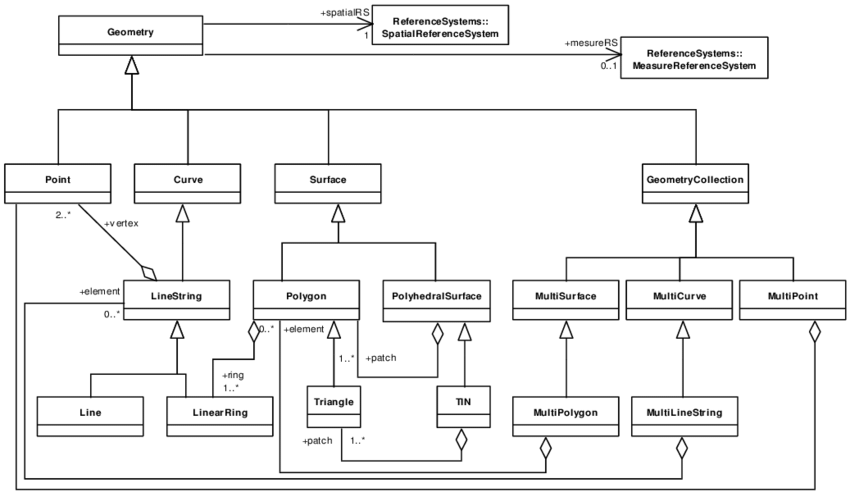
\includegraphics[width=1\linewidth]{imagenes/capitulo4/The-classes-of-geometries-in-WKT-figure-from-4}
	\caption{Jerarquía de clases \cite{estandar}}
	\label{fig:the-clases-geometry}
\end{figure}

Entonces, la figura \ref{fig:the-clases-geometry} muestra el modelo de objetos para la geometría de entidad simple usando la notación UML. La clase de \textit{Geometry} tiene subclases para \textit{Point}, \textit{Curve}, \textit{Surface} y \textit{GeometryCollection}, en donde cada objeto geométrico está asociado a un sistema de referencia espacial, que describe el espacio de coordenadas en el que se define el objeto geométrico \cite{estandar}. Para comprender mejor las clases representadas, vamos a ver una pequeña definición de cada una de ellas \cite{wkt-database} (figura \ref{fig:ejemplos}):

% La Figura 1 se basa en un modelo de Geometría extendida con clases especializadas de colección de 0, 1 y 2 dimensiones llamadas MultiPoint, MultiLineString y MultiPolygon para modelar geometrías correspondientes a colecciones de Puntos, LineStrings y Polígonos, respectivamente. MultiCurve y MultiSurface se presentan como superclases que generalizan las interfaces de colección para manejar Curvas y Superficies. La Figura 1 muestra líneas de agregación entre las clases de recolección de hojas y sus clases de elementos; Las líneas de agregación para las clases que no son de recolección de hojas se describen en el texto. Las colecciones no homogéneas son instancias de GeometryCollection.

\begin{itemize}
	\item \textit{\textbf{Point}}: representa una ubicación única en el espacio de coordenadas, tiene valores de coordenadas $x$ e $y$.
	
	\item \textit{\textbf{Curve}}: es una geometría unidimensional. 
	
	\item \textit{\textbf{LineString}}: es un subtipo de la clase \textit{Curve}, no tiene intersecciones propias y es cerrada si su punto de inicio es igual a su punto final.
	
	\item \textit{\textbf{Line}}: \textit{LineString} con exactamente dos puntos. 
	
	\item \textit{\textbf{LinearRing}}: \textit{LineString} cerrada y simple. 
	
	\item \textit{\textbf{Surface}}: es una geometría bidimensional (p.e. polígono con agujeros).% Esta clase es abstracta. %(es decir, no puede ser instanciada). %Una superficie simple puede consistir en un solo "parche" que tiene un límite "exterior" y 0 o más límites "interiores" (por ejemplo, un polígono con agujeros) .
	
	\item \textbf{Polygon}: \textit{Surface} simple plana que tiene exactamente un límite exterior y puede tener varios límites interiores que no se cruzan. %Cada polígono está topológicamente cerrado y no se cruzan dos límites. 
	
	\item \textit{\textbf{Triangle}}: es un \textit{Polygon} con 3 vértices distintos no colineales y sin límite interior. 
	
	\item \textbf{\textit{Polyhedral Surface}}: es una colección contigua de \textit{Polygon} que comparten segmentos límite comunes. %Cada par de polígonos que tocan tienen un límite común que se expresa como una colección finita de cadenas de líneas. 
	
	\item \textit{\textbf{Triangulated Irregular Network}}: un conjunto de puntos de triangulación para representar superficies en 3D.
	
	\item \textit{\textbf{Geometry Collection}}:  es un conjunto de geometrías distintas. 
		
	\item \textit{\textbf{MultiPoint}}: esta es una colección de geometría cuyos elementos son \textit{Point} que no están conectados.
	
	\item \textit{\textbf{MultiCurve}}: es una colección de geometría con elementos son \textit{Curve}.
	
	\item \textit{\textbf{MultiLineString}}: es una colección de geometría cuyos elementos son \textit{LineString}. 
	
	\item \textit{\textbf{MultiSurface}}: es una colección de geometría bidimensional cuyos elementos son \textit{Surface}.  
	
	\item \textit{\textbf{MultiPolygon}}: es una colección de superficies múltiples cuyos elementos son polígonos. Los límites de cada polígono pueden no cruzarse.
	
\end{itemize}

\begin{figure}[H]
	\centering
	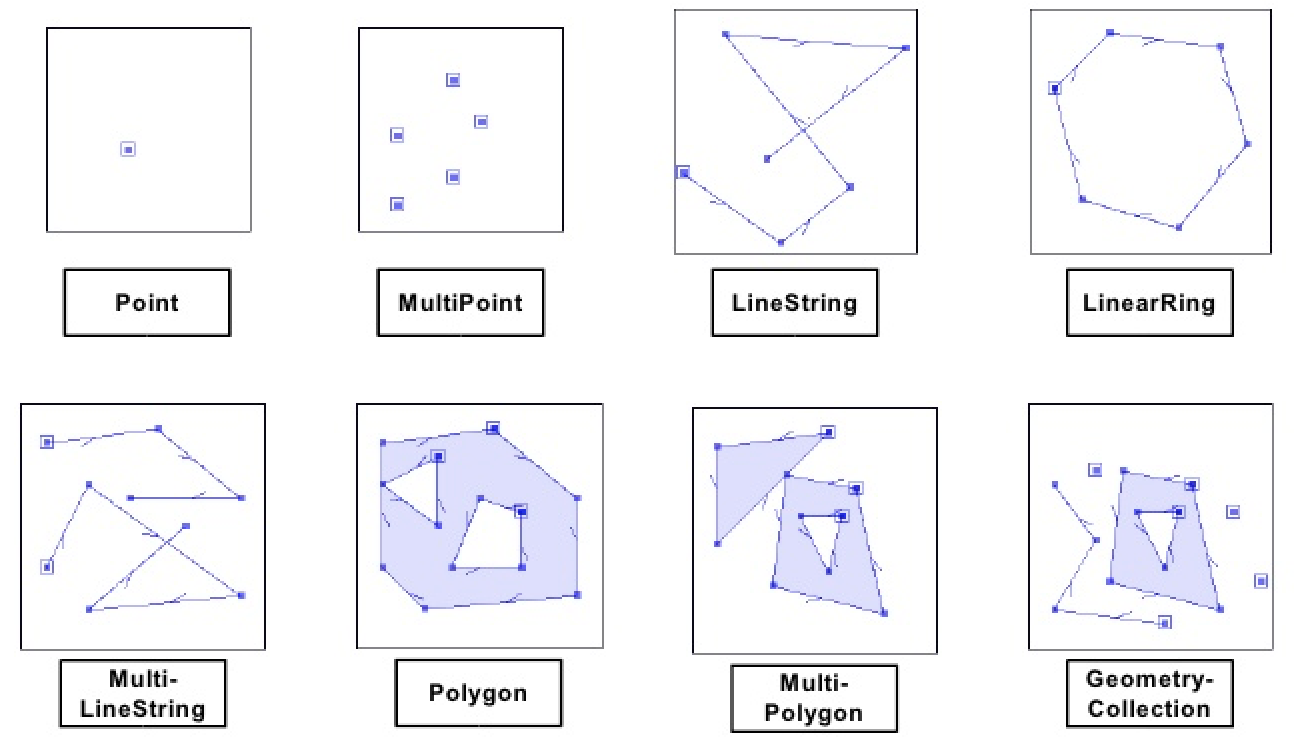
\includegraphics[width=0.9\linewidth]{imagenes/capitulo4/ejemplos}
	\caption{\textit{OpenGIS Simple Features Access} \cite{imagen-ejemplos}}
	\label{fig:ejemplos}
\end{figure}

Una vez que hemos definido las clases que componen el estándar, es necesario conocer las operaciones para las relaciones espaciales de la clase \textit{Geometry} (figura \ref{fig:geometry-class}).

\begin{figure}[H]
	\centering
	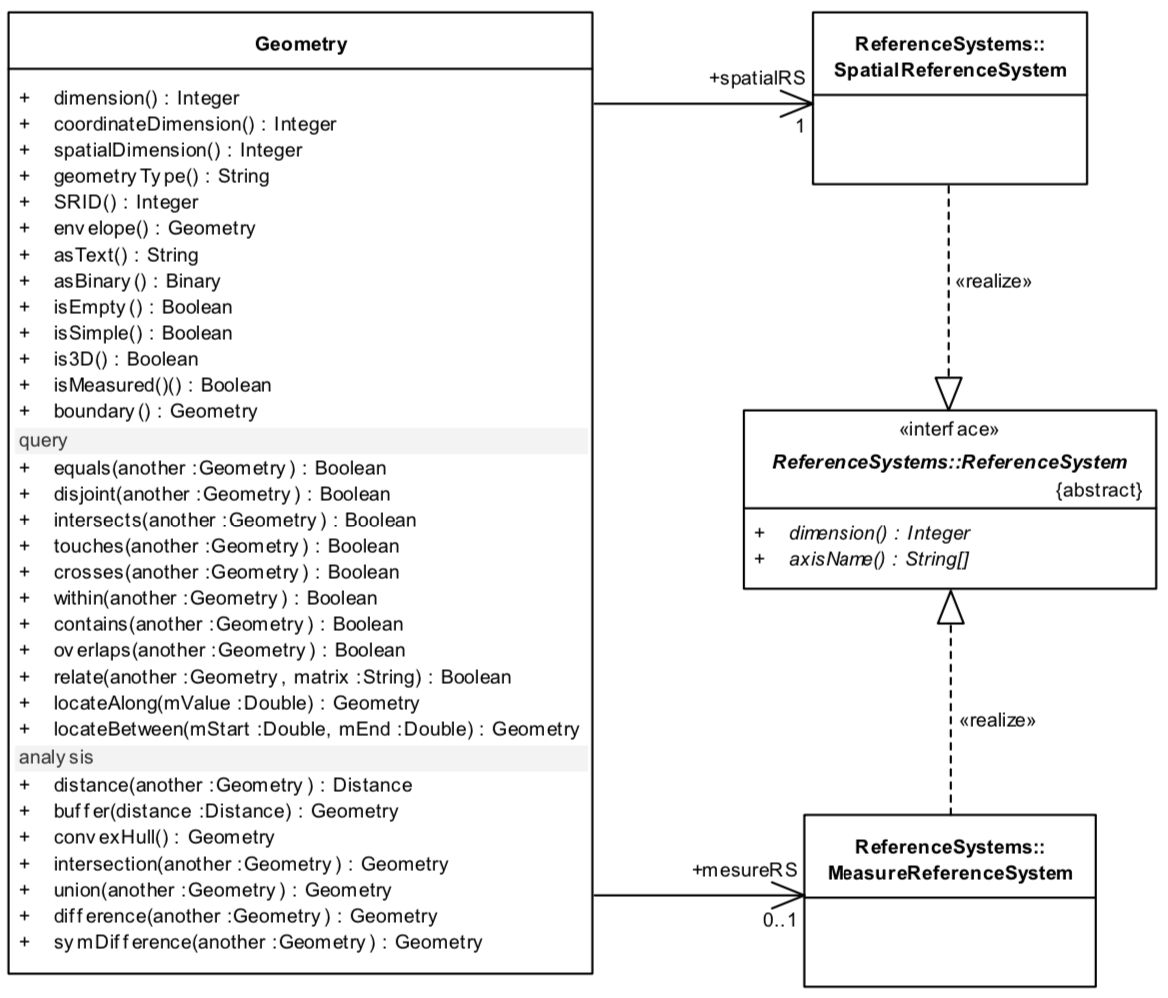
\includegraphics[width=1\linewidth]{imagenes/capitulo4/geometry-class}
	\caption{Operaciones de la clase \textit{Geometry} \cite{estandar}}
	\label{fig:geometry-class}
\end{figure}

\subsubsection{Operadores Booleanos de relaciones espaciales}

Comecemos por los \textbf{métodos para probar las relaciones espaciales entre objetos geométricos} de la clase \textit{Geometry}. Para cada uno de los métodos de la tabla \ref{estandar-funciones}), el tipo de retorno es entero, pero se interpreta como booleano, VERDADERO = 1, FALSO = 0. Corresponde a la parte de \texttt{query} de la figura \ref{fig:geometry-class} \cite{estandar, wkt-database}.



\subsubsection{Métodos de apoyo al análisis espacial}

Por otro lado los \textbf{métodos que apoyan el análisis espacial} de la clase \textit{Geometry} son análisis geométricos que dependen de la precisión de las representaciones de coordenadas y las limitaciones de la interpolación lineal en este estándar. La precisión del resultado a un buen nivel estará limitada por estos y otros problemas relacionados (tabla \ref{estandar-metodos}). Corresponde a la parte de \texttt{analysis} de la figura \ref{fig:geometry-class} \cite{estandar}.
 

 
 \begin{table}[H]
 	\caption{Operadores Booleanos de relaciones espaciales}
 	\label{estandar-funciones}
 	\centering
 	\begin{tabular}{|l|m{9.5cm}|}
 		\hline
 		\rowcolor[HTML]{EFEFEF} 
 		{\textbf{OPERADOR}} & { \textbf{DESCRIPCIÓN}} \\ \hline
 		\texttt{Equals}	&    \texttt{(anotherGeometry: Geometry): Integer} - Devuelve 1 (VERDADERO) si este objeto geométrico es ``espacialmente igual'' a otra \textit{Geometry}        \\ \hline
 		\texttt{Disjoint}	&       \texttt{(anotherGeometry: Geometry): Integer} - Devuelve 1 (VERDADERO) si este objeto geométrico es ``espacialmente disjunto'' de otra \textit{Geometry}              \\ \hline
 		\texttt{Intersects}	&   \texttt{(anotherGeometry: Geometry): Integer} - Devuelve 1 (VERDADERO) si este objeto geométrico ``se cruza espacialmente'' con otra \textit{Geometry}        \\ \hline
 		\texttt{Touches} &     \texttt{(anotherGeometry: Geometry): Integer} - Devuelve 1 (VERDADERO) si este objeto geométrico ``toca espacialmente'' otra \textit{Geometry}   (figura \ref{fig:touches})     \\ \hline
 		\texttt{Within}	&    \texttt{(anotherGeometry: Geometry): Integer} - Devuelve 1 (VERDADERO) si este objeto geométrico está ``espacialmente dentro'' de otra \textit{Geometry} (figura \ref{fig:within})               \\ \hline
 		\texttt{Contains} &     \texttt{(anotherGeometry: Geometry): Integer} -  Devuelve 1 (VERDADERO) si este objeto geométrico ``contiene espacialmente'' otra \textit{Geometry}      \\ \hline
 		\texttt{Overlaps}	&     \texttt{(anotherGeometry: Geometry): Integer} - Devuelve 1 (VERDADERO) si este objeto geométrico ``se superpone espacialmente'' a otra \textit{Geometry}         \\ \hline
 		\texttt{Crosses} &    \texttt{(anotherGeometry: Geometry): Integer} - Devuelve 1 (VERDADERO) si este objeto geométrico ``cruza espacialmente'' otra \textit{Geometry}    \\ \hline	
 		%\texttt{Relate} &   Devuelve 1 (VERDADERO) si este objeto geométrico está espacialmente relacionado con otra \textit{Geometry} probando las intersecciones entre el interior, el límite y el exterior de los dos objetos geométricos       \\ \hline	
 	\end{tabular}
 \end{table}

 \begin{figure}[H]
	\centering
	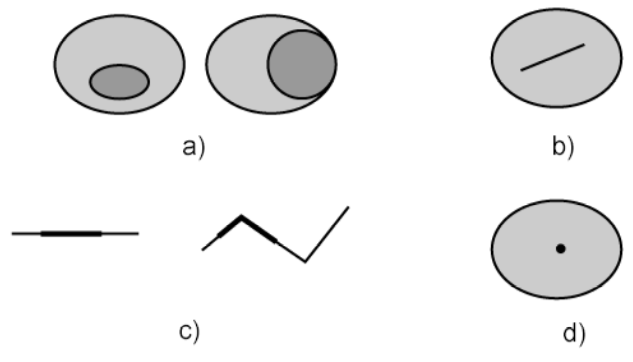
\includegraphics[width=0.7\linewidth]{imagenes/capitulo4/within}
	\caption{Ejemplos del operador \textit{Within} \cite{estandar}}
	\label{fig:within}
\end{figure}

 \begin{figure}[H]
 	\centering
 	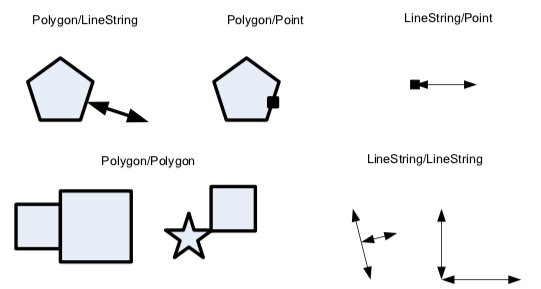
\includegraphics[width=0.71\linewidth]{imagenes/capitulo4/touches1}
 	\caption{Ejemplos del operador \textit{Touches} \cite{estandar}}
 	\label{fig:touches}
 \end{figure}


\begin{table}[H]
	\caption{Métodos de apoyo al análisis espacial}
	\label{estandar-metodos}
	\centering
	\begin{tabular}{|l|m{8.6cm}|}
		\hline
		\rowcolor[HTML]{EFEFEF} 
		{\textbf{FUNCIÓN} } & {\textbf{DESCRIPCIÓN}} \\ \hline
		\texttt{Distance}		&     \texttt{(anotherGeometry: Geometry):Double} - Devuelve la distancia más corta entre dos puntos de dos objetos geométricos        \\ \hline
		\texttt{Buffer} &     \texttt{(distance: Double): Geometry} -    Devuelve un objeto geométrico que representa todos los puntos cuya distancia desde este objeto geométrico es menor o igual que la distancia (figura \ref{fig:ejemplos-metodos} a)            \\ \hline
		\texttt{ConvexHull}	& \texttt{( ): Geometry} -     Devuelve un objeto geométrico que representa el casco convexo de este objeto geométrico (figura \ref{fig:ejemplos-metodos} b)             \\ \hline
		\texttt{Intersection} &   \texttt{(anotherGeometry: Geometry): Geometry} -    Devuelve un objeto geométrico que representa la intersección del conjunto de puntos de este objeto geométrico con otra \textit{Geometry}            \\ \hline
		\texttt{Union}	&  \texttt{(anotherGeometry: Geometry): Geometry}	-    Devuelve un objeto geométrico que representa la unión del conjunto de puntos de este objeto geométrico con otra \textit{Geometry}              \\ \hline
		\texttt{Difference} &  \texttt{(anotherGeometry: Geometry): Geometry } -  Devuelve un objeto geométrico que representa la diferencia de conjunto de puntos de este objeto geométrico con otra \textit{Geometry}            \\ \hline
		\texttt{SymDifference}	&   \texttt{(anotherGeometry: Geometry): Geometry}  - Devuelve un objeto geométrico que representa la diferencia simétrica del conjunto de puntos de este objeto geométrico con otra \textit{Geometry}                 \\ \hline
	\end{tabular}
\end{table}

\begin{figure}[H]
	\centering
	\begin{subfigure}[h]{0.32\textwidth} 
		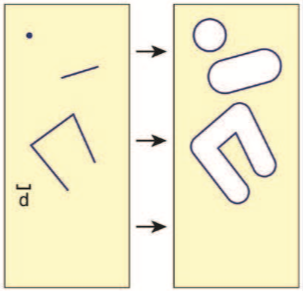
\includegraphics[width=\textwidth]{imagenes/capitulo4/buffer}
		\caption{\textit{Buffer}}
	\end{subfigure}       
	\begin{subfigure}[h]{0.32\textwidth} 
		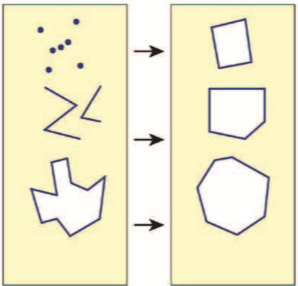
\includegraphics[width=\textwidth]{imagenes/capitulo4/convexHull}
		\caption{\textit{ConvexHull}}
	\end{subfigure}
	\caption{Ejemplos de los métodos \cite{AsignaturaSIG}}
	\label{fig:ejemplos-metodos}
\end{figure}



 


Con esto acabamos de definir los métodos y las funciones para manejar las subclases de las clases de \textit{Geometry}. A continuación, vamos a definir GeoSPARQL, lenguaje de consulta geoespacial muy relacionado con el estándar aquí expuesto.

\subsection{GeoSPARQL}

% tesis
% libro
\textbf{GeoSPARQL} es un estándar establecido por \textit{Open Geoespatial Consortium} (OGC). Es un lenguaje de consulta basado en SPARQL para recuperar información geoespacial de conjuntos de datos RDF en la Web Semántica \cite{libro-gis}. GeoSPARQL define gran parte de lo que se requiere para un lenguaje de consulta de este tipo al proporcionar vocabulario (clases, propiedades y funciones) que se pueden utilizar en gráficos RDF y consultas SPARQL para representar y consultar datos geoespaciales (figura \ref{fig:geosparql}). GeoSPARQL sigue el diseño modular típico de los estándares OGC \cite{ogc-geo, wkt-database}.

%Entre sus características podemos encontrar \cite{ogc-geo}: 
%\begin{itemize}
%	\item Vocabulario RDF/OWL para representar información geoespacial.
%	\item Funciones extensión a SPARQL para cálculos espaciales.
%	\item Conjunto básico de clases, propiedades y tipo de datos que son utilizados para construir patrones de consulta (figura \ref{fig:geosparql}). 
%\end{itemize}

\begin{figure}[H]
	\centering
	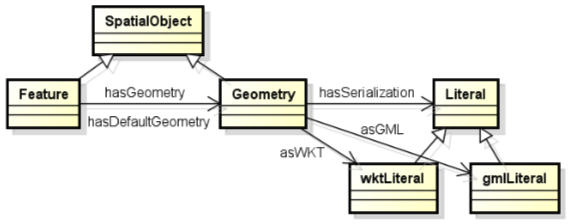
\includegraphics[width=0.9\linewidth]{imagenes/capitulo3/geosparql}
	\caption{Clases y propiedades básicas de GeoSPARQL \cite{tesis-otro}}
	\label{fig:geosparql}
\end{figure}

GeoSPARQL no define un vocabulario completo para representar información espacial, sino que define un conjunto central de clases, propiedades y tipos de datos que se pueden utilizar para construir patrones de consulta (figura \ref{fig:geosparql}) \cite{ogc-geo}. Es un lenguaje muy enfocado para la comunidad SIG. Por otro lado, para poder hacer uso de este tipo de consultas es necesario aplicar las especificaciones del estándar que vienen descritas en la documentación oficial\footnote{\url{https://www.opengeospatial.org/standards/geosparql}}. En la tabla \ref{topo-geosparql} podemos encontrar sus relaciones topológicas, mientras que en la tabla \ref{funciones-geosparql} podemos encontrar funciones de GeoSPARQL que incluyen alternativas de todas las propiedades de relación topológica, aplicadas como funciones en literales de geometría \cite{tesis-otro}. \\

Una decisión de diseño crucial de GeoSPARQL es usar valores literales para codificar geometrías como una sola unidad (puntos, líneas y polígonos,) e introducir dos tipos de datos RDF \texttt{geo:wktLiteral} y \texttt{geo:gmlLiteral} para estos literales. Dicha extensión está parametrizada por el estándar de serialización de OGC para codificar literales de geometría (WKT o GML). En nuestro caso, como ya hemos ido comentando vamos hacer uso del literal  \texttt{geo:wktLiteral}. \texttt{wktLiteral} consiste en un URI opcional que identifica el sistema de referencia de coordenadas seguido de la codificación WKT de una geometría, por ejemplo \cite{wkt-database}: 

\begin{lstlisting}
# Primera manera para representar el literal wktLiteral
"POINT(-83.38 33.95)"^^geo:wktLiteral

# Segunda manear para representar el literal wktLiteral
"<http://www.opengis.net/def/crs/EPSG/0/4326>
POINT(33.95 -83.38)"^^geo:wktLiteral
\end{lstlisting}

%Respecto la geometría permite puntos, líneas y polígonos, como vimos en el capítulo anterior y además la representación de la geometría debe de estar codificada en formato WKT 

\begin{table}[H]
	\caption{Relaciones topológicas con sus significados}
	\label{topo-geosparql}
	\centering
	\begin{tabular}{|l|l|}
		\hline
		\rowcolor[HTML]{EFEFEF} 
		{\textbf{OBJETO}} & { \textbf{DESCRIPCIÓN}} \\ \hline
		\texttt{sfEquals}	&              Espacialmente igual           \\ \hline
		\texttt{sfDisjoint}	&        Disjunto (no puede tocar)                 \\ \hline
		\texttt{sfIntersects}	&     Comparten al menos un punto                    \\ \hline
		\texttt{sfTouches} &          Se tocan externamente               \\ \hline
		\texttt{sfWithin}	&      Está dentro (puede tocar el límite)                   \\ \hline
		\texttt{sfContains} &             El inverso de \texttt{sfWithin}            \\ \hline
		\texttt{sfOverlaps}	&            Tienen algunos puntos comunes, misma dimensión             \\ \hline
		\texttt{sfCrosses} &         Por ejemplo, área cruza la línea                \\ \hline		
	\end{tabular}
\end{table}


También se definen propiedades para representar metadatos de geometrías (por ejemplo, \textit{geo:dimension} que captura la dimensión topológica) o para asociar geometrías con sus literales (\textit{geo:asWKT}). Además, esta extensión define funciones para realizar operaciones no topológicas en geometrías (por ejemplo, \textit{geof:distancie} o \textit{geof:ConvexHull}), las cuales son las mismas definidas anteriormente por el estándar \cite{wkt-database}.


\begin{table}[H]
	\caption{Funciones para comparar y manipular geometrías}
	\label{funciones-geosparql}
	\centering
	\begin{tabular}{|l|m{8.6cm}|}
		\hline
		\rowcolor[HTML]{EFEFEF} 
		{\textbf{FUNCIÓN} } & {\textbf{DESCRIPCIÓN}} \\ \hline
		\texttt{distance}		&       La distancia de dos literales geométricos medidos en unidades dadas                  \\ \hline
		\texttt{buffer} &           Literal de geometría como un literal de entrada con un buffer agregado, dado el radio y las unidades del buffer              \\ \hline
		\texttt{convexHull}	&      El casco convexo de un literal de geometría                   \\ \hline
		\texttt{intersection} &          La intersección de dos literales de geometría               \\ \hline
		\texttt{union}		&     Unión de dos literales de geometría                    \\ \hline
		\texttt{difference} &       La diferencia de dos literales de geometría                  \\ \hline
		\texttt{symDifference}	&      Establecer la diferencia simétrica de dos literales de geometría                  \\ \hline
		\texttt{envelope}  &              El cuadro delimitador de un literal de geometría           \\ \hline
		\texttt{boundary}		&    El límite de un literal de geometría                     \\ \hline
		\texttt{getsrid} &       URI del sistema de referencia espacial de un literal de geometría                  \\ \hline		
	\end{tabular}
\end{table}

En el apartado siguiente, haremos uso de este lenguaje para la obtención de la información geoespacial deseada, centrándonos en varios ejemplos prácticos, y su uso de cara al futuro.

\section{Conclusiones}

Este capítulo ha introducido el estándar usado en el lenguaje de consulta geoespacial GeoSPARQL, como nexo de unión de las áreas de los SIG y la Web Semántica. Se ha apreciado, que las funciones usadas en el GeoSPARQL son las mismas que OGC ha definido en su estándar. Con esto acabamos de comprobar como ha sido posible unir dos ámbitos que previamente parecían ser independientes el uno respecto del otro.
\chapter{Web Semántica Geoespacial}
\label{ch:aplicacion}

\begin{quote}
	{\bf\textsc{Resumen:}} Este capítulo presenta la prueba de concepto realizada para la incorporación de Información Geográfica, procedente de Ogíjares (Granada), mediante herramientas de la Web Semántica. En el ejemplo se estudian y proponen herramientas de la Web Semántica que se pueden utilizar para representar e integrar datos geoespaciales con diferentes geometrías.
\end{quote}



\section{Prueba de Concepto}

Como hemos comentado, uno de nuestros objetivos es estudiar las herramientas de la Web Semántica que se pueden utilizar para representar e incorporar Información Geográfica, valorarlas y desarrollar una prueba de concepto. Para ello es necesario haber entendido los capítulos dedicados a los sistemas SIG y a la Web Semántica, y así comprender que el principal nexo de unión entre ambas tecnologías es la estandarización de las operaciones y funciones usadas en las consultas de GeoSPARQL; tal y como hemos visto en el anterior capítulo. Conociendo todos estos conceptos es posible comenzar con el desarollo de la ontología GEOARES, sin embargo, la primera tarea imprescindible es la selección del conjunto de datos geoespaciales que se desea hacer accesible mediante la Web Semántica. \\

Durante la prueba de concepto contaremos con la presencia de las herramientas destinadas a la generación de información geoespacial con \texttt{QGIS}, para permitir obtener la información de los \textit{Shapefile} a hojas de cálculo; generación de documentos \textit{RDF} con \texttt{Protegé}, para permitir llevar la información de los \textit{Shapefile} hacia documentos en formato \textit{RDF} de manera gráfica; consumo con \texttt{GraphBD},  para permitir la visualización de archivos en formato \textit{RDF} y la realización de las consultas con el lenguaje estándar de consulta geoespacial \textit{GEOSPARQL}; y visualización de la información geoespacial obtenida de las consultas con \texttt{R} para permitir ubicar la información geográfica en un mapa interactivo mediante la librería \textit{Shiny}.\\


% \texttt{QGIS} para permitir obtener la información de los \textit{Shapefile} a hojas de cálculo, generación de documentos \textit{RDF}  mediante \texttt{Protegé} para permitir llevar la información de los \textit{Shapefile} hacia documentos en formato \textit{RDF} de manera gráfica y su posterior visualización), consumo (mediante \texttt{GraphBD} para permitir la visualización de archivos en formato \textit{RDF} y la realización de las consultas del lenguaje estándar de consulta geoespacial \textit{GEOSPARQL}) y visualización de la información geoespacial obtenida de las consultas (\texttt{R} para permitir ubicar la información geográfica en un mapa interactivo mediante la librería \textit{Shiny}). 

\textit{\textbf{Nota}: La versión usada de QGIS es la 3.8.0-Zanzibar, la version de R es la 3.6.1, la versión de Protegé es la 5.5.0 y la versión de GraphDB Free es la 8.10.1, softwares usado en un macOS 10.14}

\subsection{Selección y obtención de los datos geográficos}

En la actualidad, disponemos de diversas fuentes oficiales y no oficiales que nos proporcionan mapas de calidad con los que poder trabajar. No obstante, al querer hacer uso de Información Geográfica de España, es importante destacar dos fuentes principales:

\begin{itemize}
	\item \textbf{Instituto Geográfico Nacional (IGN)}, es la fuenta oficial para todo el territorio español y la descarga de mapas se puede realizar a través de la dirección \url{http://centrodedescargas.cnig.es/CentroDescargas/buscador.do#}.
	
	\item \textbf{Instituto de Estadística y Cartografía de Andalucía}, es la fuente oficial para todo el territorio andaluz y la descarga de mapas se puede realizar a través de la dirección \url{https://www.juntadeandalucia.es/institutodeestadisticaycartografia/bcadescargas/}.
\end{itemize}
 
Sin embargo, como vamos a trabajar con datos procedentes de la provincia de Granada, en concreto de mi pueblo Ogíjares, he optado por escoger los que nos proporciona el \textit{Instituto de Estadística y Cartografía de Andalucía} \cite{base-andalucia}. A continuación, se muestran los pasos para su obtención:

\begin{enumerate}
	
		\begin{figure}[H]
		\centering
		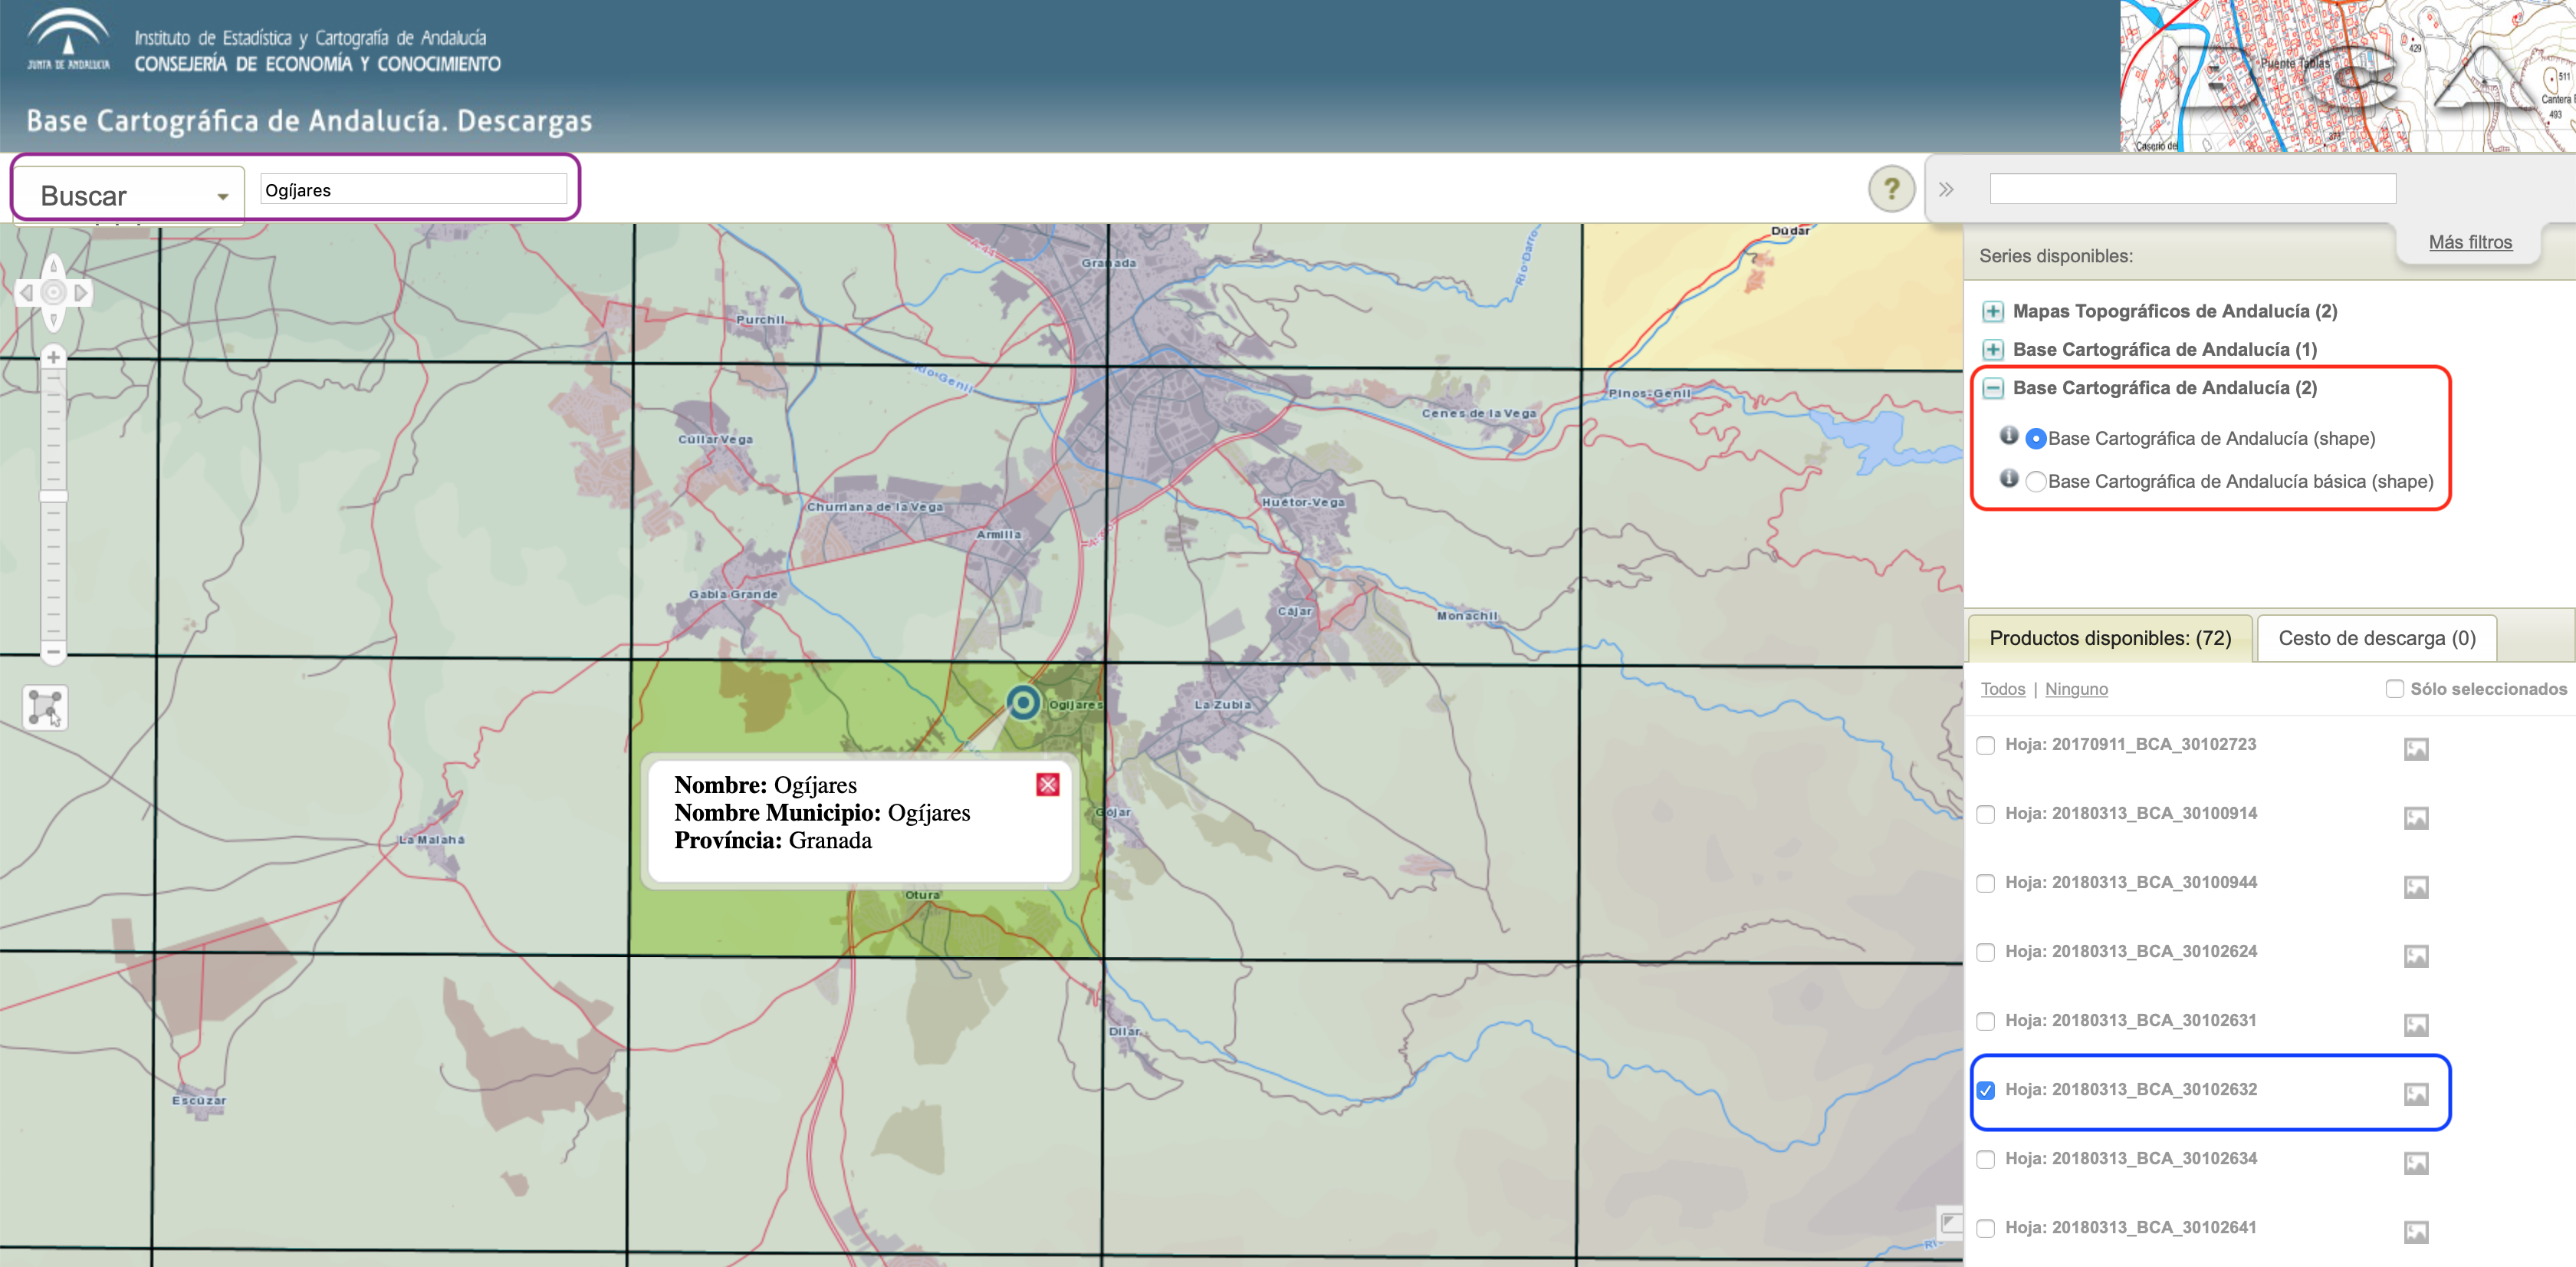
\includegraphics[width=1\linewidth]{imagenes/capitulo5/obtencion-informacion}
		\caption{Portal del Instituto de Estadística y Cartografía \cite{base-andalucia}}
		\label{fig:obtencion-informacion}
	\end{figure}

	\item La descarga se realiza a través de la plataforma del Instituto de Estadística y Cartografía de Andalucía, de la Consejería de Economía y Conocimiento (URL mencionada en el punto anterior). Una vez dentro, seleccionamos la opción \textit{Base Cartográfica de Andalucía (2)}, escogemos \textit{Base Cartográfica de Andalucía (shape)} y buscamos el municipio de \textit{Ogíjares} (figura \ref{fig:obtencion-informacion}). Nos aparecerán varios cuadrantes, escogemos con el que nosotros queramos trabajar; yo me he descargado el cuadrante que aparece seleccionado y remarcado en color, asociado a mi pueblo Ogíjares.
	
		\item La carpeta descargada contiene mapas de áreas muy diversas, las cuales hacen uso de geometría de punto, de línea o de área. Entre las capas que se nos proporciona nos podemos encontrar diversos modelos de datos (tabla \ref{elementos-mapas}). \textit{Si queremos saber más sobre de cada uno de ellos debemos acceder al siguiente \underline{\href{https://www.juntadeandalucia.es/institutodeestadisticaycartografia/prodCartografia/bc/modelo/00_Modelo_Datos_Base_Cartografica_Andalucia.pdf}{enlace}}.}
		



	
	
	
	\begin{table}[H]
		\caption{Esquema del modelo de datos descargado}
		\label{elementos-mapas}
		\centering
		\begin{tabular}{|m{6.2cm}|m{5.4cm}|}
			\hline
			\rowcolor[HTML]{EFEFEF} 
			\textbf{MODELO DE DATOS} & \textbf{ELEMENTOS} \\ \hline
			\textsc{Infraestructuras geográficas}&  Líneas administrativas            \\ \hline
			\textsc{Toponimia}&              Topónimos      \\ \hline
			\textsc{Relieve}&         Curvas de nivel, puntos de cota           \\ \hline
			\textsc{Sistema urbano}&       Edificaciones, curvas artificiales             \\ \hline
			\textsc{Servicios}&       Centros educativos o deportivos             \\ \hline
			\textsc{Red hidrográfica}&       Corriente artificial, punto fluvial  \\ \hline
			\textsc{Red viaria}&      Carreteras, carril bici              \\ \hline
			\textsc{Infraestructuras energéticas y de telecomunicaciones}&     Instalación de energía eléctrica, explotación minera               \\ \hline
			\textsc{Infraestructuras hidráulicas}&     Depósitos hidráulicos, presas               \\ \hline
			\textsc{Infraestructuras de transportes} &         Área de servicio de descanso       \\ \hline
			\textsc{Infraestructuras medioambientales} &     Instalación de tratamiento de aguas.               \\ \hline
			\textsc{Cubierta terrestre}&           Lindes        \\ \hline
		\end{tabular}
	\end{table}
	
		\begin{figure}[H]
		\centering
		
\includegraphics[width=1\linewidth]{imagenes/capitulo2/shapefile}
		\caption{Diferentes archivos que componen el formato Shapefile }
		\label{fig:shapefile}
	\end{figure}
	
	\item El fichero descargado para cada uno de los modelos de datos que acabamos de comentar tiene como formato principal \textit{Shapefile (sh)}, el formato más usado para almacenar información geoespacial. Es un formato de archivos que almacena información no topológica con características espaciales de elementos geográficos que soportan geometrías como puntos, líneas y polígonos \cite{tesis}.  Es originario de \textit{Enviromental Systems Research Institute} (ESRI)\footnote{Empresa que desarolla y comercializa software para SIG.} y consta fundamentalmente de un archivo principal, un archivo de índice y una tabla dBase. Estos archivos suelen requerir poco espacio de almacenamiento en disco y se pueden leer y escribir con facilidad. Los diferentes archivos que componen el formato Shapefile tienen el mismo nombre cada uno con su respectiva extensión, como se aprecia en la figura \ref{fig:shapefile}:
	


	\begin{itemize}
		\item \textbf{Archivo principal (*.shp)}: archivo de longitud variable en el que cada registro describe una forma con sus respectivos vértices. 
		
		\item \textbf{Archivo de índice (*.shx)}: acompaña al archivo principal (*.shp) que almacena la posición de los identificadores de entidades individuales en el archivo .shp 
		
		\item \textbf{Tabla dBase (*.dbf)}: almacena la información de atributos de las entidades. 
	\end{itemize}	

	\begin{figure}[H]
	\centering
	\includegraphics[width=0.6\linewidth]{imagenes/capitulo5/codificacion}
	\caption{Sistema de referencia usado en los Shapefiles}
	\label{fig:codificacion}
\end{figure}

	\item La visualización del archivo Shapefile se puede realizar a través de cualquier software SIG, en nuestro caso vamos a utilizar el software de análisis geoespacial QGIS. Respecto los modelos de datos disponibles que se desean escoger para hacer accesible mediante la Web Semántica, vamos a centrarnos en la información geoespacial de edificaciones, curvas de nivel y puntos de cota de Ogíjares (Granada) \cite{info-sh}, basados en el sistema de referencia ETRS89 (figura \ref{fig:codificacion}).
	

	

	

	\begin{itemize}
		\item \textbf{Edificaciones}: se agrupan en esta capa varios elementos que conforman edificaciones con geometría de polígono (figura \ref{fig:edificaciones}). Dispone de la información:
		
		\begin{itemize}
			\item \textsc{GID}.	
			\item \textsc{ID de la hoja}.
			\item \textsc{Estado}: estado de uso de la entidad o el tramo de la entidad.
			\begin{itemize}
				\item 	\small{En construcción (CON), en ruinas (RUI), sin clasificar (SCL) o en uso (USO).}
			\end{itemize}
			
			\item \textsc{Tipo}: tipo de elemento según su función.
			\begin{itemize}
				\item 	\small{Caseta o cobertizo (CAS), caso genérico (CGN), chabola (CHA), chimenea (CHI), edificación (EDI), industrial (IND), invernadero (INV), marquesina (MAR), nave abierta (NAB), nicho (NIC), patio (PAT), sin clasificar (SCL), tentadero (TEN), torre genérica (TGN), transformador (TRF) o torre de vigía (TVG).}
			\end{itemize}
			 
		\end{itemize}
	
		\begin{figure}[H]
		\centering
		\includegraphics[width=0.92\linewidth]{imagenes/capitulo5/edificaciones}
		\caption{Visualización del elemento \textit{Edificaciones} en QGIS}
		\label{fig:edificaciones}
	\end{figure}

		
		
		\item \textbf{Curvas de nivel}: línea imaginaria de altitud constante que sirve para describir la forma tridimensional de la superficie terrestre con geometría de línea (figura \ref{fig:curvasnivel}). Dispone de la información:
		
		\begin{itemize}
			\item \textsc{GID}.	
			\item \textsc{ID de la hoja}.
			\item \textsc{Cota}: recoge la coordenada altura ortométrica del elemento capturado en metros.
			\item \textsc{Categoría}: categoría de la curva de nivel.
			\begin{itemize}
				\item 	\small{Auxiliar (AUX), maestra (MAE), normal (NOR) o sin clasificar (SCL).}
			\end{itemize}
			
			\item \textsc{Procedencia}: procedencia de la curva de nivel.
			\begin{itemize}
				\item 	\small{Combinado (CMB), elementos terreno (ETE), lidar (LID), MDT (MDT), restitución (RES) o sin clasificar (SCL).}
			\end{itemize} 
			\item \textsc{Tipo}: tipo de la curva de nivel.
			\begin{itemize}
				\item 	\small{Caso genérico (CGN), depresión (DEP) o sin clasificar (SCL).}
			\end{itemize}
			
		\end{itemize}
	
	\begin{figure}[H]
		\centering
		\includegraphics[width=0.92\linewidth]{imagenes/capitulo5/curvasnivel}
		\caption{Visualización del elemento \textit{Curvas de Nivel} en QGIS}
		\label{fig:curvasnivel}
	\end{figure}
		
		
		
		
		\item \textbf{Punto cota}: punto situado sobre la superficie terrestre del cual se conoce su altitud sobre el nivel medio del mar, y que se representa para facilitar la interpretación gráfica de la morfología del terreno con geometría de punto (figura \ref{fig:puntocota}). Dispone de la información:
		
		\begin{itemize}
			\item \textsc{GID}.	
			\item \textsc{ID de la hoja}.
			\item \textsc{Cota}: recoge la coordenada altura ortométrica del elemento capturado en metros.
			\item \textsc{Contexto}: contexto del punto de cota.
			\begin{itemize}
				\item 	\small{Caso genérico (CGN), cima (CIM), collado (COL), depresión (DEP), edificación (EDI) o sin clasificar (SCL).}
			\end{itemize}
		\end{itemize}

		\item \textsc{Tipo}: tipo de elemento según su función.
		
		\begin{itemize}
			\small{
			\item Punto cota construcción elevada (CON) o punto cota terreno (TER).
		}\end{itemize}
	\end{itemize}

	\begin{figure}[H]
		\centering
		\includegraphics[width=0.92\linewidth]{imagenes/capitulo5/puntocota}
		\caption{Visualización del elemento \textit{Punto Cota} en QGIS}
		\label{fig:puntocota}
	\end{figure}
\end{enumerate}

\begin{figure}[H]
	\centering
	\includegraphics[width=1\linewidth]{imagenes/capitulo5/mapa}
	\caption{Visualización de las tres geometrías en QGIS}
	\label{fig:mapa}
\end{figure}


Con esto hemos terminado de explicar los datos que vamos hacer accesibles a través de la Web Semántica. En la figura \ref{fig:mapa} es posible visualizar las tres geometrías juntas y localizadas en QGIS a través de la capa \textit{OpenStreetMap}, en donde las líneas verdes hacen referencia a las curvas de nivel, los puntos rojos a los puntos de cota y los polígonos azules a las edificaciones.\\

Al disponer de los datos listos para su uso, es necesario saber que para poblar una ontología con Protegé, se necesitan los datos geoespaciales en formato para CSV. Adicionalmente, como hemos visto, la representación de la ubicación de cada geometría la vamos a usar mediante la codificación WKT. No obstante, QGIS nos ofrece diversas funcionalidades, entre las que se encuentran las anteriores mencionadas y que nos permiten realizar el trabajo de una manera más sencilla.\\ 

%Se han propuesto otros esquemas para codificar datos de geometría simple en RDF. El vocabulario de Geografía básica del W3C (http://www.w3.org/2003/01/geo/) es un vocabulario popular. Estos vocabularios simples tienen limitaciones, por ejemplo, la incapacidad de especificar diferentes datos y sistemas de coordenadas, y por lo tanto no se usaron en GeoSPARQL. Tenga en cuenta que la mayoría de los datos de geometría existentes codificados con estos vocabularios se pueden convertir fácilmente en representaciones GeoSPARQL. La consulta SPARQL a continuación crea valores geo: wktLiteral a partir de geometrías de geografía básica del W3C.


%Esta sección establece los requisitos para representar datos de geometría en RDF basados en WKT según lo definido por Características simples [ISO 19125-1].

%Todos los literales RDFS de tipo geo: wktLiteral consistirán en un URI opcional que identifica el sistema de referencia de coordenadas seguido de Texto bien conocido de características simples (WKT) que describe un valor geométrico. Geo válido: wktLiterals se forman concatenando un URI absoluto válido como se define en [RFC 2396], uno o más espacios (carácter Unicode U + 0020) como separador y una cadena WKT como se define en Características simples [ISO 19125-1 ]

Para obtener el formato CSV en QGIS se realizar el mismo proceso en las tres capas: \textit{click derecho sobre la capa en cuestión, Exportar > Guardar objetos como} y nos aparecerá una ventana como la de la figura \ref{fig:csv}.

\begin{figure}[H]
	\centering
	\includegraphics[width=0.6\linewidth]{imagenes/capitulo5/csv}
	\caption{Obtener la información de los Shapefiles en CSV}
	\label{fig:csv}
\end{figure}

Además, para obtener la codificación WKT y poder hacer consultas a partir de la ubicación de las geometrías, debemos seleccionar en GEOMETRY la opción AS\_WKT (figura \ref{fig:opciones}). Por último, guardamos los CSV (figura \ref{fig:guardar}) y comprobamos que la salida es correcta (tablas \ref{csv-curva1}, \ref{csv-curvas2}, \ref{csv-poligonos} y \ref{csv-puntos}).


\begin{figure}[H]
	\centering
	\includegraphics[width=0.6\linewidth]{imagenes/capitulo5/opciones}
	\caption{Seleccionar opciones para guardar el Shapefile}
	\label{fig:opciones}
\end{figure}

\begin{figure}[H]
	\centering
	\includegraphics[width=0.6\linewidth]{imagenes/capitulo5/guardar}
	\caption{Guardando el fichero CSV de los Shapefiles}
	\label{fig:guardar}
\end{figure}

\begin{table}[H]
	\centering
	\caption{Parte del CSV para Edificaciones}
	\label{csv-poligonos}
	\begin{tabular}{|m{4cm}|c|c|c|c|}
		\hline
		\rowcolor[HTML]{EFEFEF} 
		\textbf{WKT}                        & \textbf{GID} & \textbf{ID} & \textbf{TIPO} & \textbf{ESTADO} \\ \hline
		POLYGON ((446020.74 4107035.28, ...)) & 181062       & 102632            & EDI           & USO                       \\ \hline
		POLYGON ((446050.16 4107127.71, ...))  & 181064       & 102632            & EDI           & USO                  \\ \hline
		POLYGON ((441430.69 4106827.08, ...)) & 758271       & 102632            & EDI           & USO                     \\ \hline
		...  & ...       & ...            & ...           & ...                     \\ \hline
		POLYGON ((446168.83 4108720.87, ... )) & 1330488       & 102632            & PAT           & CGN                    \\ \hline
	\end{tabular}
\end{table}

\begin{table}[H]
	\centering
	\caption{Parte del CSV para Puntos de Cota}
	\label{csv-puntos}
	\begin{tabular}{|m{3cm}|c|c|c|c|c|}
		\hline
		\rowcolor[HTML]{EFEFEF} 
		\textbf{WKT}                        & \textbf{GID} & \textbf{ID} & \textbf{TIPO} & \textbf{CONTEXTO} & \textbf{COTA} \\ \hline
		MULTIPOINT ((446228.92 4108432.53)) & 890947       & 102632            & TER           & CGN               & 721.77        \\ \hline
		MULTIPOINT ((446265.60 4108675.83))  & 890948       & 102632            & TER           & CGN               & 715.40        \\ \hline
		MULTIPOINT ((445197.65 4107245.48)) & 890949       & 102632            & TER           & CGN               & 761.02        \\ \hline
		...  & ...       & ...            & ...           & ...               &...        \\ \hline
		MULTIPOINT ((442401.99 4104501.95)) & 891529       & 102632            & TER           & CGN               & 771.75        \\ \hline
	\end{tabular}
\end{table}




\begin{table}[H]
	\centering
	\caption{Parte del CSV para Curvas de Nivel I}
	\label{csv-curva1}
	\begin{tabular}{|m{4.2cm}|c|c|c|c|}
		\hline
		\rowcolor[HTML]{EFEFEF} 
		\textbf{WKT} & \textbf{GID} & \textbf{ID} & \textbf{TIPO} & \textbf{CATEGORIA}  \\ \hline
		LINESTRING (440675.4 4106319.93, ....)       & 122602       & 102632            & CGN           & NOR                           \\ \hline
		LINESTRING (440972.5 4106237.28, ...)     & 172684       & 102632            & CGN           & NOR                       \\ \hline
		LINESTRING (440976.2 4106311.24, ...)              & 186391       & 102632            & CGN           & NOR                        \\ \hline
	...                                & ...       & ...            & ...           & ...                      \\ \hline
	
	LINESTRING (442507.6 4105386.75, ...)             & 471150       & 102632            & DEP           & MAE                       \\ \hline
	\end{tabular}
\end{table}

\begin{table}[H]
	\centering
	\caption{Parte del CSV para Curvas de Nivel II}
	\label{csv-curvas2}
	\begin{tabular}{|m{4.2cm}|c|c|c|}
		\hline
		\rowcolor[HTML]{EFEFEF} 
		\textbf{WKT}  & \textbf{PROCEDENCIA} & \textbf{COTA} \\ \hline
		LINESTRING (....)                  & CMB                 & 770           \\ \hline
		LINESTRING (...)                   & CMB                 & 780           \\ \hline
		LINESTRING (...)                      & CMB                 & 780           \\ \hline
		...                                & ...       & ...                  \\ \hline
		
		LINESTRING (...)                              & CMB                 & 750           \\ \hline
	\end{tabular}
\end{table}


Por tanto, la información que está contenida en la muestra de las anteriores tablas, contiene la información para poblar nuestra ontología, siendo necesario disponer de ellas en formato Excel.




\subsection{Creación de la ontología GEOARES}

Una vez seleccionado el conjunto de datos que se desea hacer accesible mediante la Web Semántica, es hora de pasar al desarrollo y creación de la ontología GEOARES. Gracias a la ontología es posible romper la barrera de la interoperabilidad, en donde los datos geoespaciales pueden ser utilizados por diferentes tipos de programas y aplicaciones. La interoperabilidad de los datos geoespaciales es extremadamente importante para las aplicaciones geoespaciales, ya que existen grandes cantidades de datos espaciales en diferentes formatos geográficos. La interoperabilidad de los datos geoespaciales elimina las barreras para el intercambio de datos y permite a los usuarios acceder, mapear, visualizar y analizar directamente datos con diferentes formatos. Los datos geoespaciales interoperables hacen posible la distribución rápida de información y el intercambio entre departamentos \cite{libro-gis}.\\

No obstante, escribir en lenguajes como RDF y OWL para la creación de la ontología resultan sumamente difícil y propensos a errores. Afortunadamente, existen en el mercado entornos gráficos para visualizar y construir ontologías de forma más fácil, como \textbf{Protegé} (figura \ref{fig:protege}). Es por eso que vamos hacer uso de este software para la creación de nuestra ontología.

\begin{figure}[H]
	\centering
	\includegraphics[width=1\linewidth]{imagenes/capitulo5/protege}
	\caption{Inicio de Protegé}
	\label{fig:protege}
\end{figure}

Hay que tener en cuenta que la ontología está enfocada para ser manejada en España y los datos obtenidos son procedentes de Andalucía, por lo cual las clases aparecerán en Español, a excepción de las que se nos especifique en GeoSPARQL según el estándar especificado. Básicamente una ontología geoespacial se basa en (figura \ref{fig:ontologia-geosparql}):

\begin{figure}[H]
	\centering
	\includegraphics[width=0.65\linewidth]{imagenes/capitulo5/ontologia-geosparql}
	\caption{Estructura para una ontología geoespacial}
	\label{fig:ontologia-geosparql}
\end{figure}

No obstante, a parte de hacer uso de las especificaciones de una ontología geoespacial, es interesante añadir información específica de nuestros datos geográficos, con el fin de enriquecer más nuestra ontología y hacerla más personalizable. Entonces, lo primero que tenemos que hacer es definir los URIs con los que vamos a trabajar, como vamos hacer uso tanto de SPARQL como GeoSPARQL, necesitaremos los siguientes (figura \ref{fig:prefijos}).
 
 %El de Applicattion, es para manejar los datos que hemos metido y no son de ningun estandar de GeoSPARQL.

\begin{figure}[H]
	\centering
	\includegraphics[width=0.75\linewidth]{imagenes/capitulo5/prefijos}
	\caption{Definición de URIs para la ontología}
	\label{fig:prefijos}
\end{figure}

A continuación, creamos las clases por las que estará formado nuestra ontología (figura \ref{fig:ontologia}):

\begin{itemize}
	\item Creamos la clase \textit{Polygon} con IRI \url{http://www.opengis.net/ont/sf}
	
	\item Creamos la clase \textit{Point} con IRI \url{http://www.opengis.net/ont/sf}
	
	\item Creamos la clase \textit{LineString} con IRI  \url{http://www.opengis.net/ont/sf}
	
	\item Creamos la clase \textit{Feature} con IRI \url{http://www.opengis.net/ont/geosparql}
	
	\begin{itemize}
		\item Creamos la subclase \textit{GID} con IRI \url{http://example.org/ApplicationSchema}
	\end{itemize}
	
	
	\item Creamos la clase \textit{Edificaciones} con IRI \url{http://example.org/ApplicationSchema}
		\begin{itemize}
	\item Creamos la subclase \textit{TipoEdificaciones} con IRI \url{http://example.org/ApplicationSchema}
	\item Creamos la subclase \textit{EstadoEdificaciones} con IRI \url{http://example.org/ApplicationSchema}
		\end{itemize}
	
	\item Creamos la clase \textit{PuntoCota} con IRI \url{http://example.org/ApplicationSchema}
		\begin{itemize}
	\item Creamos la subclase \textit{TipoPuntoCota} con IRI \url{http://example.org/ApplicationSchema}
	\item Creamos la subclase \textit{ContextoPuntoCota} con IRI \url{http://example.org/ApplicationSchema}
		\end{itemize}
	
	\item Creamos la clase \textit{CurvaNivel} con IRI \url{http://example.org/ApplicationSchema}
	
	\begin{itemize}
	\item Creamos la subclase \textit{CategoriaCurvaNivel} con IRI \url{http://example.org/ApplicationSchema}
	\item Creamos la subclase \textit{ProcedenciaCurvaNivel} con IRI \url{http://example.org/ApplicationSchema}
	\item Creamos la subclase\textit{TipoCurvaNivel} con IRI \url{ http://example.org/ApplicationSchema}
	\end{itemize}
\end{itemize}

\begin{figure}[H]
	\centering
	\includegraphics[width=0.7\linewidth]{imagenes/capitulo5/ontologia}
	\caption{Ontología de prototipo}
	\label{fig:ontologia}
\end{figure}

Al usar el formato WKT, tenemos que crear el tipo de dato \textit{geo:wktLiteral} en \textit{Datatype} con IRI \url{http://www.opengis.net/ont/geosparql} (figura \ref{fig:datatype}).


\begin{figure}[H]
	\centering
	\includegraphics[width=0.7\linewidth]{imagenes/capitulo5/datatype}
	\caption{Crear el tipo de dato geo:wktLiteral}
	\label{fig:datatype}
\end{figure}

Por otro lado, para asociar geometrías con sus literales es enecesario crear \textit{geo:asWKT}. Además de crear la propiedad \textit{tieneCota} con IRI \url{http://www.opengis.net/ont/geosparql} para obtener el valor de la cota en las geometrías de puntos y de líneas, atributo elemental en los elementos de curva de nivel y puntos de cota (figura \ref{fig:propiedad}).


%Creamos la propiedad asWKT con IRI: http://www.opengis.net/ont/geosparql

% Creamos la propiedad tieneCota con IRI: http://example.org/ApplicationSchema

\begin{figure}[H]
	\centering
	\includegraphics[width=0.7\linewidth]{imagenes/capitulo5/propiedad}
	\caption{Crear las propiedades}
	\label{fig:propiedad}
\end{figure}

Con esto ya hemos terminado de definir nuestra ontología. A continuación, pasamos a poblarla, en donde deberemos identificas las instancias de los datos geográficos.

\subsection{Poblar la ontología}

Como comentamos, Protegé nos permite poblar una ontología haciendo uso de las herramientas que ofrece, es por eso que la elección de dicho software ha sido principalmente por esta característica, ya que en caso de haber creado a mano las miles de instancias que tenemos no hubiera sido rentable ni eficiente. Para poblar una ontología en Protegé,  con la información procedente del CSV del Shapefile, nos vamos a $Tools\ > Create axioms for Excel Workbook$ y abrimos el fichero en cuestión. La única dificultad que presenta esta manera escogida para poblar es que debemos aprender unas reglas, sin embargo, desde mi punto de vista esta manera es más eficiente que hacerlo a mano, lo que conlleva una línea de aprendizaje menor. Para guardar las instancias de cada una de las capas y asociarlas a las clases ya creadas, vamos hacer uso del GID, y no del ID HOJA, puesto que el GID es único para cada uno.


%5. Se nos abre una pestaña con la que tenemos que crear reglas para poblar. Seleccionamos todo el libro de Excel y empezamos a crear las reglas:

\subsubsection{Edificaciones}

Empezamos poblando la ontología con las Edificaciones cuya geometría es de polígonos. En la figura \ref{fig:edificaciones1} se nos abre una ventana que nos permite generar reglas y así creas las instancias y clases necesarias correspondientes a esta clase (figura \ref{fig:reglas-edificaciones}).

\begin{figure}[H]
	\centering
	\includegraphics[width=0.8\linewidth]{imagenes/capitulo5/edificaciones1}
	\caption{Poblar ontología para los datos de Edificaciones}
	\label{fig:edificaciones1}
\end{figure}

\begin{figure}[H]
	\centering
	\includegraphics[width=0.9\linewidth]{imagenes/capitulo5/reglas-edificaciones}
	\caption{Reglas para poblar la ontología con Edificaciones}
	\label{fig:reglas-edificaciones}
\end{figure}

%REGLA PARA AÑADIR INSTANCIAS A LA CLASE GID y Polígono - 
\begin{lstlisting}
# Regla para agregar las instancias GID 
# a la clase GID y Polygon
Individual: @B*
	Types: GID, Polygon
\end{lstlisting}

%REGLA PARA AÑADIR LAS SUBCLASES A LA CLASE tipoEdificaciones y su asignación con sus respectivos GID
\begin{lstlisting}
# Regla para agregar las subclases que tiene 
# la clase TipoEdificaciones 
Class: @D*
	SubClassOf: TipoEdificaciones

# Asignar los GID a las subclases de TipoEdificaciones
Individual: @B*
	Types: @D*
\end{lstlisting}

%REGLA PARA AÑADIR LAS SUBCLASES A LA CLASE EstadoEdificaciones y su asignación con sus respectivos GID


\begin{lstlisting}
# Regla para agregar las subclases que tiene 
# la clase EstadoEdificaciones 
Class: @E*
	SubClassOf: EstadoEdificaciones

# Asignar los GID a las subclases de EstadoEdificaciones
Individual: @B*
	Types: @E*
\end{lstlisting}

\begin{figure}[H]
	\centering
	\includegraphics[width=0.7\linewidth]{imagenes/capitulo5/Edificaciones-copia}
	\caption{Creación de las subclases para TipoEdificaciones y EstadoEdificaciones de Edificaciones}
	\label{fig:edificaciones-copia}
\end{figure}


%Regla para añadir a asWKT la codificación del Polígono

\begin{lstlisting}
# Regla para agregar las instancias de la clase Polygon
# a la propiedad geo:asWKT 
Individual: @B*
	Annotations: asWKT @A* (wktLiteral)
\end{lstlisting}



\subsubsection{CurvaNivel}

Seguimos poblando la ontología con las Curvas de Nivel cuya geometría es de líneas y generamos reglas necesarias así creas las instancias y clases necesarias correspondientes a esta clase (figura \ref{fig:reglas-curvanivel}).


%REGLA PARA AÑADIR INSTANCIAS A LA CLASE GID y LineString - 
\begin{lstlisting}
# Regla para agregar las instancias GID 
# a la clase GID y LineString
Individual: @B*
	Types: GID, LineString
\end{lstlisting}


%REGLA PARA AÑADIR LAS SUBCLASES A LA CLASE TipoCurvaNivel y su asignación con sus respectivos GID

\begin{lstlisting}
# Regla para agregar las subclases que tiene 
# la clase TipoCurvaNivel 
Class: @D*
	SubClassOf: TipoCurvaNivel

# Asignar los GID a las subclases de TipoCurvaNivel
Individual: @B*
	Types: @D*
\end{lstlisting}



%REGLA PARA AÑADIR LAS SUBCLASES A LA CLASE ProcedenciaCurvaNivel y su asignación con sus respectivos GID

\begin{lstlisting}
# Regla para agregar las subclases que tiene 
# la clase ProcedenciaCurvaNivel 
Class: @F*
	SubClassOf: ProcedenciaCurvaNivel

# Asignar los GID a las subclases de ProcedenciaCurvaNivel
Individual: @B*
	Types: @F*
\end{lstlisting}




%REGLA PARA AÑADIR LAS SUBCLASES A LA CLASE CategoriaCurvaNivel y su asignación con sus respectivos GID

\begin{lstlisting}
# Regla para agregar las subclases que tiene 
# la clase CategoriaCurvaNivel 
Class: @E*
	SubClassOf: CategoriaCurvaNivel

# Asignar los GID a las subclases de CategoriaCurvaNivel
Individual: @B*
	Types: @E*
\end{lstlisting}


\begin{figure}[H]
	\centering
	\includegraphics[width=0.7\linewidth]{imagenes/capitulo5/tipos-curvasnivel}
	\caption{Creación de las subclases para TipoCurvaNivel, ProcedenciaCurvaNivel y CategoriaCurvaNivel de CurvaNivel}
	\label{fig:tipos-curvasnivel}
\end{figure}


%Regla para añadir a asWKT la codificación del LineString

\begin{lstlisting}
# Regla para agregar las instancias de la clase LineString
# a la propiedad geo:asWKT 
Individual: @B*
	Annotations: asWKT @A* (wktLiteral)
\end{lstlisting}

%Regla para añadir a tieneCota la codificación del LineString

\begin{lstlisting}
# Regla para agregar las instancias de la clase CurvaNivel
# a la propiedad tieneCota
Individual: @B*
	Annotations: tieneCota @G* (xsd:double)
\end{lstlisting}

\begin{figure}[H]
	\centering
	\includegraphics[width=0.9\linewidth]{imagenes/capitulo5/reglas-curvanivel}
	\caption{Reglas para poblar la ontología con CurvaNivel}
	\label{fig:reglas-curvanivel}
\end{figure}


\subsubsection{PuntoCota}

Por último, poblamos la ontología con los Puntos de cota cuya geometría es de puntos y generamos reglas necesarias así creas las instancias y clases necesarias correspondientes a esta clase (figura \ref{fig:reglas-puntocota}).

5REGLA PARA AÑADIR INSTANCIAS A LA CLASE GID y LineString - 
\begin{lstlisting}
# Regla para agregar las instancias GID 
# a la clase GID y Point
Individual: @B*
   Types: GID, Point
\end{lstlisting}


%REGLA PARA AÑADIR LAS SUBCLASES A LA CLASE TipoPuntoCota y su asignación con sus respectivos GID

\begin{lstlisting}
# Regla para agregar las subclases que tiene 
# la clase TipoPuntoCota 
Class: @E*
	SubClassOf: TipoPuntoCota

# Asignar los GID a las subclases de TipoPuntoCota
Individual: @B*
	Types: @D*
\end{lstlisting}

%REGLA PARA AÑADIR LAS SUBCLASES A LA CLASE ContextoPuntoCota y su asignación con sus respectivos GID

\begin{lstlisting}
# Regla para agregar las subclases que tiene 
# la clase ContextoPuntoCota 
Class: @E*
	SubClassOf: ContextoPuntoCota

# Asignar los GID a las subclases de ContextoPuntoCota
Individual: @B*
	Types: @E*
\end{lstlisting}

\begin{figure}[H]
	\centering
	\includegraphics[width=0.7\linewidth]{imagenes/capitulo5/puntocota-1}
	\caption{Creación de las subclases para TipoPuntoCota y ContextoPuntoCota de PuntoCota}
	\label{fig:puntocota-1}
\end{figure}

Regla para añadir a asWKT la codificación del Polígono

\begin{lstlisting}
# Regla para agregar las instancias de la clase Point
# a la propiedad geo:asWKT 
Individual: @B*
	Annotations: asWKT @A* (wktLiteral)
\end{lstlisting}


Regla para añadir a tieneCota la codificación del Point

\begin{lstlisting}
# Regla para agregar las instancias de la clase PuntoCota
# a la propiedad tieneCota
Individual: @B*
	Annotations: tieneCota @F* (xsd:double)
\end{lstlisting}

\begin{figure}
	\centering
	\includegraphics[width=0.9\linewidth]{imagenes/capitulo5/reglas-puntocota}
	\caption{Reglas para poblar la ontología con CurvaNivel}
	\label{fig:reglas-puntocota}
\end{figure}

Y con esto hemos terminado nuestra ontología (figuras \ref{fig:info-ontologia} y \ref{fig:ontologia-final}), para ver la ontología es posible ver el fichero \texttt{ontologia.owl}.



\begin{figure}[H]
	\centering
	\includegraphics[width=0.7\linewidth]{imagenes/capitulo5/ontologia-final}
	\caption{Ontología GEOARES}
	\label{fig:ontologia-final}
\end{figure}

\begin{figure}[H]
	\centering
	\includegraphics[width=0.6\linewidth]{imagenes/capitulo5/info-ontologia}
	\caption{Información sobre la ontología GEOARES}
	\label{fig:info-ontologia}
\end{figure}

\subsection{Realización de consultas GeoSPARQL}


Una vez creada nuestra ontología podemos pasar a hacer las consultas. Como GeoSPARQL es una extensión de SPARQL, para hacer uso de dicho lenguaje es necesario instalar un plugin.  Sin embargo, debido a la imposibilidad de usarlo en Protegé, ya que no detecta los prefijos que tiene GeoSPARQL, he encontrado otras alternativas (en el \texttt{Apéndice C: Problemas y Soluciones} abarco todos los problemas encontrados durante la prueba de concepto y su posible solución). Así que he estado buscando si hay algún plugin con dicha librería, y he hallado que GraphDB, permite hacer uso de GeoSPARQL, la cual es una herramienta de fácil uso. En el \texttt{Apéndice B: Instalación de GraphDB} abarco como instalar e inicializar GraphDB.


\subsubsection{Activar los plugin necesarios para manejar GeoSPARQL}

Para manejar GeoSPARQL es necesario habilitar el complemento GeoSPARQL, cuando el complemento está habilitado, indexa todos los datos GeoSPARQL existentes en el repositorio y reindexa automáticamente cualquier actualización.\\

\begin{lstlisting}
PREFIX : <http://www.ontotext.com/plugins/geosparql#>

INSERT DATA {
	_:s :enabled "true" .
}
\end{lstlisting}

%%El segundo de ellos, ignora errores en la indexación
%%Ignore errors on indexing
%
%Ignorar errores en la indexación
%
%El predicado ignoreErrors determina si el índice GeoSPARQL continuará construyéndose si ha ocurrido un error. Si el valor se establece en falso, el índice completo fallará si hay un problema con un documento. Si el valor se establece en verdadero, el índice continuará construyéndose y se registrará una advertencia en el registro. Por defecto, el valor de ignoreErrors es falso.
%
%\begin{lstlisting}
%PREFIX : <http://www.ontotext.com/plugins/geosparql#>
%
%INSERT DATA {
%_:s :ignoreErrors "true"
%}
%\end{lstlisting}

Con esto, ya podemos pasar a importar la ontología y hacer pruebas con ella (figura \ref{fig:import-owl}). Además, este software nos permite movernos gráficamente por la información contenida en la ontología GEOARES y así inspeccionar el grafo creado (figuras \ref{fig:class-hierarchy-tfm}, \ref{fig:class-hierarchy-tfm-2}, \ref{fig:class-hierarchy-tfm-3} y \ref{fig:class-hierarchy-tfm-4}).

\begin{figure}[H]
	\centering
	\includegraphics[width=0.9\linewidth]{imagenes/capitulo5/import-owl}
	\caption{Cómo importar una ontología en GraphDB}
	\label{fig:import-owl}
\end{figure}

%Además una ventaja extra que tiene esta herramienta es que nos permite inspeccionar el grafo creado

\begin{figure}[H]
	\centering
	\includegraphics[width=0.4\linewidth]{imagenes/capitulo5/class-hierarchy-TFM}
	\caption{Visualizar la ontología completa en GraphDB}
	\label{fig:class-hierarchy-tfm}
\end{figure}


\begin{figure}[H]
	\centering
	\includegraphics[width=0.4\linewidth]{imagenes/capitulo5/class-hierarchy-TFM-2}
	\caption{Visualizar la clase Edificaciones en GraphDB}
	\label{fig:class-hierarchy-tfm-2}
\end{figure}

\begin{figure}[H]
	\centering
	\includegraphics[width=0.4\linewidth]{imagenes/capitulo5/class-hierarchy-TFM-3}
	\caption{Visualizar la clase PuntoCota en GraphDB}
	\label{fig:class-hierarchy-tfm-3}
\end{figure}

\begin{figure}[H]
	\centering
	\includegraphics[width=0.4\linewidth]{imagenes/capitulo5/class-hierarchy-TFM-4}
	\caption{Visualizar la clase CurvaNivel en GraphDB}
	\label{fig:class-hierarchy-tfm-4}
\end{figure}

Seguidamente, comenzamos la realización de las consultas de SPARQL y GeoSPARQL, clasificando las consultas de acuerdo a la geometría que contiene. Al principio comenzaremos con consultas más sencillas, hasta la obtención de la consulta que nos permita saber las \textbf{edificaciones que se encuentran a una cierta altura o cercanas a una cota} con el fin de obtener un objetivo, para ello, hemos cogido dos geometrías que nos pueden dar la misma aproximacion pero con geometrías distintas, una con puntos y otra con líneas.



%Lo primero, disponemos de la información geográfica espacial referente a Ogíjares con respecto edificaciones, curvas de nivel y cotas de altura. Con esta información, que fue seleccionada para un fin, queremos saber las edificaciones que se encuentran a una cierta altura con el fin de obtener un objetivo, para ello, hemos cogido dos geometrías que nos pueden dar la misma aproximacion pero con geometrías distintas, una con puntos y otra con líneas.

\subsubsection{Consultas donde intervienen solo polígonos}

\textit{Ejemplo 1}. Consulta que obtiene los tres primeros polígonos de Edificaciones que pertenecen a la clase TipoEdificaciones y son EDI, es decir, Edificación. \\

\begin{lstlisting}
PREFIX rdf: <http://www.w3.org/1999/02/22-rdf-syntax-ns#>
PREFIX geo: <http://www.opengis.net/ont/geosparql#>

SELECT ?x ?p
WHERE {
	?x rdf:type geo:EDI .
	?polygon geo:asWKT ?p
}
LIMIT 3
\end{lstlisting}

\begin{figure}[H]
	\centering
	\includegraphics[width=0.9\linewidth]{imagenes/capitulo5/salida3}
	\caption{Salida de la consulta para el Ejemplo 1}
	\label{fig:salida3}
\end{figure}

\textit{Ejemplo 1}. Consulta que obtiene la geoemtría especifica de WKT mediante el operador \texttt{geof:sfEquals}.\\

\begin{lstlisting}
PREFIX my: <http://example.org/ApplicationSchema#>
PREFIX geo: <http://www.opengis.net/ont/geosparql#>
PREFIX geof: <http://www.opengis.net/def/function/geosparql/>

SELECT ?f
WHERE {
?f geo:asWKT ?fWKT .
FILTER (geof:sfEquals(?fWKT, '''
POLYGON ((446050.16 4107127.71,446053.42 4107107.66,446029.09 4107103.93,446028.94 4107104.69,446027.13 4107112.67,446041.35 4107115.08,446039.91 4107125.24,446050.16 4107127.71))
'''^^geo:wktLiteral))
} 
\end{lstlisting}

\begin{figure}[H]
	\centering
	\includegraphics[width=0.9\linewidth]{imagenes/capitulo5/salida2}
	\caption{Salida de la consulta para el Ejemplo 1}
	\label{fig:salida2}
\end{figure}

\begin{figure}[H]
	\centering
	\includegraphics[width=0.9\linewidth]{imagenes/capitulo5/info-salida}
	\caption{Información de la salida de la consulta para el Ejemplo 1}
	\label{fig:info-salida}
\end{figure}

Para comprobar que corresponde dicha salida con la información de la ontología, veamos el fragmento correspondiente al GID 181064.

\begin{lstlisting}
<!-- http://www.opengis.net/ont/geosparql#181064 -->

<owl:NamedIndividual rdf:about="http://www.opengis.net/ont/geosparql#181064">
<rdf:type rdf:resource="http://www.opengis.net/ont/geosparql#EDI"/>
<rdf:type rdf:resource="http://www.opengis.net/ont/geosparql#GID"/>
<rdf:type rdf:resource="http://www.opengis.net/ont/geosparql#USO"/>
<rdf:type rdf:resource="http://www.opengis.net/ont/sf#Polygon"/>
<geo:asWKT rdf:datatype="http://www.opengis.net/ont/geosparql#wktLiteral">POLYGON ((446050.16 4107127.71,446053.42 4107107.66,446029.09 4107103.93,446028.94 4107104.69,446027.13 4107112.67,446041.35 4107115.08,446039.91 4107125.24,446050.16 4107127.71))</geo:asWKT>
</owl:NamedIndividual>
\end{lstlisting} 

\subsubsection{Consultas donde intervienen solo puntos}

\textit{Ejemplo 1}. Consulta que obtiene los cinco primeros puntos de PuntoCota con una cota de 700 metros de altitud, y que pertenecen a la clase ContextoPuntoCota y son DEP, es decir, Depresión. \\


\begin{lstlisting}
PREFIX my: <http://example.org/ApplicationSchema#>
PREFIX geo: <http://www.opengis.net/ont/geosparql#>
PREFIX rdf: <http://www.w3.org/1999/02/22-rdf-syntax-ns#>

SELECT DISTINCT ?point ?pointCota
WHERE {

	?point rdf:type geo:DEP ;
	geo:tieneCota ?pointCota ;
	
	FILTER (?pointCota > 700)
}

ORDER BY DESC(?pointCota)
LIMIT 5
\end{lstlisting}

\begin{figure}[H]
	\centering
	\includegraphics[width=0.9\linewidth]{imagenes/capitulo5/salida5}
	\caption{Salida de la consulta para el Ejemplo 1}
	\label{fig:salida5}
\end{figure}


\textit{Ejemplo 1}. Consulta que obtiene la geoemtría especifica de WKT mediante el operador \texttt{geof:sfWithin}.\\

\begin{lstlisting}
PREFIX my: <http://example.org/ApplicationSchema#>
PREFIX geo: <http://www.opengis.net/ont/geosparql#>
PREFIX geof: <http://www.opengis.net/def/function/geosparql/>

PREFIX rdfs: <http://www.w3.org/2000/01/rdf-schema#>
SELECT ?f
WHERE {
?f geo:asWKT ?fWKT .
FILTER (geof:sfWithin(?fWKT, '''
MULTIPOINT ((446228.92 4108432.53))
'''^^geo:wktLiteral))
} 


\end{lstlisting}

\begin{figure}[H]
	\centering
	\includegraphics[width=0.9\linewidth]{imagenes/capitulo5/salida7}
	\caption{}
	\label{fig:salida7}
\end{figure}

\subsubsection{Consultas donde intervienen solo líneas}

\textit{Ejemplo 1}. Consulta que obtiene la geoemtría especifica de WKT mediante el operador \texttt{geof:sfEquals}.\\

\begin{lstlisting}
PREFIX my: <http://example.org/ApplicationSchema#>
PREFIX geo: <http://www.opengis.net/ont/geosparql#>
PREFIX geof: <http://www.opengis.net/def/function/geosparql/>

SELECT ?f
WHERE {
	?f geo:asWKT ?fWKT .
	FILTER (geof:sfEquals(?fWKT, '''
	LINESTRING (440972.52 4106237.28,440972.4 4106232.04,440972.15 4106226.75,440967.68 4106204.44,440964.32 4106205.94,440963.48 4106208.23,440962.08 4106213.03,440960.59 4106219.28,440959.9 4106224.26,440958.99 4106229.78,440958.44 4106234.81,440958.11 4106240.01,440958.05 4106245.3,440958.04 4106250.86,440958.16 4106255.93,440958.41 4106261.44,440959.21 4106266.96,440960.76 4106272.24,440971.61 4106288.61,440974.39 4106281.06,440974.85 4106275.81,440974.77 4106270.3,440972.52 4106237.28)
	'''^^geo:wktLiteral))
} 
\end{lstlisting}

\begin{figure}[H]
	\centering
	\includegraphics[width=0.9\linewidth]{imagenes/capitulo5/salida1}
	\caption{Salida de la consulta para el Ejemplo 1}
	\label{fig:salida1}
\end{figure}

Para comprobar que corresponde dicha salida con la información de la ontología, veamos el fragmento correspondiente al GID 172684.

\begin{lstlisting}
<!-- http://www.opengis.net/ont/geosparql#172684 -->

<owl:NamedIndividual rdf:about="http://www.opengis.net/ont/geosparql#172684">
<rdf:type rdf:resource="http://www.opengis.net/ont/geosparql#CGN"/>
<rdf:type rdf:resource="http://www.opengis.net/ont/geosparql#CMB"/>
<rdf:type rdf:resource="http://www.opengis.net/ont/geosparql#GID"/>
<rdf:type rdf:resource="http://www.opengis.net/ont/geosparql#NOR"/>
<rdf:type rdf:resource="http://www.opengis.net/ont/sf#LineString"/>
<geo:asWKT rdf:datatype="http://www.opengis.net/ont/geosparql#wktLiteral">LINESTRING (440972.52 4106237.28,440972.4 4106232.04,440972.15 4106226.75,440967.68 4106204.44,440964.32 4106205.94,440963.48 4106208.23,440962.08 4106213.03,440960.59 4106219.28,440959.9 4106224.26,440958.99 4106229.78,440958.44 4106234.81,440958.11 4106240.01,440958.05 4106245.3,440958.04 4106250.86,440958.16 4106255.93,440958.41 4106261.44,440959.21 4106266.96,440960.76 4106272.24,440971.61 4106288.61,440974.39 4106281.06,440974.85 4106275.81,440974.77 4106270.3,440972.52 4106237.28)</geo:asWKT>
<geo:tieneCota rdf:datatype="http://www.w3.org/2001/XMLSchema#double">780.0</geo:tieneCota>
</owl:NamedIndividual>
\end{lstlisting}

\subsubsection{Consultas donde intervienen líneas y puntos}

\textit{Ejemplo 2}. Consulta que obtiene las cincos primeras geometrías (líneas y puntos) que tienen una cota superior a 700 metros de altitud.\\

\begin{lstlisting}
PREFIX geo: <http://www.opengis.net/ont/geosparql#>

SELECT ?f

WHERE {
	?f geo:tieneCota ?fCota
	FILTER (?fCota > 700)
}
LIMIT 5
\end{lstlisting}


\begin{figure}[H]
	\centering
	\includegraphics[width=0.9\linewidth]{imagenes/capitulo5/salida4}
	\caption{Salida de la consulta para el Ejemplo 2}
	\label{fig:salida4}
\end{figure}

\textit{Ejemplo 3}. Consulta que obtiene las cincos primeras geometrías (líneas y puntos) que tienen una cota superior a 720 metros de altitud y muestra tanto su ubicación con WKT como su cota.\\

\begin{lstlisting}
   PREFIX my: <http://example.org/ApplicationSchema#>
PREFIX geo: <http://www.opengis.net/ont/geosparql#>
SELECT DISTINCT ?point ?pointWKT ?pointCOTA
WHERE 
{
	?point 	geo:asWKT ?pointWKT ;
	geo:tieneCota ?pointCOTA .
	FILTER (xsd:double(?pointCOTA) > 720)
}
LIMIT 3
\end{lstlisting}


\begin{figure}[H]
	\centering
	\includegraphics[width=0.9\linewidth]{imagenes/capitulo5/salida6}
	\caption{Salida de la consulta para el Ejemplo 3}
	\label{fig:salida6}
\end{figure}



Hay que tener en cuenta que hay muchas maneras de hacer las consultas, por lo que para realizar uan consulta, no es necesario realizarla de la misma forma que estamos haciéndola nosotros.




%\underline{GEOF:sfEquals}


\subsubsection{Consultas donde intervienen polígonos y puntos}

\begin{lstlisting}
PREFIX uom: <http://www.opengis.net/def/uom/OGC/1.0/>
PREFIX my: <http://example.org/ApplicationSchema#>
PREFIX geo: <http://www.opengis.net/ont/geosparql#>
PREFIX geof: <http://www.opengis.net/def/function/geosparql/>
PREFIX rdf: <http://www.w3.org/1999/02/22-rdf-syntax-ns#>
PREFIX sf: <http://www.opengis.net/ont/sf#>

SELECT ?f
WHERE {
geo:889549 geo:asWKT ?WKT .

?f rdf:type sf:Point ;
geo:asWKT ?fWKT .
FILTER (?fGeom != ?WKT)
}

ORDER BY ASC(geof:distance(?cWKT, ?fWKT, uom:metre))
LIMIT 5
\end{lstlisting}

\begin{figure}[H]
	\centering
	\includegraphics[width=0.9\linewidth]{imagenes/capitulo5/salida9}
	\caption{Salida de la consulta para el Ejemplo 3}
	\label{fig:salida9}
\end{figure}

%\underline{GEOF:WITHIN}

\begin{lstlisting}
PREFIX uom: <http://www.opengis.net/def/uom/OGC/1.0/>
PREFIX my: <http://example.org/ApplicationSchema#>
PREFIX geo: <http://www.opengis.net/ont/geosparql#>
PREFIX geof: <http://www.opengis.net/def/function/geosparql/>
PREFIX rdf: <http://www.w3.org/1999/02/22-rdf-syntax-ns#>
PREFIX sf: <http://www.opengis.net/ont/sf#>

SELECT ?p
WHERE {
?p rdf:type sf:Polygon ;
geo:asWKT ?pWKT .

?f rdf:type sf:Point ;
geo:tieneCota ?pointCota ;
geo:asWKT ?fWKT .

FILTER (?pointCota > 700)

}

ORDER BY ASC(geof:distance(?pWKT, ?fWKT, uom:metre))
LIMIT 5
\end{lstlisting}

\begin{figure}[H]
	\centering
	\includegraphics[width=0.9\linewidth]{imagenes/capitulo5/salida11}
	\caption{}
	\label{fig:salida11}
\end{figure}

\subsubsection{Consultas donde intervienen polígonos y líneas}

\begin{lstlisting}
PREFIX uom: <http://www.opengis.net/def/uom/OGC/1.0/>
PREFIX my: <http://example.org/ApplicationSchema#>
PREFIX geo: <http://www.opengis.net/ont/geosparql#>
PREFIX geof: <http://www.opengis.net/def/function/geosparql/>
PREFIX rdf: <http://www.w3.org/1999/02/22-rdf-syntax-ns#>
PREFIX sf: <http://www.opengis.net/ont/sf#>

SELECT ?f
WHERE {
geo:889549 geo:asWKT ?WKT .

?f rdf:type sf:LineString ;
geo:asWKT ?fWKT .
FILTER (?fGeom != ?WKT)
}

ORDER BY ASC(geof:distance(?cWKT, ?fWKT, uom:metre))
LIMIT 5
\end{lstlisting}

\begin{figure}[H]
	\centering
	\includegraphics[width=0.9\linewidth]{imagenes/capitulo5/salida10}
	\caption{}
	\label{fig:salida10}
\end{figure}

\subsubsection{Consultas donde intervienen polígonos, líneas y puntos}

%geof:distance

%Find the 3 closest features to feature my:C, where computations are based on my:hasExactGeometry.
Ejemplo 1. Encuentre las 3 características más cercanas para presentar my: C, donde los cálculos se basan en my: hasExactGeometry.

\begin{lstlisting}
PREFIX uom: <http://www.opengis.net/def/uom/OGC/1.0/>
PREFIX my: <http://example.org/ApplicationSchema#>
PREFIX geo: <http://www.opengis.net/ont/geosparql#>
PREFIX geof: <http://www.opengis.net/def/function/geosparql/>

SELECT ?f
WHERE {
geo:889549 geo:asWKT ?WKT .
?f geo:asWKT ?fWKT .
FILTER (?fGeom != ?WKT)
}

ORDER BY ASC(geof:distance(?cWKT, ?fWKT, uom:metre))
LIMIT 5
\end{lstlisting}

\begin{figure}[H]
	\centering
	\includegraphics[width=0.9\linewidth]{imagenes/capitulo5/salida8}
	\caption{Salida de la consulta para el Ejemplo 3}
	\label{fig:salida8}
\end{figure}










%geo:sfContains



\subsection{Visualización de la Información Geográfica}


Sin embargo, con eso sólo podemos obtener los identificadores que queremos, ¿entonces como podemos visualizarlo y ubicarlos en un mapa? La respuesta es muy simple con Leaflet. Para ello nos hemos creado un ejemplo con R.

En Java hay consultas para trabajar con información espacial, (WorldWindJava)

Hablar sobre la librería MapView y leafet de Java

Está hecho con Shiny Web App.

\begin{figure}[H]
	\centering
	\includegraphics[width=0.7\linewidth]{imagenes/capitulo5/R1}
	\caption{}
	\label{fig:r1}
\end{figure}
\begin{figure}[H]
	\centering
	\includegraphics[width=0.7\linewidth]{imagenes/capitulo5/R2}
	\caption{}
	\label{fig:r2}
\end{figure}
\begin{figure}[H]
	\centering
	\includegraphics[width=0.7\linewidth]{imagenes/capitulo5/R3}
	\caption{}
	\label{fig:r3}
\end{figure}
\begin{figure}[H]
	\centering
	\includegraphics[width=0.7\linewidth]{imagenes/capitulo5/R4}
	\caption{}
	\label{fig:r4}
\end{figure}




%\section{Evaluación de la prueba de concepto}




\section{Conclusiones}



\newpage





%Gracias a este tipo de archivo podemos generar MDT secundarios: mapas de orientación, de pendiente, cuencas visuales o sencillos archivos de sombreado (\textit{hillshade}), materia prima con la que analizar el territorio. Es por ello que, una vez descargados nuestros datos, ya podemos llevar a cabo el análisis del mapa de sombras para el MDT. Primero lo realizaremos en R, seguidamente en QGIS y, por último, veremos la interacción entre ambas, dejando documentado el proceso, para así poder hacer la evaluación y comparación entre ambas herramientas.





\newpage

% Uso de la similitud semántica para la recuperación de información geoespacial: https://dialnet.unirioja.es/servlet/tesis?codigo=61960
% http://rua.ua.es/dspace/handle/10045/45811
% https://rua.ua.es/dspace/bitstream/10045/45811/1/tesis_machado_garcia.pdf

% http://www.ciw.cl/material/tw07arodriguez.pdf

% Semántica Geoespacial en la web: https://slideplayer.es/slide/10277009/

% https://nextweb.gnoss.com/busqueda/tag/geoespacial

% Para que es para acceder a datos espaciales en la web
% http://linkedgeodata.org/OnlineAccess
% http://linkedgeodata.org/sparql

% https://www.w3.org/community/geosemweb/wiki/Main_Page
% https://en.wikipedia.org/wiki/Semantic_Geospatial_Web
% https://www.opengeospatial.org/projects/initiatives/gswie
% http://www.personal.psu.edu/faculty/f/u/fuf1/Fonseca-Sheth.pdf

% https://www.researchgate.net/publication/283801501_Geospatial_Semantic_Web
% https://www.researchgate.net/publication/300494545_Geospatial_Data_Interoperability_Geography_Markup_Language_GML_Scalable_Vector_Graphics_SVG_and_Geospatial_Web_Services
% https://www.semanticscholar.org/paper/Supporting-Frameworks-for-the-Geospatial-Semantic-Abdelmoty-Smart/e3998c31905b0d9eebaceddad5040e940caa594a
% https://www.sciencedirect.com/science/article/pii/S1570826809000468

% https://www.mdpi.com/journal/ijgi/special_issues/geospatial_semantics

% Documentos Scholar sobre "geospatial semantic web": https://scholar.google.es/scholar?q=geospatial+semantic+web&hl=es&as_sdt=0&as_vis=1&oi=scholart

% http://www.irisa.fr/LIS/ferre/sparklis/?title=Core%20English%20DBpedia&endpoint=http%3A//servolis.irisa.fr/dbpedia/sparql&sparklis-query=%5BVId%5DReturn%28Det%28An%281%2CModif%28Select%2CUnordered%29%2CClass%28%22http%3A//dbpedia.org/ontology/Database%22%29%29%2CNone%29%29&sparklis-path=D
% http://www.irisa.fr/LIS/ferre/sparklis/?endpoint=http%3A//servolis.irisa.fr/dbpedia/sparql&sparklis-query=%5BVId%5DReturn%28Det%28An%287%2CModif%28Select%2CUnordered%29%2CClass%28%22http%3A//dbpedia.org/ontology/Place%22%29%29%2CNone%29%29&sparklis-path=D

% https://www.sciencedirect.com/science/article/pii/S1570826809000468

% http://www.geonames.org/ontology/documentation.html

% https://ieeexplore.ieee.org/document/1656068

% https://www.chnt.at/the-geospatial-semantic-web-as-foundation-for-knowledge-networks-of-cultural-heritage/

% http://geoknow.eu/Welcome.html


%Un SIG ha sido ampliamente utilizado por una variedad de aplicaciones, muchas bases de datos geográficas han sido desarrolladas por diferentes programas y software. Sin embargo, sigue siendo un gran problema compartir estos datos geoespaciales y usarlos para el desarrollo de aplicaciones SIG. No es que los datos no estén disponibles, hay una gran cantidad de datos geográficos almacenados en diferentes lugares y en diferentes formatos, pero la reutilización de datos para nuevas aplicaciones y el intercambio de datos son tareas abrumadoras debido a la heterogeneidad de los sistemas existentes en términos de conceptos de modelado de datos, técnicas de codificación de datos y estructuras de almacenamiento, etc.\\

%Hay dos problemas que resultan directamente de la no interoperabilidad de las bases de datos. Uno es el cambio en la exactitud de los datos. Después de que los datos se conviertan de un formato a otro, pueden ocurrir problemas como la precisión de coordenadas, errores de omisión, nombres de atributos faltantes o incorrectos y una topología incorrecta. El segundo problema es la inversión de tiempo y dinero para la conversión de datos. Se ha desperdiciado mucho dinero y tiempo en la conversión de datos o en el desarrollo de herramientas de conversión de datos.\\

%La interoperabilidad de datos significa la capacidad de utilizar una variedad de formatos de datos. Los datos geoespaciales interoperables pueden ser utilizados por diferentes tipos de programas y aplicaciones. Con datos geoespaciales interoperables, los usuarios deben poder solicitar, acceder e integrar datos fácilmente sin importar dónde se almacenen los datos (local o remotamente). La interoperabilidad de los datos geoespaciales es extremadamente importante para las aplicaciones geoespaciales, ya que existían grandes cantidades de datos espaciales de diferentes formatos geográficos y hay una mayor demanda de reutilización de estos datos espaciales existentes para la toma de decisiones. La interoperabilidad de los datos geoespaciales elimina las barreras para el intercambio de datos y permite a los usuarios acceder, mapear, visualizar y analizar directamente datos con diferentes formatos de datos espaciales. Los datos geoespaciales interoperables hacen posible la distribución rápida de información y el intercambio entre departamentos.\\


%\section{Web Semántica Geoespacial}

% http://www.mclibre.org/consultar/xml/lecciones/web-semantica.html#spatial-data

%\subsection{Arquitectura Web Semántica Geoespacial}

% se debería de hacer una mención a la web semántica tradicional o la web tradicional


% 

https://mangomap.com/gis-mapping

% ---------------------------------------------------------------------------

%¿qué datos cogemos?
%
%Descargamos datos de aquí: https://www.juntadeandalucia.es/institutodeestadisticaycartografia/bcadescargas/
%- Base Cartográfica de Andalucía (2) > Base Cartográfica de Andalucía (shape) > Ogíjares
%
%Para saber más información acerca de los datos: https://www.juntadeandalucia.es/institutodeestadisticaycartografia/prodCartografia/bc/modelo.htm
%
%Para instalar Google Maps en QGIS
%https://mappinggis.com/2018/03/como-anadir-mapas-base-en-qgis-3-0-openstreetmap-google-carto-stamen/
%
%
%- Elemento Edificaciones (poligonal): Se agrupan en esta capa varios elementos que conforman edificaciones. Se debe tener en cuenta que el nucleo urbano engloba en áreas grandes a las edificaciones.
%
%- Elemnto ParqueJardinP (puntual): Recinto en el interior de una población destinado a prados, jardines y arbolado
%para recreo y ornato. 

%-----

%Se trabajará con información  geoespacial, concretamente con archivos en formato Shapefile. 
%
%La mejora de las herramientas se enfocará únicamente a las destinadas a la generación (QGIS que permitirá llevar la información  de los shapefile hacia hojas de cálculo y Protegé permitirá llevar la información  de los shapefile hacia documentos en formato RDF), y consumo GraphBD que permite la visualización de archivos en formato RDF y visualización (aplicación en R que permite la visualización de archivos en formato RDF),  y como lenguaje de consulta geoespacial, este estándar es GEOSPARQL.
%
%Finalmente, todos los datos generados mediante las herramientas mejoradas, se publicarán en un repositorio disponible, el cual dará lugar al: repositorio de Datos Enlazados Ecuatoriano el cual debe permitir su acceso al público en general. 


% ----

%Para hacer uso de este lenguaje de consulta, es necesario utilizar herramientas que permitan GeoSPARQL, no sólo SPARQL. Es por eso que la herramienta Protegé carece de funcionamiento para este tipo de consultas
%
%Como hemos comentado anteriormente, la herramienta Protegé nos permite construir contologías de manera más sencilla y rápida, sin embargo, también nos ofrece herramienta para realizar consultas con SPARQL. No obstante, carece de funcionamiento para las consultas de GeoSPARQL. En el siguiente apartado, hablaremos también 
%
%en este caso, 

%---

\section{Resumen del capítulo}






%% Realizar el mismo ejemplo en ambos y comparar mejoras, deficiencias de cada uno, diferencias..

\chapter{Resultados}
\label{ch:resultados}

\begin{quote}
  {\bf\textsc{Resumen:}} Este capítulo ...
\end{quote}


\section{Resumen del capítulo}








% La conclusión debe contener los principales aspectos y contribuciones para finalizar el trabajo presentado. Se debe presentar lo que se esperaba del trabajo a través de los objetivos introducidos inicialmente y mostrar lo que se logró. No se debe insertar un nuevo asunto en la conclusión. Aquí el autor presentará las propias impresiones sobre el trabajo efectuado. Es importante también que se identifiquen limitaciones y problemas que surgieron durante el desarrollo del trabajo y cuáles las consecuencias del mismo.

% Los trabajos futuros deben contener oportunidades de expansión del trabajo presentado, así como nuevos proyectos que pudieron ser vislumbrados a partir del desarrollo del trabajo.

\chapter{Conclusiones y Trabajo Futuro}
\label{ch:Conclusiones y Trabajo Futuro}

\begin{quote}
  {\bf\textsc{Resumen:}} Este capítulo recoge los principales aspectos y contribuciones obtenidos para la integración de Información Geográfica en la Web Semántica. De igual manera, comprobaremos el cumplimiento de los objetivos que introducimos inicialmente en el \texttt{Capítulo 1}. Asimismo, se comentarán posibles propuestas de mejora de cara a sucesivas iteraciones del proyecto, además de comentar otras posibles aplicaciones empleadas, que caen fuera del ámbito de este trabajo.
\end{quote}


\section{Conclusiones}

En este TFM se ha profundizado ... \\


Por tanto, mediante el desarrollo de este TFM, considero que se han conseguido los objetivos señalados en el capítulo 1, en concreto:

\begin{enumerate}
	
	\item 
	
	%\item Se ha profundizado en el uso de los MDT mostrando las posibilidades que ofrecen.
	%\item Se ha mostrado cómo manipular Información Geográfica mediante QGIS y R.
	%\item Se ha realizado una comparación entre QGIS y R para el análisis de sombras a partir de MDT.
	%\item Se han encapsulado las funciones utilizadas mediante el desarrollo de un paquete R.
	%\item Se han estudiado diversas fuentes de Información Geográfica explicando criterios para su utilización más adecuada.
	%\item Se ha mostrado, mediante ejemplos, métodos de trabajo sobre la Información Geográfica en formato digital.
	%\item Se ha prestado especial atención a desarrollar en un trabajo autocontenido, tratando de que sea accesible a cualquier persona interesada en el tema.
	%\item He adquirido experiencia en el trabajo sobre SIG, en concreto sobre QGIS y R. He profundizado en el análisis de MDT. He aprendido a desarrollar librerías en R. He trabajado con numerosa información procedente de distintas fuentes para especializarme en los temas tratados, seleccionando la más adecuada en cada caso.
\end{enumerate}



La WS es aún una visión, un proyecto de futuro muy ambicioso, que permitirá, con ayuda de la Inteligencia Artificial, realizar un sinfín de operaciones en la Web, mucho más amplias que las ofertadas hoy en día. El tener toda la información etiquetada sintáctica y semánticamente facilitará la implementación eficaz de los llamados agentes inteligentes, capaces de ofrecer información Web pertinente, en función de los intereses y circunstancias personales de cada usuario (personalización máxima).



Esta situación imaginaria tiene ya su base real, materializada en los proyectos piloto realizados y en los grandes avances logrados para su creación en cuanto a estándares e infraestructura. Las principales empresas, como IBM, Microsoft, etc. participan activamente en su desarrollo, así como la comunidad investigadora, especialmente la universitaria. Por supuesto, el proyecto no hubiera sido posible sin el apoyo e impulso de la W3C, que junto con el sitio oficial www.semanticweb.org, se encarga de ofrecer toda la información disponible sobre los progresos en este ámbito. El interés por la WS se refleja en la celebración anual del Congreso internacional de la WWW, que en 2009 ha tenido lugar en la Universidad Politécnica de Madrid. También queda patente con la publicación de la revista Journal of Web Semantics.

En el terreno de las bibliotecas, la WS podrá ser decisiva de cara a la construcción de una Biblioteca Digital Universal, donde todo sea accesible de forma rápida y precisa, se encuentre donde se encuentre. Por supuesto, aún queda mucho camino por recorrer y la transición de la Web actual a la WS puede implicar un coste altísimo (en tiempo, dinero y esfuerzo), ya que no sólo se trata de estructurar la información web venidera, sino también la ya existente, labor que se prevé irrealizable.

\section{Trabajo futuro}

Durante la realización de este TFM se han encontrado temas, ejemplos o aplicaciones bastantes relacionados pero que no se han estudiado en el mismo, por este motivo, comentaremos algunos aspectos a profundizar en el futuro:

\begin{enumerate}
	
	\item 
	
	%\item Generar modelos para obtener la temperatura de una superficie a partir de la altitud y la localización del territorio.
	%\item Realizar un estudio con la función $terrain$ de R para la rugosidad del terreno, ya que dicha función no sólo permite obtener la pendiente y la orientación, sino otras variables cartográficas.
	%\item Ampliar el paquete desarrollado para facilitar este tipo de análisis, así como, aumentar el volumen de datos cargados en la misma, centrándonos en los MDT de España.
\end{enumerate}

%Adicionalmente, considero que este tema y el enfoque que le he dado puede tener interés para el público en general por lo que valoro la posibilidad de darle más difusión al trabajo.




%%%%%%%%%%%%%%%%%%%%%%%%%%%%% ANEXO %%%%%%%%%%%%%%%%%%%%%%%%%%%%%

%\section*{\centering{A – ANEXOS Y APÉNDICES }} % Añadir código
%\addcontentsline{toc}{section}{A - ANEXOS Y APÉNDICES}

% Los anexos y apéndices son materiales adicionales, utilizados para complementar el texto, añadidos al final del trabajo, con la finalidad de aclaración o de comprobación. Son elaborados por el autor y pretenden complementar una argumentación y sirven de fundamentación teórica, comprobación e ilustración (por ejemplo, mapas, leyes, códigos)

%\chapter*{Apendice A - }
%\label{ch:Apendice}

%\section*{\huge Apéndice A} 
%\section*{Fuentes de información para la descarga de MDT}
%\addcontentsline{toc}{chapter}{Apéndice A: Fuentes de información para descarga de MDT}

%\begin{itemize}
%	\item \item \url{https://www.cursosteledeteccion.com/fuentes-gratuitas-para-descargar-dem-modelo-de-elevacion-digital/}
%	\item \url{http://www.gisandbeers.com/descarga-de-dem-mundiales-mde/}
%	\item \url{https://gisgeography.com/free-global-dem-data-sources/}
%	\item \url{http://www.gpsvisualizer.com/elevation}
%	\item \url{https://mappinggis.com/2017/12/programas-gratuitos-para-trabajar-con-imagenes-de-satelite/}
%\end{itemize}

\newpage

\chapter{Planificación del TFM}

%\section*{\huge Apéndice A} 
%\section*{Planificación del TFM}
\label{ch:ApendiceA}
%\addcontentsline{toc}{chapter}{Apéndice A: Planificación del TFM}

\begin{table}[H]
		\centering
		\rotatebox{90}{%   
	\begin{tabular}{|
			>{\columncolor[HTML]{EFEFEF}}c |l|l|l|l|l|}
		\hline
		\cellcolor[HTML]{C0C0C0}                                                           & \multicolumn{5}{c|}{\cellcolor[HTML]{C0C0C0}\textbf{TIEMPO}}                                                                                                                                                                                                                                                                                                                                                                                                                                                                                                                                                                                                                                                                                                                                               \\ \cline{2-6} 
		\multirow{-2}{*}{\cellcolor[HTML]{C0C0C0}\textbf{TAREAS}}                          & \multicolumn{1}{c|}{\cellcolor[HTML]{EFEFEF}{\color[HTML]{333333} \textit{Noviembre}}}                                                                    &  \multicolumn{1}{c|}{\cellcolor[HTML]{EFEFEF}{\color[HTML]{333333} \textit{Enero-Abril}}}                                                                   & \multicolumn{1}{c|}{\cellcolor[HTML]{EFEFEF}{\color[HTML]{333333} \textit{Junio-Julio}}}                            & \multicolumn{1}{c|}{\cellcolor[HTML]{EFEFEF}{\color[HTML]{333333} \textit{Agosto}}}                                                                    & \multicolumn{1}{c|}{\cellcolor[HTML]{EFEFEF}{\color[HTML]{333333} \textit{Septiembre}}}                        \\ \hline
		\begin{tabular}[c]{@{}c@{}}Elección \\ del tema\end{tabular}                       & \multicolumn{1}{c|}{\begin{tabular}[c]{@{}c@{}}Reuniones\\ con el tutor \end{tabular}} &                                                                                          &                                                                                                                                                           &                                                                                                               &                                                                                                                                                                                                                                                                        \\ \hline
		\begin{tabular}[c]{@{}c@{}}Búsqueda \\ de mapas\end{tabular}           &                                                                                                                                                           & \multicolumn{2}{c|}{\begin{tabular}[c]{@{}c@{}}Obtención de  \\ datos geoespaciales \end{tabular}}                                                               &                                                                                                               &                                                                                                                                                                                                                                                                        \\ \hline
		Documentar                                                            &                                                                                                                                                           &                                                                                          & \multicolumn{1}{c|}{\begin{tabular}[c]{@{}c@{}}Lectura \\ papers \end{tabular}} &                                                                                                                        \multicolumn{1}{c|}{\begin{tabular}[c]{@{}c@{}}Redacción de \\ los capítulos \end{tabular}}                                                                                                                         &                                                                                                                \\ \hline
		\begin{tabular}[c]{@{}c@{}}SIG\end{tabular}     &                                                                                                                                                           &                                                                                          & \multicolumn{1}{c|}{\begin{tabular}[c]{@{}c@{}}Repaso de \\ conceptos \end{tabular}}                                                                         &                                                                                                               &                                                                                                                                                                                                                                                                        \\ \hline
		\begin{tabular}[c]{@{}c@{}}Web\\ Semántica\end{tabular}                            &                                                                                                                                                           &                                                                                          &                                                                                                                                                           & \multicolumn{1}{c|}{\begin{tabular}[c]{@{}c@{}}Estudio de los\\ conceptos de la\\ Web Semántica\end{tabular}} &                                                                                                                                                                                                                                                                        \\ \hline
		\begin{tabular}[c]{@{}c@{}}Prueba de \\ concepto\end{tabular}                                                                                                                                                            &                                                                                          &                                                                                                                                                           & \multicolumn{2}{c|}{\begin{tabular}[c]{@{}c@{}}Creación de la ontología, \\ consultas y visualización\end{tabular}}                                                                                 & \multicolumn{1}{c|}{}                                                                                          \\ \hline
		Anexos                                                                             &                                                                                                                                                           &                                                                                          &                                                                                                                                                           &                                                                                                               & \multicolumn{1}{c|}{\begin{tabular}[c]{@{}c@{}}Agregación de \\ documentación a \\ temas poco tratados \end{tabular}}                                                                                                                 \\ \hline
		Conclusiones                                                                       &                                                                                                                                                           &                                                                                          &                                                                                                                                                           &                                                                                                                                                                                                                                                                       & \multicolumn{1}{c|}{\begin{tabular}[c]{@{}c@{}}Realización de \\ las conclusiones\end{tabular}}                \\ \hline
		\begin{tabular}[c]{@{}c@{}}Repaso y \\ entrega\end{tabular}                        &                                                                                                                                                           &                                                                                          &                                                                                                                                                                                                                                                                         &                                                                                                                                                        & \multicolumn{1}{c|}{\begin{tabular}[c]{@{}c@{}}Repaso para \\  su entrega\end{tabular}} \\ \hline
	\begin{tabular}[c]{@{}c@{}}Reuniones\end{tabular}                   & \multicolumn{5}{c|}{\begin{tabular}[c]{@{}c@{}}Durante todo el proceso he estado en contacto con el tutor del TFM\\  o bien a través de tutorías o bien a través del correo electrónico\end{tabular}}                                                                                                                                                                                                                                                                                                                                                                                                                                                                                                                                                  \\ \hline
	\end{tabular}}
\end{table}


% \usepackage{multirow}
% \usepackage{colortbl}
% \usepackage{hhline}


%En el anterior cronograma se contempla la planificación realizada para el desarollo del Trabajo de Fin de Máster. He de remarcar que durante el proceso he estado en contacto con el tutor del TFM o bien a través de tutorías o a través del correo electrónico.

%%%%%%%%%%%%%%%%%%%%%%%%%%%%% ANEXO %%%%%%%%%%%%%%%%%%%%%%%%%%%%%

%\section*{\centering{A – ANEXOS Y APÉNDICES }} % Añadir código
%\addcontentsline{toc}{section}{A - ANEXOS Y APÉNDICES}

% Los anexos y apéndices son materiales adicionales, utilizados para complementar el texto, añadidos al final del trabajo, con la finalidad de aclaración o de comprobación. Son elaborados por el autor y pretenden complementar una argumentación y sirven de fundamentación teórica, comprobación e ilustración (por ejemplo, mapas, leyes, códigos)

%\chapter*{Apendice A - }
%\label{ch:Apendice}

%\section*{\huge Apéndice A} 
%\section*{Fuentes de información para la descarga de MDT}
%\addcontentsline{toc}{chapter}{Apéndice A: Fuentes de información para descarga de MDT}

%\begin{itemize}
%	\item \item \url{https://www.cursosteledeteccion.com/fuentes-gratuitas-para-descargar-dem-modelo-de-elevacion-digital/}
%	\item \url{http://www.gisandbeers.com/descarga-de-dem-mundiales-mde/}
%	\item \url{https://gisgeography.com/free-global-dem-data-sources/}
%	\item \url{http://www.gpsvisualizer.com/elevation}
%	\item \url{https://mappinggis.com/2017/12/programas-gratuitos-para-trabajar-con-imagenes-de-satelite/}
%\end{itemize}

\newpage

\section*{\huge Apéndice B} 
\section*{Problemas y Soluciones}
\label{ch:ApendiceB}
\addcontentsline{toc}{chapter}{Apéndice B: Problemas y Soluciones}

Como hemos venido diciendo a lo largo de los capítulos, no ha sido posible hacer uso del lenguaje estándar de consulta para información geoespacial GeoSPARQL en Protegé 5.5.0. El problema ha surgido cuando en la realización de las consultas geoespaciales no se detectaban las URIs ni lo estándares de GeoSPARQL. No obstante, previamente a haber elegido como alternativa GraphDB, se han revisado algunas vías para intentar su instalación y uso en Protegé. Así que he estado buscando si había algún plugin con dicha librería que funcionara, pero no ha habido éxito. Lo primero que he encontrado ha sido ``\textit{Protegé 4 Plugin for Oracle Database}'' \footnote{The Support for Apache Jena is an adapter that provides a feature rich Java-based interface to RDF Semantic Graph that implements the well-known Apache Jena Graph, Model, BulkUpdateHandler, and DatasetGraph APIs. It supports SPARQL 1.1 and Open GeoSpatial Consortium (OGC) GeoSPARQL queries.} (\url{https://protegewiki.stanford.edu/wiki/Protege_4_Plugin_for_Oracle_Database}), plugin que supuestamente trae consigo la posibilidad de hacer consultas con GeoSPARQL, pero sólo permite la versión 5.2 de Protegé. Me he descargado el plugin de la siguiente página \footnote{\url{https://www.oracle.com/technetwork/database/options/spatialandgraph/downloads/index-156999.html}} y he seleccionado la opción \texttt{Download Oracle Database 19c, 18c, and 12c Support for Apache Jena 3.1, Apache Jena Fuseki 2.4, and Protégé Desktop 5.2}. Al descomprimir la descarga  (\texttt{Oracle19c\_Jena-3.1.0\_Build\_20190711}) obtenemos un directorio que dentro tiene una carpeta \texttt{protege\_plugin}, en la cual te indica los pasos para instalar el plugin. He seguido tal cual los pasos y no he conseguido nada. Y por si acaso, lo he probado tanto para Protegé 5.5, Protegé 5.2 y Protegé 4. Además, he buscado en Internet las maneras de instalar un plugin en Protegé, y todos ponen la misma forma que viene en dicha documentación. Y de todas maneras he verificado que se haya instalado correctamente (figura \ref{fig:imagen1-comprobar}), pero sin éxito en su funcionamiento ya que seguía sin detectar los prefijos de GeoSPARQL (figura \ref{fig:imagen2-error}).

\begin{figure}[H]
	\centering
	\includegraphics[width=0.7\linewidth]{imagenes/apendices/Imagen1}
	\caption{Comprobación del Plugin Oracle Database instalado}
	\label{fig:imagen1-comprobar}
\end{figure}

\begin{figure}[H]
	\centering
	\includegraphics[width=0.8\linewidth]{imagenes/apendices/Imagen2}
	\caption{Error de GeoSPARQL en Protegé}
	\label{fig:imagen2-error}
\end{figure}

Por otro lado, para asegurarme de que la consulta de GeoSPARQL en Protegé que estaba realizando era correcta he cogido un ejemplo proporcionado por el organismo de estándares OGC (\url{https://www.opengeospatial.org/standards/geosparql}) y al probarlo en otra herramienta he verificado que funcionaba. Pero al no conseguir éxito en Protegé, he buscado otros softwares que me permitieran hacer uso de GeoSPARQL.

\begin{figure}[H]
	\centering
	\includegraphics[width=1\linewidth]{imagenes/apendices/Imagen3}
	\caption{Comprobación del funcionamiento de GeoSPARQL en GraphDB}
	\label{fig:imagen3-funciona}
\end{figure}


He estado buscando en Internet qué herramientas son aconsejables para hacer uso de GeoSPARQL, y he encontrado que la más se repetía era \textbf{GraphDB} (\url{https://www.ontotext.com/products/graphdb/#Try-GraphDB}) y además, es una de las que aconseja la página de Wikipedia (\url{https://en.wikipedia.org/wiki/OGC_GeoSPARQL}). Por eso mismo me he descargado la versión gratuita del programa y me lo he instalado (se necesita tener Java instalado con una determinada versión y requisitos especiales), al instalarse se abre en un servidor, por lo que todo se maneja desde el navegador y he probado el ejemplo (\url{http://graphdb.ontotext.com/documentation/standard/geosparql-support.html#plugin-control-predicates}) y con GRAPHDB sí que ha funcionado (figura \ref{fig:imagen3-funciona}). En el \texttt{Apéndice C: Instalación de GraphDB} es posible ver la instalación de este software.\\


%Sin embargo, para hacer uso de GeoSPARQL todos hacen uso de ficheros “.rdf” y no de ficheros “.owl”, no sé si eso tiene algo que ver o si dificulta, el único problema que yo crearía la ontología con Protegé, pero no me deja sacar la salida para RDF, sino es para OWL. De todas maneras el contenido del fichero para obtener esa salida anterior es (geosparql-example.rdf). Qué según veo mete los datos distintos a como los estaba metiendo yo, ya que tendría que sacar las coordenadas de los polígonos, puntos y líneas para meterlos dentro.

No obstante, durante la búsqueda de alternativas a Protegé para GeoSPARQL he encontrados otras herramientas, pero debido a su dificultad he terminado por escoger la que acaba de exponer.


%%%%%%%%%%%%%%%%%%%%%%%%%%%%% ANEXO %%%%%%%%%%%%%%%%%%%%%%%%%%%%%

%\section*{\centering{A – ANEXOS Y APÉNDICES }} % Añadir código
%\addcontentsline{toc}{section}{A - ANEXOS Y APÉNDICES}

% Los anexos y apéndices son materiales adicionales, utilizados para complementar el texto, añadidos al final del trabajo, con la finalidad de aclaración o de comprobación. Son elaborados por el autor y pretenden complementar una argumentación y sirven de fundamentación teórica, comprobación e ilustración (por ejemplo, mapas, leyes, códigos)

%\chapter*{Apendice A - }
%\label{ch:Apendice}

%\section*{\huge Apéndice A} 
%\section*{Fuentes de información para la descarga de MDT}
%\addcontentsline{toc}{chapter}{Apéndice A: Fuentes de información para descarga de MDT}

%\begin{itemize}
%	\item \item \url{https://www.cursosteledeteccion.com/fuentes-gratuitas-para-descargar-dem-modelo-de-elevacion-digital/}
%	\item \url{http://www.gisandbeers.com/descarga-de-dem-mundiales-mde/}
%	\item \url{https://gisgeography.com/free-global-dem-data-sources/}
%	\item \url{http://www.gpsvisualizer.com/elevation}
%	\item \url{https://mappinggis.com/2017/12/programas-gratuitos-para-trabajar-con-imagenes-de-satelite/}
%\end{itemize}

\newpage


\chapter{Instalación de GraphDB}
%\section*{\huge Apéndice C} 
%\section*{Instalación de GraphDB}
\label{ch:ApendiceC}
%\addcontentsline{toc}{chapter}{Apéndice C: Instalación de GraphD}

%\chapter*{Apéndice B: Instalación de GraphD}
%\subsection{Tipos de Web} % Evolución de la Web

	
\textit{\textbf{Nota}: La instalación y uso de GraphDB se ha hecho en macOS 10.14}\\

\begin{figure}[H]
	\centering
	\begin{subfigure}[h]{0.78\textwidth} 
		\includegraphics[width=\textwidth]{imagenes/apendices/1}
		\caption{}
	\end{subfigure}       
	\begin{subfigure}[h]{0.78\textwidth} 
		\includegraphics[width=\textwidth]{imagenes/apendices/2}
		\caption{}
	\end{subfigure}
	\caption{Página para la descarga de GraphDB Free}
	\label{fig:1}
\end{figure}

\textbf{GraphDB} es una base de datos de grafos semánticos, que cumple con los estándares W3C. Proporciona la infraestructura central para soluciones donde la agilidad de modelado, la integración de datos, la exploración de relaciones y la publicación y consumo de datos son importantes. Además, su uso nos ha permitido solventar los problemas ocasionados con Protegé para la realización de las consultas con información geográfica georreferenciada. Es por eso que es indispensable conocer las requisitos que necesita y los pasos para su correcta instalación. Para instalar GraphDB debemos acceder a la página \url{http://graphdb.ontotext.com} y descargarnos la última versión de \textit{GraphDB Free}, tal como lo vemos en la figura \ref{fig:1} (hemos descargado la versión gratuita). Previamente a la descarga de este software es necesario cumplimentar un breve formulario (figura \ref{fig:3}). Además, como GraphDB es una aplicación Java, requiere de Java 8 instalado, para instalarlo ve al siguiente enlace \url{https://java.com/en/download/help/download_options.xml}.



\begin{figure}[H]
	\centering
	\includegraphics[width=0.82\linewidth]{imagenes/apendices/3}
	\caption{Formulario para iniciar la descarga de GraphDB Free}
	\label{fig:3}
\end{figure}

Una vez terminada la descargada (nos hemos descargado la última versión), tendremos un zip descargado con el nombre de \textit{graphdb-free-8.10.1}. Al descomprimir la carpeta, y teniendo Java instalado, es posible iniciar GraphDB, para ello es necesario ejecutar el script \textit{graphdb} en el directorio \texttt{bin} (figura \ref{fig:4}). Para acceder al \textit{Workbench}, abrimos en el navegador la siguiente direccción \url{http://localhost:7200} (figura \ref{fig:5}).\\

\begin{lstlisting}
# Obtener version de Java
$ java -version
java version "1.8.0_212"
Java(TM) SE Runtime Environment (build 1.8.0_212-b10)
Java HotSpot(TM) 64-Bit Server VM (build 25.212-b10)
\end{lstlisting}

\begin{lstlisting}
# Dirigirse al directorio bin
$ cd graphdb-free-8.10.1/bin/

# Ejecutar el script graphdb 
$ ./graphdb
\end{lstlisting}

\begin{figure}[H]
	\centering
	\includegraphics[width=1\linewidth]{imagenes/apendices/4}
	\caption{Iniciando GraphDB en el terminal}
	\label{fig:4}
\end{figure}


\begin{figure}[H]
	\centering
	\includegraphics[width=1\linewidth]{imagenes/apendices/5}
	\caption{Página de inicio de GraphDB en \textit{Workbench}}
	\label{fig:5}
\end{figure}

Por último, y no menos importante, es necesario crear un repositorio (\texttt{Setup>Repositories}) y conectarse a él, para poder hacer todas las consultas que hemos visto anteriormente.

\begin{figure}[H]
	\centering
	\includegraphics[width=1\linewidth]{imagenes/apendices/repo}
	\caption{Página para crear un nuevo repositorio en GraphDB}
	\label{fig:repo}
\end{figure}

\textit{Si se quiere saber más acerca de GraphDB, es posible acceder a su documentación en la dirección \url{http://graphdb.ontotext.com/documentation/free/}, la cual contiene información muy útil y bien explicada.}



%%%%%%%%%%%%%%%%%%%%%%%%%%%%%% ANEXO %%%%%%%%%%%%%%%%%%%%%%%%%%%%%

%\section*{\centering{A – ANEXOS Y APÉNDICES }} % Añadir código
%\addcontentsline{toc}{section}{A - ANEXOS Y APÉNDICES}

% Los anexos y apéndices son materiales adicionales, utilizados para complementar el texto, añadidos al final del trabajo, con la finalidad de aclaración o de comprobación. Son elaborados por el autor y pretenden complementar una argumentación y sirven de fundamentación teórica, comprobación e ilustración (por ejemplo, mapas, leyes, códigos)

%\chapter*{Apendice A - }
%\label{ch:Apendice}

%\section*{\huge Apéndice A} 
%\section*{Fuentes de información para la descarga de MDT}
%\addcontentsline{toc}{chapter}{Apéndice A: Fuentes de información para descarga de MDT}

%\begin{itemize}
%	\item \item \url{https://www.cursosteledeteccion.com/fuentes-gratuitas-para-descargar-dem-modelo-de-elevacion-digital/}
%	\item \url{http://www.gisandbeers.com/descarga-de-dem-mundiales-mde/}
%	\item \url{https://gisgeography.com/free-global-dem-data-sources/}
%	\item \url{http://www.gpsvisualizer.com/elevation}
%	\item \url{https://mappinggis.com/2017/12/programas-gratuitos-para-trabajar-con-imagenes-de-satelite/}
%\end{itemize}

\newpage

\section*{\huge Apéndice A} 
\section*{Evolución de la Web}
\label{ch:ApendiceA}
\addcontentsline{toc}{chapter}{Apéndice A: Evolución de la Web}

\subsection{Tipos de Web} % Evolución de la Web

\section{Linked Data}
3.1 
285/5000

% http://www.fgcsic.es/lychnos/es_es/articulos/construyendo_una_web_semantica
El potencial de la web de datos, al igual que pasó con la web de documentos, reside en la participación a gran escala de numerosas personas y organizaciones en la publicación sistemática de datos en la Web, siguiendo las buenas prácticas de Linked Data. Es esta participación masiva, con un esfuerzo relativamente bajo, la que está detrás del éxito de la Web actual. La publicación de datos es solo una parte de lo que constituye la web de datos. La otra parte la forman las aplicaciones informáticas que nos proveen de los servicios para acceder, consultar, buscar y combinar los datos. 


\begin{figure}
	\centering
	\includegraphics[width=0.7\linewidth]{imagenes/capitulo3/lod-cloud-sm}
	\caption{}
	\label{fig:lod-cloud-sm}
\end{figure}

%tesis
Para lograr publicar información  en la Web de datos, es necesario, primero disponer de un repositorio donde almacenarlos y consultarlos; y segundo, la información  debe estar en el formato adecuado (RDF). Sin embargo, para el primer requerimiento, no existe un repositorio del Ecuador donde externamente se puede enlazar datos, sino actualmente cada institución (empresa, persona) publica su propia información  sin relacionarla (aun teniendo información  que puede ser complementaria), dicha información  tampoco puede ser tratada mediante consultas semánticas, por ejemplo consultas semánticas geoespaciales (funciones GEOSPARQL). Para el segundo requerimiento, el inconveniente es la falta de herramientas de fácil uso (preferiblemente con interfaz gráfica) para la generación de RDF y que sea compatible con el estándar GEOSPARQL . 

%tesis
Pero incluso, si se llega a obtener de esta manera la información , la misma no estaría relacionada, y peor aún, visible por otros grandes repositorios de datos como la DBpedia

\section{title}
Fuentes de datos espaciales semánticas interesantes
Hay muchas fuentes de datos que se ajustan a los datos vinculados, consulte la Fig. 3.1. Elegiré y describiré algunos de ellos, que son relevantes para esta tesis, los que contienen algún tipo de información espacial. Se usan para mi prototipo en el Capítulo 5.






%\input{capitulo/glosario}


% Bibliografía
% ------------------------------------------------------------------------------------

\newpage
% \nocite{*}

\addcontentsline{toc}{chapter}{Bibliografía}
\bibliographystyle{unsrt}
\bibliography{references}

%\appendix
%\input{apendices/manual_usuario/manual_usuario}
%%\input{apendices/paper/paper}
%\input{glosario/entradas_glosario}
% \addcontentsline{toc}{chapter}{Glosario}
% \printglossary
\chapter*{}
\thispagestyle{empty}

\end{document}
